% Options for packages loaded elsewhere
\PassOptionsToPackage{unicode}{hyperref}
\PassOptionsToPackage{hyphens}{url}
\PassOptionsToPackage{dvipsnames,svgnames,x11names}{xcolor}
\documentclass[
  italian,
  10pt,
]{book}
\usepackage{xcolor}
\usepackage[papersize={6in,9in},inner=0.75in,outer=0.5in,top=0.7in,bottom=0.7in]{geometry}
\usepackage{amsmath,amssymb}
\setcounter{secnumdepth}{-\maxdimen} % remove section numbering
\usepackage{iftex}
\ifPDFTeX
  \usepackage[T1]{fontenc}
  \usepackage[utf8]{inputenc}
  \usepackage{textcomp} % provide euro and other symbols
\else % if luatex or xetex
  \usepackage{unicode-math} % this also loads fontspec
  \defaultfontfeatures{Scale=MatchLowercase}
  \defaultfontfeatures[\rmfamily]{Ligatures=TeX,Scale=1}
\fi
\usepackage{lmodern}
\ifPDFTeX\else
  % xetex/luatex font selection
\fi
% Use upquote if available, for straight quotes in verbatim environments
\IfFileExists{upquote.sty}{\usepackage{upquote}}{}
\IfFileExists{microtype.sty}{% use microtype if available
  \usepackage[]{microtype}
  \UseMicrotypeSet[protrusion]{basicmath} % disable protrusion for tt fonts
}{}
\makeatletter
\@ifundefined{KOMAClassName}{% if non-KOMA class
  \IfFileExists{parskip.sty}{%
    \usepackage{parskip}
  }{% else
    \setlength{\parindent}{0pt}
    \setlength{\parskip}{6pt plus 2pt minus 1pt}}
}{% if KOMA class
  \KOMAoptions{parskip=half}}
\makeatother
\usepackage{color}
\usepackage{fancyvrb}
\newcommand{\VerbBar}{|}
\newcommand{\VERB}{\Verb[commandchars=\\\{\}]}
\DefineVerbatimEnvironment{Highlighting}{Verbatim}{commandchars=\\\{\}}
% Add ',fontsize=\small' for more characters per line
\usepackage{framed}
\definecolor{shadecolor}{RGB}{248,248,248}
\newenvironment{Shaded}{\begin{snugshade}}{\end{snugshade}}
\newcommand{\AlertTok}[1]{\textcolor[rgb]{0.94,0.16,0.16}{#1}}
\newcommand{\AnnotationTok}[1]{\textcolor[rgb]{0.56,0.35,0.01}{\textbf{\textit{#1}}}}
\newcommand{\AttributeTok}[1]{\textcolor[rgb]{0.13,0.29,0.53}{#1}}
\newcommand{\BaseNTok}[1]{\textcolor[rgb]{0.00,0.00,0.81}{#1}}
\newcommand{\BuiltInTok}[1]{#1}
\newcommand{\CharTok}[1]{\textcolor[rgb]{0.31,0.60,0.02}{#1}}
\newcommand{\CommentTok}[1]{\textcolor[rgb]{0.56,0.35,0.01}{\textit{#1}}}
\newcommand{\CommentVarTok}[1]{\textcolor[rgb]{0.56,0.35,0.01}{\textbf{\textit{#1}}}}
\newcommand{\ConstantTok}[1]{\textcolor[rgb]{0.56,0.35,0.01}{#1}}
\newcommand{\ControlFlowTok}[1]{\textcolor[rgb]{0.13,0.29,0.53}{\textbf{#1}}}
\newcommand{\DataTypeTok}[1]{\textcolor[rgb]{0.13,0.29,0.53}{#1}}
\newcommand{\DecValTok}[1]{\textcolor[rgb]{0.00,0.00,0.81}{#1}}
\newcommand{\DocumentationTok}[1]{\textcolor[rgb]{0.56,0.35,0.01}{\textbf{\textit{#1}}}}
\newcommand{\ErrorTok}[1]{\textcolor[rgb]{0.64,0.00,0.00}{\textbf{#1}}}
\newcommand{\ExtensionTok}[1]{#1}
\newcommand{\FloatTok}[1]{\textcolor[rgb]{0.00,0.00,0.81}{#1}}
\newcommand{\FunctionTok}[1]{\textcolor[rgb]{0.13,0.29,0.53}{\textbf{#1}}}
\newcommand{\ImportTok}[1]{#1}
\newcommand{\InformationTok}[1]{\textcolor[rgb]{0.56,0.35,0.01}{\textbf{\textit{#1}}}}
\newcommand{\KeywordTok}[1]{\textcolor[rgb]{0.13,0.29,0.53}{\textbf{#1}}}
\newcommand{\NormalTok}[1]{#1}
\newcommand{\OperatorTok}[1]{\textcolor[rgb]{0.81,0.36,0.00}{\textbf{#1}}}
\newcommand{\OtherTok}[1]{\textcolor[rgb]{0.56,0.35,0.01}{#1}}
\newcommand{\PreprocessorTok}[1]{\textcolor[rgb]{0.56,0.35,0.01}{\textit{#1}}}
\newcommand{\RegionMarkerTok}[1]{#1}
\newcommand{\SpecialCharTok}[1]{\textcolor[rgb]{0.81,0.36,0.00}{\textbf{#1}}}
\newcommand{\SpecialStringTok}[1]{\textcolor[rgb]{0.31,0.60,0.02}{#1}}
\newcommand{\StringTok}[1]{\textcolor[rgb]{0.31,0.60,0.02}{#1}}
\newcommand{\VariableTok}[1]{\textcolor[rgb]{0.00,0.00,0.00}{#1}}
\newcommand{\VerbatimStringTok}[1]{\textcolor[rgb]{0.31,0.60,0.02}{#1}}
\newcommand{\WarningTok}[1]{\textcolor[rgb]{0.56,0.35,0.01}{\textbf{\textit{#1}}}}
\usepackage{longtable,booktabs,array}
\usepackage{caption}
\captionsetup[table]{skip=6pt}
\newcounter{none} % for unnumbered tables
\usepackage{calc} % for calculating minipage widths
% Correct order of tables after \paragraph or \subparagraph
\usepackage{etoolbox}
\makeatletter
\patchcmd\longtable{\par}{\if@noskipsec\mbox{}\fi\par}{}{}
\makeatother
\usepackage{graphicx}
\makeatletter
\newsavebox\pandoc@box
\newcommand*\pandocbounded[1]{% scales image to fit in text height/width
  \sbox\pandoc@box{#1}%
  \Gscale@div\@tempa{\textheight}{\dimexpr\ht\pandoc@box+\dp\pandoc@box\relax}%
  \Gscale@div\@tempb{\linewidth}{\wd\pandoc@box}%
  \ifdim\@tempb\p@<\@tempa\p@\let\@tempa\@tempb\fi% select the smaller of both
  \ifdim\@tempa\p@<\p@\scalebox{\@tempa}{\usebox\pandoc@box}%
  \else\usebox{\pandoc@box}%
  \fi%
}
% Set default figure placement to htbp
\def\fps@figure{htbp}
\makeatother
\ifLuaTeX
\usepackage[bidi=basic,shorthands=off]{babel}
\else
\usepackage[bidi=default,shorthands=off]{babel}
\fi
\ifLuaTeX
  \usepackage{selnolig} % disable illegal ligatures
\fi
\setlength{\emergencystretch}{3em} % prevent overfull lines
\providecommand{\tightlist}{%
  \setlength{\itemsep}{0pt}\setlength{\parskip}{0pt}}
\usepackage{fvextra}
\usepackage{float}
\usepackage{xurl}
\usepackage[htt]{hyphenat}
\DefineVerbatimEnvironment{Highlighting}{Verbatim}{breaklines,breakanywhere,fontsize=\small,commandchars=\\\{\}}
\floatplacement{figure}{H}
\setlength{\emergencystretch}{8em}
\sloppy
\usepackage{bookmark}
\IfFileExists{xurl.sty}{\usepackage{xurl}}{} % add URL line breaks if available
\urlstyle{same}
% fallback for those not using the hyperref driver hyperxmp:
\makeatletter
\@ifundefined{xmpquote}{\newcommand{\xmpquote}[1]{#1}}{}
\makeatother
\hypersetup{
  pdftitle={Quaderno AI},
  pdfauthor={Andrea Merlin},
  pdflang={it},
  colorlinks=true,
  linkcolor={blue},
  filecolor={Maroon},
  citecolor={Blue},
  urlcolor={blue},
  pdfcreator={LaTeX via pandoc}}

\title{Quaderno AI}
\usepackage{etoolbox}
\makeatletter
\providecommand{\subtitle}[1]{% add subtitle to \maketitle
  \apptocmd{\@title}{\par {\large #1 \par}}{}{}
}
\makeatother
\subtitle{Concetti, strumenti e percorsi pratici per lo sviluppo
software con AI}
\author{Andrea Merlin}
\date{Numero 1 - Novembre 2026}

\begin{document}
\frontmatter
\maketitle

{
\setcounter{tocdepth}{1}
\tableofcontents
}
\mainmatter
\chapter{Capitolo 1}\label{capitolo-1}

\section{Model Context Protocol: fondamenti e implementazione di un MCP
Server in .NET
10}\label{model-context-protocol-fondamenti-e-implementazione-di-un-mcp-server-in-.net-10}

\textbf{Abstract.} I modelli linguistici di grandi dimensioni (Large
Language Model, LLM) sono strumenti potenti ma, presi da soli,
``isolati'': non possono accedere ai tuoi file, alle tue API, ai tuoi
database o agli strumenti che usi ogni giorno. Il \emph{Model Context
Protocol} (MCP) è lo standard aperto che risolve questo problema,
definendo un modo uniforme con cui un'applicazione basata su
intelligenza artificiale può scoprire e usare \textbf{strumenti},
\textbf{dati} e \textbf{modelli di prompt} esposti da un processo
chiamato \emph{MCP server}. In questo capitolo capiremo perché MCP è
nato, in che cosa si distingue da una classica API REST, e costruiremo
passo dopo passo, con codice reale e funzionante, un MCP server completo
in .NET 10.

\subsection{Cosa imparerai in questo
capitolo}\label{cosa-imparerai-in-questo-capitolo}

Al termine della lettura e della pratica saprai:

\begin{itemize}
\tightlist
\item
  spiegare a parole semplici cos'è il Model Context Protocol e quale
  problema risolve;
\item
  distinguere con chiarezza un MCP server da una REST API e scegliere lo
  strumento giusto per ogni scenario;
\item
  descrivere l'architettura del protocollo (host, client, server) e i
  suoi primitivi (tools, resources, prompts);
\item
  leggere e scrivere i messaggi JSON-RPC 2.0 che costituiscono il
  ``linguaggio'' di MCP;
\item
  creare da zero un progetto .NET 10 e aggiungere i pacchetti NuGet
  ufficiali del C\# SDK;
\item
  implementare un MCP server su trasporto \texttt{stdio} e su trasporto
  HTTP con ASP.NET Core;
\item
  esporre tool con attributi C\#, gestire parametri, descrizioni, codice
  asincrono ed errori;
\item
  esporre risorse (resources) e template di prompt (prompts);
\item
  configurare client reali come Claude Desktop e Visual Studio Code;
\item
  collaudare il server con l'MCP Inspector;
\item
  applicare le principali best practice di sicurezza e di progettazione.
\end{itemize}

\subsection{Prerequisiti}\label{prerequisiti}

\begin{itemize}
\tightlist
\item
  Conoscenza di base del linguaggio C\# e dell'ecosistema .NET;
\item
  .NET SDK 10 installato (vedremo come verificarlo e installarlo nella
  sezione dedicata);
\item
  un editor di testo o un IDE (Visual Studio Code, Visual Studio o
  Rider);
\item
  facoltativa ma consigliata: familiarità con il formato JSON e con il
  concetto di HTTP.
\end{itemize}

\subsection{Convenzioni tipografiche}\label{convenzioni-tipografiche}

Nel corso del capitolo useremo alcune convenzioni ricorrenti:

\begin{itemize}
\tightlist
\item
  Il \textbf{grassetto} evidenzia concetti nuovi o importanti.
\item
  Il testo \texttt{monospace} indica nomi di pacchetti, tipi, metodi,
  comandi e frammenti di codice nel testo.
\item
  I blocchi di codice riportano il linguaggio nell'intestazione (per
  esempio \texttt{csharp}, \texttt{json}, \texttt{bash}).
\item
  I comandi da eseguire in un terminale sono preceduti dal prompt
  \texttt{\textgreater{}} e vanno eseguiti nella cartella indicata.
\item
  Le note \emph{Importante} e \emph{Attenzione} segnalano
  rispettivamente un concetto da ricordare e una trappola comune in cui
  è facile cadere.
\end{itemize}

Ogni frammento di codice di questo capitolo è stato \textbf{compilato ed
eseguito} con .NET 10 e con la versione 2.3.0 dei pacchetti ufficiali
del C\# SDK: puoi quindi copiarlo e incollarlo con fiducia. Dove la
versione del pacchetto è rilevante, la indicheremo esplicitamente,
perché le API dell'SDK sono in rapida evoluzione.

\section{1.1 Il problema: modelli intelligenti ma
isolati}\label{il-problema-modelli-intelligenti-ma-isolati}

Immagina di dover costruire un assistente che risponde a domande sui
dati della tua azienda: ``quante fatture sono state emesse questa
settimana?'', ``riassumi i commenti dei clienti sul prodotto X'',
``aggiorna lo stato della pratica 1234''. Un LLM, da solo, non può
farlo. Il modello conosce il linguaggio, sa ragionare e sa produrre
testo, ma:

\begin{itemize}
\tightlist
\item
  non può \textbf{leggere} il tuo database, i tuoi file o le tue API;
\item
  non può \textbf{agire} --- cioè compiere operazioni come creare un
  ticket, inviare una email o aggiornare un record;
\item
  non ha \textbf{memoria persistente} tra una sessione e l'altra: ogni
  conversazione riparte da zero;
\item
  non conosce il \textbf{contesto specifico} della tua organizzazione,
  che non fa parte del suo addestramento.
\end{itemize}

La soluzione tradizionale è stata per anni l'integrazione ``a mano'':
ogni volta che nasceva una nuova applicazione di intelligenza
artificiale, si scrivevano connettori su misura verso ogni sorgente
dati, e viceversa. È quello che viene chiamato il \textbf{problema M×N}:
con \emph{M} applicazioni AI e \emph{N} sorgenti di dati o strumenti,
servono potenzialmente \emph{M × N} integrazioni, ognuna con la propria
logica, i propri formati e i propri bug.

Se un team costruisce un assistente che deve parlare con un CRM, un
database SQL, un file system e un servizio meteo, e poi un secondo team
ne costruisce un altro che deve parlare con lo stesso CRM e lo stesso
database, ciascun team riscriverà da capo (o quasi) il codice di
connessione. Il risultato è duplicazione, costi crescenti e una qualità
disomogenea.

\subsection{1.1.1 L'analogia con le prese di
corrente}\label{lanalogia-con-le-prese-di-corrente}

Un'analogia efficace è quella delle prese elettriche. Prima della
standardizzazione, ogni elettrodomestico aveva il suo tipo di spina e
ogni stanza la sua presa: per collegare un nuovo dispositivo serviva un
adattatore. La standardizzazione della spina ha permesso a qualsiasi
apparecchio di funzionare in qualsiasi presa, una sola volta per tutte.

Il Model Context Protocol fa la stessa cosa per il mondo dell'IA
generativa: definisce una \textbf{``presa standard''} a cui ogni
applicazione AI può collegarsi, e una \textbf{``spina standard''} che
ogni fornitore di dati o strumenti può esporre. Una volta implementata
la presa, tutte le spine sono compatibili; una volta implementata la
spina, tutte le prese funzionano.

\subsection{1.1.2 Cosa serve davvero a un LLM per essere
utile}\label{cosa-serve-davvero-a-un-llm-per-essere-utile}

Possiamo riassumere le esigenze di un'applicazione LLM in tre categorie:

\begin{enumerate}
\def\labelenumi{\arabic{enumi}.}
\tightlist
\item
  \textbf{Strumenti (tools)} --- capacità di compiere azioni: eseguire
  una query, creare un file, inviare una richiesta HTTP. Il modello
  decide \emph{quando} e \emph{come} usarli, in base alla richiesta
  dell'utente.
\item
  \textbf{Dati (resources)} --- contenuti informativi da inserire nel
  contesto: documenti, record di database, configurazioni, log. Il
  modello li \emph{legge} per rispondere meglio.
\item
  \textbf{Istruzioni riutilizzabili (prompts)} --- modelli di prompt
  predefiniti che l'utente o il client possono richiamare, per non
  riscrivere ogni volta le stesse istruzioni.
\end{enumerate}

Un LLM dotato di questi tre ingredienti smette di essere un semplice
``generatore di testo'' e diventa un \textbf{agente}: un sistema che
osserva, ragiona e agisce.

\subsection{\texorpdfstring{1.1.3 Perché serve un \emph{protocollo} e
non una
libreria}{1.1.3 Perché serve un protocollo e non una libreria}}\label{perchuxe9-serve-un-protocollo-e-non-una-libreria}

A questo punto potresti chiederti: perché non usare semplicemente una
libreria client per parlare con il database o le API? In effetti è
possibile, e in molti casi si fa. Il problema è che ogni libreria ha la
propria sintassi, i propri tipi, i propri errori. Quando l'applicazione
AI deve imparare a usare un nuovo strumento, deve ``imparare'' anche la
sua API specifica.

Un \textbf{protocollo} standardizza invece l'intera conversazione: come
si scoprono gli strumenti disponibili, come si invoca uno strumento,
come si ricevono i risultati, come si gestiscono gli errori.
L'applicazione AI non deve più conoscere i dettagli di ogni singola
sorgente: conosce il protocollo, e tutto ciò che parla il protocollo è
automaticamente utilizzabile.

Questa è la stessa idea che ha reso di successo, in altri campi,
protocolli come HTTP per il web, SMTP per la posta o il Language Server
Protocol (LSP) per gli editor di codice: definire un \textbf{contratto
unico} e lasciare che il resto del mondo vi si adegui.

\begin{quote}
\textbf{Nota.} MCP non sostituisce il \emph{funzionamento interno} dei
tuoi sistemi. Il tuo database continuerà a usare SQL, le tue API REST
continueranno a esporre endpoint HTTP. MCP è un \textbf{livello di
interfaccia standard} che si appoggia sopra questi sistemi e li rende
consumabili da un LLM in modo uniforme. Torneremo su questa distinzione
fondamentale nella sezione dedicata al confronto con le REST API.
\end{quote}

\section{1.2 Che cos'è il Model Context
Protocol}\label{che-cosuxe8-il-model-context-protocol}

Il \textbf{Model Context Protocol (MCP)} è un protocollo aperto e libero
(open source) che standardizza il modo in cui le applicazioni forniscono
\textbf{contesto} ai modelli linguistici. In termini concreti, MCP
definisce:

\begin{itemize}
\tightlist
\item
  un \textbf{formato di messaggi} basato su JSON-RPC 2.0 con cui client
  e server comunicano;
\item
  un insieme di \textbf{operazioni} standard (elenca gli strumenti,
  invoca uno strumento, leggi una risorsa, ottieni un prompt, ecc.);
\item
  un modello di \textbf{capabilities} (capacità) che client e server
  dichiarano e negoziano;
\item
  una famiglia di \textbf{trasporti} (canali di comunicazione) su cui i
  messaggi viaggiano: il più comune è \texttt{stdio}, seguito da HTTP.
\end{itemize}

La definizione ufficiale, ripresa dai documenti del progetto, è
particolarmente chiara:

\begin{quote}
Il Model Context Protocol è un protocollo aperto che standardizza il
modo in cui le applicazioni forniscono contesto ai Large Language Model
(LLM). Consente un'integrazione sicura tra gli LLM e le varie sorgenti
di dati e strumenti.
\end{quote}

\subsection{1.2.1 Chi c'è dietro MCP}\label{chi-cuxe8-dietro-mcp}

MCP è stato \textbf{annunciato da Anthropic nel novembre 2024}, insieme
ai primi SDK ufficiali, tra cui quelli per TypeScript e Python.
L'obiettivo dichiarato era duplice: da un lato semplificare la vita agli
sviluppatori di applicazioni basate su Claude, dall'altro offrire alla
comunità un unico standard aperto invece di una miriade di formati
proprietari.

Fin dall'inizio MCP è stato pubblicato con licenza \textbf{MIT} e con
una specifica pubblica, ospitata nell'organizzazione GitHub
\texttt{modelcontextprotocol}. Questo ha permesso un'adozione rapida e
trasversale: oggi esistono SDK ufficiali o mantenuti dalla comunità per
decine di linguaggi (C\#, Java, Go, Rust, Kotlin, Swift, PHP e molti
altri), e migliaia di server MCP pubblici per servizi come GitHub,
Google Drive, PostgreSQL, Slack, Spotify e così via.

Oltre ad Anthropic, numerosi attori dell'ecosistema hanno annunciato
supporto a MCP: OpenAI, Microsoft, Google (con Gemini), AWS e molti
strumenti di sviluppo. Visual Studio Code e GitHub Copilot, in
particolare, supportano nativamente la configurazione di server MCP,
come vedremo più avanti.

\subsection{1.2.2 Gli obiettivi di
progetto}\label{gli-obiettivi-di-progetto}

Dalla specifica emergono alcuni principi guida che conviene tenere a
mente mentre si progetta un server:

\begin{itemize}
\tightlist
\item
  \textbf{Semplicità.} Il protocollo deve essere semplice da
  implementare e da comprendere. Non è richiesto alcun framework
  complesso: bastano un canale di I/O e un parser JSON.
\item
  \textbf{Riusabilità.} Un server MCP scritto una volta deve poter
  essere usato da qualsiasi client MCP, senza modifiche.
\item
  \textbf{Sicurezza.} Il protocollo definisce meccanismi di
  autenticazione e autorizzazione (incluso OAuth 2.1 per i trasporti
  HTTP) e incoraggia il principio del minimo privilegio.
\item
  \textbf{Estensibilità.} Le capabilities permettono di evolvere il
  protocollo senza rompere la compatibilità.
\item
  \textbf{Simmetria.} Il protocollo è bidirezionale: non solo il client
  chiede e il server risponde, ma anche il server può fare richieste al
  client (per esempio per il \emph{sampling}, cioè chiedere al modello
  di generare testo).
\end{itemize}

\subsection{1.2.3 Un server, molti client}\label{un-server-molti-client}

La promessa centrale di MCP si riassume in una frase: \textbf{scrivi una
volta, usa ovunque}. Un server MCP che espone, poniamo, gli strumenti
del tuo CRM viene ``capito'' da:

\begin{itemize}
\tightlist
\item
  Claude Desktop, l'applicazione desktop di Anthropic;
\item
  Visual Studio Code con GitHub Copilot;
\item
  qualsiasi client che implementi la specifica, sia esso un chatbot, un
  agente autonomo, un'estensione di un IDE o un tool da riga di comando.
\end{itemize}

Il server non sa nulla del client che lo sta usando: non conosce il nome
del modello, non sa se il chiamante è un utente umano o un agente
autonomo. Il server espone una \emph{descrizione} dei propri strumenti e
dati, e il client (con il suo LLM) decide come usarli. Questa
separazione netta delle responsabilità è il cuore del design.

\subsection{1.2.4 MCP e LSP: una parentela
naturale}\label{mcp-e-lsp-una-parentela-naturale}

Se hai mai sviluppato un'estensione per un editor di codice, avrai
probabilmente incontrato il \textbf{Language Server Protocol (LSP)}, lo
standard che permette a VS Code (e ad altri editor) di offrire
completamento, refactoring e diagnostica per qualsiasi linguaggio. MCP
è, per molti versi, il ``cugino'' di LSP per il mondo dei modelli:

\begin{itemize}
\tightlist
\item
  LSP standardizza la comunicazione tra un \emph{editor} e un
  \emph{language server};
\item
  MCP standardizza la comunicazione tra un'\emph{applicazione AI} e un
  \emph{server di contesto}.
\end{itemize}

Entrambi nascono da un'intuizione comune: invece di far parlare ogni
client con ogni server tramite integrazioni ad hoc, si definisce un
unico contratto. In entrambi i casi il trasporto più comune è
\texttt{stdio}, ed entrambi usano messaggi JSON-RPC. La differenza
sostanziale è l'oggetto della comunicazione: LSP riguarda il codice
sorgente (diagnostica, simboli, riferimenti), MCP riguarda strumenti e
dati generici messi a disposizione di un modello.

\section{1.3 Architettura: Host, Client e
Server}\label{architettura-host-client-e-server}

L'architettura di MCP distingue tre ruoli, che è fondamentale non
confondere:

\begin{itemize}
\tightlist
\item
  \textbf{Host} --- l'applicazione che l'utente vede e usa: Claude
  Desktop, VS Code, un'app mobile, un agente autonomo. L'host è
  responsabile dell'esperienza utente e, di norma, ospita il modello
  linguistico.
\item
  \textbf{Client} --- il componente interno all'host che gestisce la
  comunicazione con un singolo server. L'host può contenere
  \textbf{molti client}, uno per ogni server MCP a cui è collegato.
\item
  \textbf{Server} --- il processo che espone strumenti, risorse e
  prompt. È il componente che implementeremo in questo capitolo.
\end{itemize}

La relazione tra i tre ruoli può essere riassunta così:

\begin{figure}
\centering
\pandocbounded{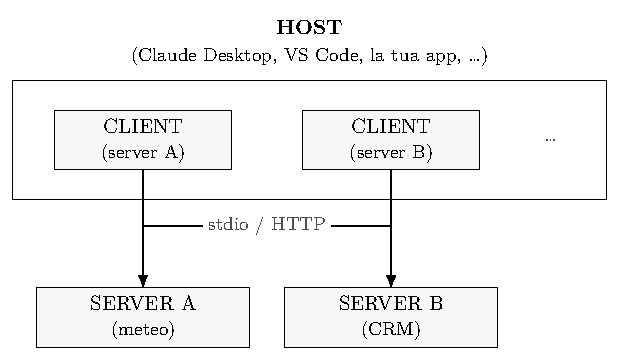
\includegraphics[keepaspectratio,alt={Architettura di
MCP: un host, uno o più client (uno per server) e i server che espongono
le capacità}]{figure/architettura.pdf}}
\caption{Architettura di MCP: un host, uno o più client (uno per server)
e i server che espongono le capacità}
\end{figure}

Ogni client è legato a \textbf{un solo server}: la specifica prevede una
relazione 1:1 tra client e server all'interno della sessione. L'host,
invece, aggrega più client e orchestra il modello, passandogli i
risultati dei vari server sotto forma di messaggi.

\subsection{1.3.1 Cosa fa l'host}\label{cosa-fa-lhost}

L'host è il regista della conversazione:

\begin{enumerate}
\def\labelenumi{\arabic{enumi}.}
\tightlist
\item
  avvia i client e, tramite loro, i server (nel caso di \texttt{stdio}
  li lancia come processi figli);
\item
  raccoglie le capabilities dei server (quali tool, risorse e prompt
  offrono);
\item
  presenta questi strumenti al modello linguistico (tipicamente
  iniettandone le descrizioni nel prompt di sistema);
\item
  quando il modello decide di chiamare uno strumento, l'host inoltra la
  richiesta al client giusto;
\item
  restituisce al modello il risultato, permettendogli di continuare il
  ragionamento.
\end{enumerate}

Nota bene: \textbf{il server non parla mai direttamente con il modello}.
È l'host che media. Il server si limita a esporre funzioni e dati; è il
modello, tramite l'host, a decidere se e quando usarli.

\subsection{1.3.2 Cosa fa il client}\label{cosa-fa-il-client}

Il client è un componente ``meccanico'': gestisce la connessione,
serializza e deserializza i messaggi JSON-RPC, mantiene lo stato della
sessione (handshake, negoziazione delle capabilities) e inoltra le
risposte all'host. Negli SDK, il client è quasi sempre una classe già
pronta: per noi, nel ruolo di sviluppatori del server, il client è
soprattutto il ``chiamante'' che invierà i messaggi.

\subsection{1.3.3 Cosa fa il server}\label{cosa-fa-il-server}

Il server è il nostro oggetto di studio. Le sue responsabilità sono:

\begin{itemize}
\tightlist
\item
  dichiarare le proprie \textbf{capabilities} durante l'handshake
  iniziale;
\item
  rispondere alle richieste di \textbf{discovery} (elenco dei tool,
  delle risorse, dei prompt);
\item
  \textbf{eseguire} le operazioni richieste (invocare un tool, leggere
  una risorsa, comporre un prompt);
\item
  restituire risultati strutturati, eventualmente con contenuti testuali
  e immagini;
\item
  notificare al client eventuali \textbf{eventi} asincroni (per esempio
  il cambiamento di una risorsa).
\end{itemize}

Nel C\# SDK gran parte di questo lavoro è automatizzato: come vedremo,
per esporre un tool basterà marcare un metodo C\# con un attributo.
L'SDK si occupa di introspezione, serializzazione, discovery e gestione
del trasporto.

\subsection{1.3.4 La negoziazione delle
capabilities}\label{la-negoziazione-delle-capabilities}

MCP è un protocollo \emph{capace di evolvere}: non tutti i client e i
server supportano tutte le funzionalità. Per questo, durante
l'handshake, client e server si scambiano le rispettive
\textbf{capabilities}, cioè un elenco dichiarativo di ciò che sanno
fare.

Il client dichiara, tra le altre cose:

\begin{itemize}
\tightlist
\item
  se supporta il \textbf{sampling} (permettere al server di chiedere
  generazione al modello);
\item
  se supporta le \textbf{roots} (informare il server sulle cartelle o
  sugli ambiti di lavoro);
\item
  se supporta la gestione di \textbf{tool, risorse e prompt}.
\end{itemize}

Il server dichiara:

\begin{itemize}
\tightlist
\item
  se espone \textbf{tool} (e con quali funzionalità);
\item
  se espone \textbf{risorse} (e se supporta le sottoscrizioni ai
  cambiamenti);
\item
  se espone \textbf{prompt};
\item
  se supporta il \textbf{logging} (inviare messaggi di log al client);
\item
  eventuali estensioni sperimentali.
\end{itemize}

Il risultato è che un server molto semplice (solo tool) e un client
molto semplice (solo tool) possono comunque comunicare correttamente,
ignorando le funzionalità non condivise. Quando, più avanti, useremo
l'SDK .NET, vedremo che la negoziazione avviene in modo automatico: a
noi basterà dichiarare ciò che il server espone, e l'SDK costruirà la
risposta di inizializzazione corretta.

\section{1.4 I primitivi del protocollo: Tools, Resources e
Prompts}\label{i-primitivi-del-protocollo-tools-resources-e-prompts}

Il cuore di MCP è costituito da tre primitivi, a cui se ne aggiungono
alcuni secondari. Comprenderli a fondo è indispensabile, perché tutto il
codice che scriveremo ruota attorno a essi.

\subsection{1.4.1 Tools: le azioni}\label{tools-le-azioni}

Un \textbf{tool} è una funzione che il server mette a disposizione del
modello. Quando il modello ``chiama'' un tool, invia al server un nome e
una lista di argomenti; il server esegue la funzione e restituisce un
risultato.

Ogni tool è descritto da:

\begin{itemize}
\tightlist
\item
  un \textbf{nome} (stringa, univoco all'interno del server);
\item
  una \textbf{descrizione} testuale, che il modello usa per capire
  \emph{quando} e \emph{come} usarlo: una buona descrizione è il fattore
  che più influenza la qualità dell'uso;
\item
  uno \textbf{schema JSON} degli argomenti in ingresso (nome, tipo,
  obbligatorietà, descrizione di ogni parametro);
\item
  opzionalmente, uno schema dell'output.
\end{itemize}

Esempi tipici di tool: \texttt{search\_documents}, \texttt{send\_email},
\texttt{create\_ticket}, \texttt{get\_weather}, \texttt{read\_file},
\texttt{run\_query}. Un tool può essere \textbf{idempotente} o meno,
\textbf{che modifica lo stato} o di sola lettura: MCP prevede
annotazioni facoltative per dichiararlo (ci torneremo).

È importante capire la direzione del flusso: nei tool è il
\textbf{modello} a prendere l'iniziativa. Il server espone il menu, il
modello sceglie dal menu e il server esegue.

\subsection{1.4.2 Resources: i dati}\label{resources-i-dati}

Una \textbf{resource} è un dato esposto dal server e identificato da un
\textbf{URI}. Se i tool sono le ``azioni'', le risorse sono i
``documenti'': file, record, configurazioni, immagini, log. Il modello
(o il client, per conto dell'utente) può \emph{leggere} una risorsa per
acquisire contesto.

Le risorse hanno una differenza concettuale fondamentale rispetto ai
tool: nei tool il controllo è del modello, nelle risorse il controllo è
\textbf{del client o dell'applicazione}. Un'applicazione può decidere
autonomamente di ``agganciare'' una risorsa al contesto del modello,
senza che il modello debba chiederla.

Le risorse possono essere:

\begin{itemize}
\tightlist
\item
  \textbf{statiche}, con un URI fisso (per esempio
  \texttt{config://app/settings});
\item
  \textbf{parametrizzate tramite template}, in cui l'URI contiene dei
  segnaposto (per esempio \texttt{file://docs/\{id\}}): il client può
  elencare i template e poi leggere una risorsa concreta sostituendo i
  parametri.
\end{itemize}

Ogni risorsa dichiara un \textbf{tipo MIME} (per esempio
\texttt{text/plain}, \texttt{application/json}, \texttt{image/png}),
così il client sa come interpretarla.

\subsection{1.4.3 Prompts: i modelli di
istruzione}\label{prompts-i-modelli-di-istruzione}

Un \textbf{prompt} è un modello di istruzioni riutilizzabile, esposto
dal server e richiamabile dal client o dall'utente. Mentre un tool
\emph{esegue} qualcosa, un prompt \emph{produce testo} (o una sequenza
di messaggi) pronto per essere inviato al modello.

Un caso d'uso tipico: il server espone un prompt \texttt{review\_code}
che, dato un frammento di codice, produce il testo ``Fai una revisione
approfondita del seguente codice, segnalando bug, problemi di sicurezza
e suggerimenti di stile: \ldots{}''. L'utente, dall'interfaccia
dell'host, può selezionare il prompt senza doverlo riscrivere.

I prompt possono dichiarare \textbf{argomenti} (con schema JSON), e la
loro esecuzione restituisce una lista di messaggi (ruolo + contenuto),
non necessariamente una singola stringa.

\subsection{1.4.4 Gli altri primitivi}\label{gli-altri-primitivi}

Oltre ai tre principali, la specifica prevede primitivi più avanzati,
che non implementeremo in dettaglio ma che è bene conoscere:

\begin{itemize}
\tightlist
\item
  \textbf{Sampling} --- permette al \emph{server} di chiedere al
  \emph{client} di generare testo con il modello. Utile per scenari in
  cui il server deve, per esempio, riassumere un documento.
\item
  \textbf{Roots} --- permette al client di comunicare al server quali
  sono le ``radici'' del progetto (cartelle, URL) su cui l'utente sta
  lavorando.
\item
  \textbf{Elicitation} --- permette al server di porre una domanda
  all'utente durante l'esecuzione di un tool.
\item
  \textbf{Logging} --- permette al server di inviare messaggi di log
  strutturati al client.
\item
  \textbf{Completions} --- permette al server di suggerire completamenti
  per gli argomenti dei prompt.
\item
  \textbf{Pagination e Progress} --- per gestire elenchi lunghi e
  operazioni lente.
\end{itemize}

\subsection{1.4.5 La tabella riassuntiva}\label{la-tabella-riassuntiva}

{\def\LTcaptype{none} % do not increment counter
\begin{longtable}[]{@{}lll@{}}
\toprule\noalign{}
Primitivo & Chi lo attiva & A cosa serve \\
\midrule\noalign{}
\endhead
\bottomrule\noalign{}
\endlastfoot
Tool & Modello & Eseguire azioni \\
Resource & Client / app & Fornire contesto \\
Prompt & Utente / client & Preparare istruzioni \\
\end{longtable}
}

Tenere a mente questa tabella aiuta a scegliere il primitivo giusto
quando si progetta un server: se il modello deve \emph{fare} qualcosa,
serve un tool; se deve \emph{leggere} qualcosa, una resource; se
l'utente deve \emph{invocare un'istruzione pronta}, un prompt.

\section{1.5 JSON-RPC 2.0: il linguaggio del
protocollo}\label{json-rpc-2.0-il-linguaggio-del-protocollo}

Tutta la comunicazione MCP avviene tramite messaggi \textbf{JSON-RPC
2.0}. JSON-RPC è un protocollo remoto estremamente semplice: un
messaggio JSON che descrive una chiamata di procedura remota, con un
identificatore per correlare richieste e risposte. Se hai mai lavorato
con RPC, gRPC o con le API JSON di Ethereum, il concetto ti sarà
familiare.

MCP usa JSON-RPC 2.0 con alcune convenzioni specifiche. I tipi di
messaggio sono tre: request, notification e response; l'errore è una
variante della response.

\subsection{1.5.1 La richiesta (request)}\label{la-richiesta-request}

Una richiesta è un messaggio inviato da una parte per chiedere all'altra
di eseguire un'operazione. Ha un campo \texttt{method} e, opzionalmente,
un campo \texttt{params}:

\begin{Shaded}
\begin{Highlighting}[]
\FunctionTok{\{}
  \DataTypeTok{"jsonrpc"}\FunctionTok{:} \StringTok{"2.0"}\FunctionTok{,}
  \DataTypeTok{"id"}\FunctionTok{:} \DecValTok{1}\FunctionTok{,}
  \DataTypeTok{"method"}\FunctionTok{:} \StringTok{"tools/call"}\FunctionTok{,}
  \DataTypeTok{"params"}\FunctionTok{:} \FunctionTok{\{}
    \DataTypeTok{"name"}\FunctionTok{:} \StringTok{"echo"}\FunctionTok{,}
    \DataTypeTok{"arguments"}\FunctionTok{:} \FunctionTok{\{} \DataTypeTok{"message"}\FunctionTok{:} \StringTok{"ciao"} \FunctionTok{\}}
  \FunctionTok{\}}
\FunctionTok{\}}
\end{Highlighting}
\end{Shaded}

Il campo \texttt{id} può essere una stringa o un numero e serve a
correlare la risposta. Quando l'operazione non richiede risposta, il
messaggio diventa una \emph{notifica} (vedi sotto) e l'\texttt{id} viene
omesso.

\subsection{1.5.2 La risposta (response)}\label{la-risposta-response}

La risposta a una richiesta riporta lo stesso \texttt{id} e il risultato
nel campo \texttt{result}:

\begin{Shaded}
\begin{Highlighting}[]
\FunctionTok{\{}
  \DataTypeTok{"jsonrpc"}\FunctionTok{:} \StringTok{"2.0"}\FunctionTok{,}
  \DataTypeTok{"id"}\FunctionTok{:} \DecValTok{1}\FunctionTok{,}
  \DataTypeTok{"result"}\FunctionTok{:} \FunctionTok{\{}
    \DataTypeTok{"content"}\FunctionTok{:} \OtherTok{[}
      \FunctionTok{\{} \DataTypeTok{"type"}\FunctionTok{:} \StringTok{"text"}\FunctionTok{,} \DataTypeTok{"text"}\FunctionTok{:} \StringTok{"hello ciao"} \FunctionTok{\}}
    \OtherTok{]}\FunctionTok{,}
    \DataTypeTok{"isError"}\FunctionTok{:} \KeywordTok{false}
  \FunctionTok{\}}
\FunctionTok{\}}
\end{Highlighting}
\end{Shaded}

\subsection{1.5.3 La variante di errore della
risposta}\label{la-variante-di-errore-della-risposta}

In caso di errore a livello di protocollo, la risposta contiene un campo
\texttt{error} al posto di \texttt{result}. Non è un quarto tipo di
messaggio, ma una variante della response:

\begin{Shaded}
\begin{Highlighting}[]
\FunctionTok{\{}
  \DataTypeTok{"jsonrpc"}\FunctionTok{:} \StringTok{"2.0"}\FunctionTok{,}
  \DataTypeTok{"id"}\FunctionTok{:} \DecValTok{1}\FunctionTok{,}
  \DataTypeTok{"error"}\FunctionTok{:} \FunctionTok{\{}
    \DataTypeTok{"code"}\FunctionTok{:} \DecValTok{{-}32602}\FunctionTok{,}
    \DataTypeTok{"message"}\FunctionTok{:} \StringTok{"Invalid params"}
  \FunctionTok{\}}
\FunctionTok{\}}
\end{Highlighting}
\end{Shaded}

I codici di errore standard di JSON-RPC, che MCP riusa, sono:

{\def\LTcaptype{none} % do not increment counter
\begin{longtable}[]{@{}ll@{}}
\toprule\noalign{}
Codice & Significato \\
\midrule\noalign{}
\endhead
\bottomrule\noalign{}
\endlastfoot
-32700 & Parse error \\
-32600 & Invalid request \\
-32601 & Method not found \\
-32602 & Invalid params \\
-32603 & Internal error \\
\end{longtable}
}

A questi MCP aggiunge codici specifici, come \texttt{-32002} (resource
not found) o \texttt{-32022} (unsupported protocol version). Nell'SDK
.NET questi valori sono raccolti nell'enumerazione
\texttt{McpErrorCode}, che useremo nella sezione sulla gestione degli
errori.

Un errore durante l'esecuzione di un tool è diverso: \texttt{tools/call}
restituisce comunque un \texttt{result}, il cui \texttt{CallToolResult}
segnala \texttt{isError:\ true}.

\subsection{1.5.4 La notifica
(notification)}\label{la-notifica-notification}

Una notifica è una richiesta \emph{senza} \texttt{id}: il destinatario
la esegue ma non deve rispondere. Si usa per eventi unidirezionali.
L'esempio più importante è la notifica di inizializzazione completata:

\begin{Shaded}
\begin{Highlighting}[]
\FunctionTok{\{}
  \DataTypeTok{"jsonrpc"}\FunctionTok{:} \StringTok{"2.0"}\FunctionTok{,}
  \DataTypeTok{"method"}\FunctionTok{:} \StringTok{"notifications/initialized"}\FunctionTok{,}
  \DataTypeTok{"params"}\FunctionTok{:} \FunctionTok{\{\}}
\FunctionTok{\}}
\end{Highlighting}
\end{Shaded}

\subsection{1.5.5 I metodi standard di
MCP}\label{i-metodi-standard-di-mcp}

Sopra JSON-RPC, MCP definisce una serie di metodi con nomi a barre
(\texttt{risorsa/azione}). I più importanti, lato server:

{\def\LTcaptype{none} % do not increment counter
\begin{longtable}[]{@{}
  >{\raggedright\arraybackslash}p{(\linewidth - 2\tabcolsep) * \real{0.5333}}
  >{\raggedright\arraybackslash}p{(\linewidth - 2\tabcolsep) * \real{0.4667}}@{}}
\toprule\noalign{}
\begin{minipage}[b]{\linewidth}\raggedright
Metodo
\end{minipage} & \begin{minipage}[b]{\linewidth}\raggedright
Scopo
\end{minipage} \\
\midrule\noalign{}
\endhead
\bottomrule\noalign{}
\endlastfoot
\texttt{initialize} & Avvia la sessione e negozia le capabilities \\
\texttt{notifications/initialized} & Notifica che l'inizializzazione è
conclusa \\
\texttt{ping} & Verifica che la connessione sia viva \\
\texttt{tools/list} & Elenca i tool disponibili \\
\texttt{tools/call} & Invoca un tool \\
\texttt{resources/list} & Elenca le risorse \\
\texttt{resources/read} & Legge una risorsa \\
\texttt{resources/templates/list} & Elenca i template di risorsa \\
\texttt{prompts/list} & Elenca i prompt \\
\texttt{prompts/get} & Ottiene un prompt \\
\texttt{logging/setLevel} & Imposta il livello di log \\
\texttt{completion/complete} & Richiede completamenti \\
\end{longtable}
}

Il bello di lavorare con l'SDK .NET è che \textbf{non dovremo mai
scrivere questi messaggi a mano}: l'SDK li genera e li interpreta per
noi. Conoscerli, però, è essenziale per il debugging, per leggere i log
e per capire cosa succede ``sotto il cofano''. Inoltre, quando useremo
l'MCP Inspector o un client generico, sarà naturale ragionare in termini
di questi metodi.

\subsection{1.5.6 Un esempio completo di
scambio}\label{un-esempio-completo-di-scambio}

Mettiamo insieme i pezzi per vedere una sessione minima. Il client apre
la connessione e invia l'inizializzazione:

\begin{Shaded}
\begin{Highlighting}[]
\FunctionTok{\{}\DataTypeTok{"jsonrpc"}\FunctionTok{:}\StringTok{"2.0"}\FunctionTok{,}\DataTypeTok{"id"}\FunctionTok{:}\DecValTok{1}\FunctionTok{,}\DataTypeTok{"method"}\FunctionTok{:}\StringTok{"initialize"}\FunctionTok{,}\DataTypeTok{"params"}\FunctionTok{:\{}
  \DataTypeTok{"protocolVersion"}\FunctionTok{:}\StringTok{"2025{-}06{-}18"}\FunctionTok{,}
  \DataTypeTok{"capabilities"}\FunctionTok{:\{\},}
  \DataTypeTok{"clientInfo"}\FunctionTok{:\{}\DataTypeTok{"name"}\FunctionTok{:}\StringTok{"book{-}test"}\FunctionTok{,}\DataTypeTok{"version"}\FunctionTok{:}\StringTok{"1.0"}\FunctionTok{\}}
\FunctionTok{\}\}}
\end{Highlighting}
\end{Shaded}

Il server risponde con le proprie informazioni e capacità:

\begin{Shaded}
\begin{Highlighting}[]
\FunctionTok{\{}\DataTypeTok{"jsonrpc"}\FunctionTok{:}\StringTok{"2.0"}\FunctionTok{,}\DataTypeTok{"id"}\FunctionTok{:}\DecValTok{1}\FunctionTok{,}\DataTypeTok{"result"}\FunctionTok{:\{}
  \DataTypeTok{"protocolVersion"}\FunctionTok{:}\StringTok{"2025{-}06{-}18"}\FunctionTok{,}
  \DataTypeTok{"capabilities"}\FunctionTok{:\{}\DataTypeTok{"tools"}\FunctionTok{:\{\}\},}
  \DataTypeTok{"serverInfo"}\FunctionTok{:\{}\DataTypeTok{"name"}\FunctionTok{:}\StringTok{"McpTest"}\FunctionTok{,}\DataTypeTok{"version"}\FunctionTok{:}\StringTok{"1.0.0.0"}\FunctionTok{\}}
\FunctionTok{\}\}}
\end{Highlighting}
\end{Shaded}

Il client notifica che l'inizializzazione è completa e poi elenca i
tool:

\begin{Shaded}
\begin{Highlighting}[]
\FunctionTok{\{}\DataTypeTok{"jsonrpc"}\FunctionTok{:}\StringTok{"2.0"}\FunctionTok{,}\DataTypeTok{"method"}\FunctionTok{:}\StringTok{"notifications/initialized"}\FunctionTok{,}\DataTypeTok{"params"}\FunctionTok{:\{\}\}}
\FunctionTok{\{}\DataTypeTok{"jsonrpc"}\FunctionTok{:}\StringTok{"2.0"}\FunctionTok{,}\DataTypeTok{"id"}\FunctionTok{:}\DecValTok{2}\FunctionTok{,}\DataTypeTok{"method"}\FunctionTok{:}\StringTok{"tools/list"}\FunctionTok{,}\DataTypeTok{"params"}\FunctionTok{:\{\}\}}
\end{Highlighting}
\end{Shaded}

Il server risponde con l'elenco (nota il nome in minuscolo, un dettaglio
dell'SDK che documenteremo):

\begin{Shaded}
\begin{Highlighting}[]
\FunctionTok{\{}\DataTypeTok{"jsonrpc"}\FunctionTok{:}\StringTok{"2.0"}\FunctionTok{,}\DataTypeTok{"id"}\FunctionTok{:}\DecValTok{2}\FunctionTok{,}\DataTypeTok{"result"}\FunctionTok{:\{}\DataTypeTok{"tools"}\FunctionTok{:}\OtherTok{[}
  \FunctionTok{\{}\DataTypeTok{"name"}\FunctionTok{:}\StringTok{"echo"}\FunctionTok{,}\DataTypeTok{"description"}\FunctionTok{:}\StringTok{"Echoes the message back to the client."}\FunctionTok{,}
   \DataTypeTok{"inputSchema"}\FunctionTok{:\{}\DataTypeTok{"type"}\FunctionTok{:}\StringTok{"object"}\FunctionTok{,}\DataTypeTok{"properties"}\FunctionTok{:\{}
      \DataTypeTok{"message"}\FunctionTok{:\{}\DataTypeTok{"type"}\FunctionTok{:}\StringTok{"string"}\FunctionTok{,}\DataTypeTok{"description"}\FunctionTok{:}\StringTok{"The message to echo."}\FunctionTok{\}\},}
    \DataTypeTok{"required"}\FunctionTok{:}\OtherTok{[}\StringTok{"message"}\OtherTok{]}\FunctionTok{\}\}}
\OtherTok{]}\FunctionTok{\}\}}
\end{Highlighting}
\end{Shaded}

Infine il client invoca il tool:

\begin{Shaded}
\begin{Highlighting}[]
\FunctionTok{\{}\DataTypeTok{"jsonrpc"}\FunctionTok{:}\StringTok{"2.0"}\FunctionTok{,}\DataTypeTok{"id"}\FunctionTok{:}\DecValTok{3}\FunctionTok{,}\DataTypeTok{"method"}\FunctionTok{:}\StringTok{"tools/call"}\FunctionTok{,}\DataTypeTok{"params"}\FunctionTok{:\{}
  \DataTypeTok{"name"}\FunctionTok{:}\StringTok{"echo"}\FunctionTok{,}\DataTypeTok{"arguments"}\FunctionTok{:\{}\DataTypeTok{"message"}\FunctionTok{:}\StringTok{"mondo"}\FunctionTok{\}\}\}}
\end{Highlighting}
\end{Shaded}

E il server restituisce il risultato:

\begin{Shaded}
\begin{Highlighting}[]
\FunctionTok{\{}\DataTypeTok{"jsonrpc"}\FunctionTok{:}\StringTok{"2.0"}\FunctionTok{,}\DataTypeTok{"id"}\FunctionTok{:}\DecValTok{3}\FunctionTok{,}\DataTypeTok{"result"}\FunctionTok{:\{}
  \DataTypeTok{"content"}\FunctionTok{:}\OtherTok{[}\FunctionTok{\{}\DataTypeTok{"type"}\FunctionTok{:}\StringTok{"text"}\FunctionTok{,}\DataTypeTok{"text"}\FunctionTok{:}\StringTok{"hello mondo"}\FunctionTok{\}}\OtherTok{]}\FunctionTok{,}
  \DataTypeTok{"isError"}\FunctionTok{:}\KeywordTok{false}
\FunctionTok{\}\}}
\end{Highlighting}
\end{Shaded}

Questo scambio, pur minimale, contiene tutto il DNA di MCP. Lo rivedremo
realizzato davvero, byte per byte, quando eseguiremo il nostro primo
server.

\section{1.6 I trasporti: stdio, Streamable HTTP e
SSE}\label{i-trasporti-stdio-streamable-http-e-sse}

JSON-RPC definisce \emph{cosa} si dice, ma non \emph{come} lo si
trasporta. MCP definisce una famiglia di \textbf{trasporti}: canali
concreti su cui i messaggi viaggiano. La scelta del trasporto è una
delle decisioni progettuali più importanti, perché determina dove e come
il server verrà eseguito.

\subsection{1.6.1 stdio: il trasporto dei processi
locali}\label{stdio-il-trasporto-dei-processi-locali}

Nel trasporto \texttt{stdio}, il server viene \textbf{lanciato come
processo figlio} dal client, e la comunicazione avviene attraverso lo
standard input e lo standard output del processo:

\begin{itemize}
\tightlist
\item
  il client scrive i messaggi JSON-RPC sullo \textbf{stdin} del server;
\item
  il server risponde sullo \textbf{stdout};
\item
  i messaggi sono delimitati da \textbf{newline} (un oggetto JSON per
  riga).
\end{itemize}

È il trasporto più semplice e più diffuso per i server locali: non
richiede porte di rete, né configurazioni di firewall, né esposizione a
Internet. Il ciclo di vita del server coincide con quello del processo:
quando il client si chiude (o lo stdin raggiunge la fine), il server
termina.

La conseguenza pratica più importante, che vale la pena evidenziare
subito, è questa: \textbf{su \texttt{stdio} lo stdout appartiene al
protocollo}. Qualsiasi altra scrittura sullo stdout --- per esempio i
log della console --- corrompe il flusso JSON-RPC e rende il server
inutilizzabile. Per questo, nei nostri server \texttt{stdio},
disabiliteremo il logging su console con
\texttt{builder.Logging.ClearProviders()}.

\subsection{1.6.2 Streamable HTTP: il trasporto di
rete}\label{streamable-http-il-trasporto-di-rete}

Il trasporto \textbf{Streamable HTTP} è il trasporto di rete
raccomandato dalla specifica moderna. Il server espone un
\textbf{singolo endpoint HTTP} (per esempio
\texttt{http://localhost:8080/mcp}) e:

\begin{itemize}
\tightlist
\item
  il client invia le richieste JSON-RPC con normali richieste
  \texttt{POST};
\item
  il server può rispondere direttamente nel body della risposta (per le
  richieste singole) oppure aprire uno \textbf{stream} (per esempio con
  Server-Sent Events) per inviare risposte e notifiche multiple nel
  tempo.
\end{itemize}

Streamable HTTP è pensato per funzionare bene con i load balancer, i
reverse proxy e i meccanismi standard di HTTP (autenticazione, TLS,
cache). Supporta anche una modalità \textbf{stateless}, in cui ogni
richiesta è indipendente e il server non mantiene una sessione
persistente.

\subsection{1.6.3 Il vecchio trasporto
HTTP+SSE}\label{il-vecchio-trasporto-httpsse}

La prima versione di MCP definiva un trasporto HTTP basato su due
endpoint: uno per le richieste del client e uno per lo stream di eventi
del server (SSE). Questo trasporto è oggi \textbf{deprecato} in favore
di Streamable HTTP, ma lo si incontra ancora in molti server esistenti e
in molta documentazione. L'SDK .NET lo supporta ancora (con l'opzione
\texttt{EnableLegacySse}), per compatibilità.

\subsection{1.6.4 Come scegliere il
trasporto}\label{come-scegliere-il-trasporto}

{\def\LTcaptype{none} % do not increment counter
\begin{longtable}[]{@{}
  >{\raggedright\arraybackslash}p{(\linewidth - 2\tabcolsep) * \real{0.2941}}
  >{\raggedright\arraybackslash}p{(\linewidth - 2\tabcolsep) * \real{0.7059}}@{}}
\toprule\noalign{}
\begin{minipage}[b]{\linewidth}\raggedright
Scenario
\end{minipage} & \begin{minipage}[b]{\linewidth}\raggedright
Trasporto consigliato
\end{minipage} \\
\midrule\noalign{}
\endhead
\bottomrule\noalign{}
\endlastfoot
Server personale, usato da un client locale sulla stessa macchina &
\texttt{stdio} \\
Server condiviso tra più utenti o macchine & Streamable HTTP \\
Server in un container o dietro un proxy/reverse proxy & Streamable
HTTP \\
Server che deve inviare eventi asincroni frequenti & Streamable HTTP \\
Integrazione con un IDE (VS Code, ecc.) & \texttt{stdio} o HTTP, a
seconda del caso \\
\end{longtable}
}

In questo capitolo implementeremo entrambi: prima un server
\texttt{stdio} completo, poi la sua versione HTTP con ASP.NET Core, in
modo da padroneggiare l'intero spettro.

\subsection{1.6.5 Il ruolo dell'SDK}\label{il-ruolo-dellsdk}

Da sviluppatori non dobbiamo occuparci dei dettagli di framing: l'SDK
.NET fornisce i trasporti già pronti. In particolare, nel pacchetto
troviamo le classi \texttt{StdioServerTransport},
\texttt{StreamableHttpServerTransport} e \texttt{StreamServerTransport},
che vengono selezionate con un semplice metodo di configurazione
(\texttt{WithStdioServerTransport()}, \texttt{WithHttpTransport()}). La
nostra responsabilità si riduce a scegliere il trasporto giusto e a
rispettare le sue regole (per esempio, non scrivere sullo stdout nei
server \texttt{stdio}).

\section{1.7 Il ciclo di vita di una sessione
MCP}\label{il-ciclo-di-vita-di-una-sessione-mcp}

Una sessione MCP attraversa fasi ben precise, regolate dalla specifica.
Conoscerle aiuta a capire gli errori di connessione e a progettare
server robusti.

\subsection{1.7.1 Fase 1:
l'inizializzazione}\label{fase-1-linizializzazione}

Appena la connessione è stabilita, il client invia una richiesta
\texttt{initialize} con:

\begin{itemize}
\tightlist
\item
  la \textbf{versione del protocollo} che intende usare;
\item
  le proprie \textbf{capabilities};
\item
  le proprie informazioni (\texttt{clientInfo}: nome e versione).
\end{itemize}

Il server risponde dichiarando:

\begin{itemize}
\tightlist
\item
  la versione del protocollo \textbf{effettiva} (che deve essere
  compatibile con quella richiesta);
\item
  le proprie \textbf{capabilities};
\item
  le proprie informazioni (\texttt{serverInfo});
\item
  facoltativamente, le \textbf{istruzioni} per il modello (un testo che
  l'host può includere nel prompt di sistema per spiegare come usare il
  server).
\end{itemize}

Le versioni del protocollo sono identificate da una data (per esempio
\texttt{2025-06-18}), non seguono il versionamento semantico dei
pacchetti. Client e server negoziano una versione supportata; se non è
possibile concordarne una, la sessione non può essere inizializzata.

\subsection{1.7.2 Fase 2: la notifica di
``initialized''}\label{fase-2-la-notifica-di-initialized}

Dopo aver ricevuto la risposta a \texttt{initialize}, il client invia la
\textbf{notifica} \texttt{notifications/initialized}. Solo da questo
momento in poi il client è autorizzato a inviare richieste ``normali''
(elencare i tool, invocarli, ecc.). Un server corretto deve quindi
\textbf{rifiutare le richieste che arrivano prima
dell'inizializzazione}. L'SDK .NET applica questa regola
automaticamente.

\subsection{1.7.3 Fase 3: l'operatività}\label{fase-3-loperativituxe0}

In questa fase avviene il lavoro vero e proprio: discovery, invocazione
di tool, lettura di risorse, recupero di prompt. Le due parti possono
inoltre scambiarsi:

\begin{itemize}
\tightlist
\item
  \texttt{ping} per verificare che la connessione sia viva;
\item
  notifiche di log e di cambiamento delle risorse;
\item
  richieste di sampling (dal server verso il client).
\end{itemize}

\subsection{1.7.4 Fase 4: la chiusura}\label{fase-4-la-chiusura}

La sessione termina quando:

\begin{itemize}
\tightlist
\item
  una delle parti chiude il trasporto (per \texttt{stdio}, quando il
  processo termina o lo stdin si chiude);
\item
  il client invia una richiesta di chiusura esplicita (se il trasporto
  la prevede);
\item
  scatta un timeout o un errore irreversibile.
\end{itemize}

Non esiste un metodo \texttt{shutdown} universale nella specifica base:
la chiusura è, di norma, legata alla vita del trasporto. Per un server
\texttt{stdio} questo significa che il processo deve uscire in modo
pulito quando lo stdin viene chiuso; l'SDK gestisce anche questo per
noi.

\subsection{1.7.5 La sequenza riassunta}\label{la-sequenza-riassunta}

\begin{figure}
\centering
\pandocbounded{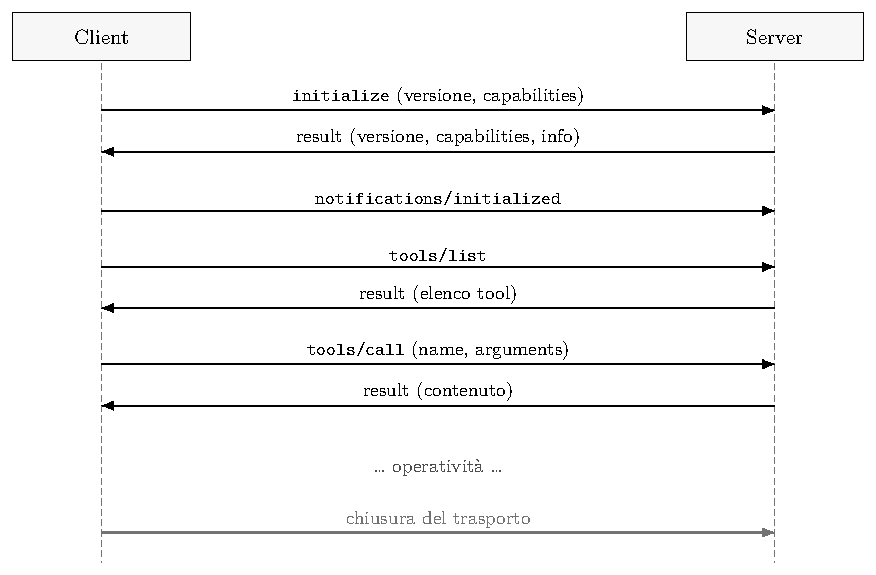
\includegraphics[keepaspectratio,alt={Sequenza completa
del ciclo di vita di una sessione MCP}]{figure/lifecycle.pdf}}
\caption{Sequenza completa del ciclo di vita di una sessione MCP}
\end{figure}

\subsection{1.7.6 Cosa significa per il nostro
codice}\label{cosa-significa-per-il-nostro-codice}

Tutta questa sequenza è gestita dall'SDK. La nostra unica accortezza,
nel caso del trasporto \texttt{stdio}, sarà ricordare che il processo
deve restare in esecuzione in attesa di messaggi, e che lo stdout è
riservato al protocollo. Nelle prossime sezioni vedremo come il template
\texttt{Host.CreateApplicationBuilder} + \texttt{RunAsync()} realizzi
esattamente questo ciclo di vita in poche righe.

\section{1.8 MCP vs REST API: un confronto
approfondito}\label{mcp-vs-rest-api-un-confronto-approfondito}

``Ma io ho già le mie API REST: perché dovrei usare MCP?'' È la domanda
più frequente, e la risposta merita una sezione intera. La chiave è
capire che \textbf{non sono concorrenti}: risolvono problemi diversi e,
nella maggior parte dei progetti reali, convivono.

\subsection{1.8.1 Cos'è una REST API}\label{cosuxe8-una-rest-api}

Una REST API (Representational State Transfer) è uno stile
architettonico per esporre risorse su HTTP. Un servizio definisce una
serie di \textbf{endpoint} (URL) e di \textbf{verbi HTTP} (GET, POST,
PUT, DELETE), con formati di richiesta e risposta (tipicamente JSON)
documentati a mano o con specifiche come OpenAPI.

Esempio:

\begin{Shaded}
\begin{Highlighting}[]
\NormalTok{GET    /api/customers/123}
\NormalTok{POST   /api/customers}
\NormalTok{PUT    /api/customers/123}
\NormalTok{DELETE /api/customers/123}
\end{Highlighting}
\end{Shaded}

Le REST API sono ottime per la comunicazione \textbf{tra software}:
un'applicazione chiama un'altra applicazione in modo deterministico,
tipizzato e prevedibile. Il chiamante sa \emph{esattamente} quale
endpoint invocare e quali parametri passare.

\subsection{1.8.2 Cos'è un MCP server}\label{cosuxe8-un-mcp-server}

Un MCP server, come abbiamo visto, espone \textbf{tool, risorse e
prompt} descritti in modo autodescrittivo e \emph{scopribili}. Il
chiamante non conosce a priori gli endpoint: all'avvio chiede al server
``che cosa sai fare?'' e riceve un elenco di funzionalità con relative
descrizioni e schemi. La decisione su \emph{cosa} invocare spetta al
\textbf{modello}, non a un programmatore che ha scritto il codice di
integrazione.

\subsection{1.8.3 La differenza fondamentale: chi decide cosa
chiamare}\label{la-differenza-fondamentale-chi-decide-cosa-chiamare}

\small

{\def\LTcaptype{none} % do not increment counter
\begin{longtable}[]{@{}
  >{\raggedright\arraybackslash}p{(\linewidth - 4\tabcolsep) * \real{0.2414}}
  >{\raggedright\arraybackslash}p{(\linewidth - 4\tabcolsep) * \real{0.3448}}
  >{\raggedright\arraybackslash}p{(\linewidth - 4\tabcolsep) * \real{0.4138}}@{}}
\toprule\noalign{}
\begin{minipage}[b]{\linewidth}\raggedright
\end{minipage} & \begin{minipage}[b]{\linewidth}\raggedright
REST API
\end{minipage} & \begin{minipage}[b]{\linewidth}\raggedright
MCP server
\end{minipage} \\
\midrule\noalign{}
\endhead
\bottomrule\noalign{}
\endlastfoot
\textbf{Consumatore} & Un'applicazione (codice scritto da un umano) & Un
modello linguistico (o un client che lo assiste) \\
\textbf{Scoperta} & Documentazione, OpenAPI, a mano & Automatica
(\texttt{tools/list}, \texttt{resources/list}, \ldots) \\
\textbf{Decisione di chiamata} & Il programmatore, a compile time & Il
modello, a runtime, in base al contesto \\
\textbf{Contratto} & Endpoint + verbi + schemi specifici per servizio &
Un unico protocollo per tutti i servizi \\
\textbf{Semantica} & Legata al dominio (\texttt{/customers},
\texttt{/orders}) & Generica (tool, risorse, prompt) \\
\textbf{Stato} & Stateless (di norma) & Sessione con capabilities
negoziate \\
\textbf{Trasporto tipico} & HTTP & \texttt{stdio}, Streamable HTTP \\
\end{longtable}
}

\normalsize

In una REST API il \textbf{programmatore} decide: scrive
\texttt{GET\ /api/weather?city=Roma} e conosce la risposta. In un MCP
server il \textbf{modello} decide: gli vengono presentati i tool
disponibili (``c'è un tool \texttt{get\_weather} che accetta
\texttt{city}'') e, quando l'utente chiede ``che tempo fa a Roma?'', il
modello capisce da solo di dover chiamare \texttt{get\_weather} con
\texttt{city\ =\ "Roma"}.

\subsection{1.8.4 L'autodescrizione è il vero
valore}\label{lautodescrizione-uxe8-il-vero-valore}

La differenza pratica più profonda è l'\textbf{autodescrizione}. Un MCP
server non espone solo funzioni: espone \emph{descrizioni} di quelle
funzioni, pensate per essere lette da un modello. Il nome, la
descrizione del tool e la descrizione di ogni parametro diventano parte
del ``prompt di sistema'' che l'host costruisce per il modello. La
qualità di queste descrizioni determina la probabilità che il modello
usi lo strumento correttamente.

Una REST API, per contro, è descritta da una documentazione pensata per
\textbf{umani} (o, nel migliore dei casi, da una specifica OpenAPI
pensata per generatori di codice). Un LLM può, in teoria, imparare a
usare un'API REST leggendone la documentazione, ma questo processo è
fragile e va ripetuto per ogni API.

\subsection{1.8.5 Il problema M×N, di
nuovo}\label{il-problema-mn-di-nuovo}

Torniamo al problema M×N. Con le REST API, ogni applicazione AI deve
essere integrata a mano con ogni servizio. Con MCP, ogni servizio espone
una volta la propria interfaccia standard, e \emph{tutte} le
applicazioni AI che parlano MCP possono usarla senza ulteriore lavoro. È
il passaggio da una complessità moltiplicativa a una complessità
additiva: \emph{M} applicazioni + \emph{N} server, invece di \emph{M ×
N} integrazioni.

\subsection{1.8.6 Quando usare cosa}\label{quando-usare-cosa}

\textbf{Usa una REST API quando:}

\begin{itemize}
\tightlist
\item
  il consumatore è un'applicazione o un servizio, non un LLM;
\item
  hai bisogno di controllo tipizzato, prestazioni prevedibili e
  semantica di dominio esplicita;
\item
  la logica di business richiede transazioni, versioning degli endpoint,
  contratti stabili;
\item
  devi esporre funzionalità a terze parti con un contratto pubblico ben
  definito.
\end{itemize}

\textbf{Usa un MCP server quando:}

\begin{itemize}
\tightlist
\item
  il consumatore è un'applicazione basata su LLM (assistenti, agenti,
  copiloti);
\item
  vuoi che il modello scopra e usi i tuoi strumenti e dati senza
  integrazioni ad hoc;
\item
  vuoi scrivere l'integrazione \textbf{una volta} e riusarla con
  qualsiasi host (Claude, VS Code, Copilot, un tuo agente);
\item
  vuoi esporre non solo dati, ma anche azioni e template di prompt in
  modo uniforme.
\end{itemize}

\textbf{La combinazione vincente} è, molto spesso, \textbf{entrambi}:
mantieni le tue REST API come strato applicativo, e costruisci un MCP
server che vi si appoggia sopra per renderle consumabili dai modelli. È
esattamente ciò che faremo nell'esempio meteo: il nostro MCP server
chiamerà un'API HTTP esterna e ne esporrà il risultato come tool.

\subsection{1.8.7 Un esempio concreto di
differenza}\label{un-esempio-concreto-di-differenza}

Consideriamo il caso ``cerca un volo''. Con una REST API:

\begin{Shaded}
\begin{Highlighting}[]
\NormalTok{GET /api/flights/search?from=FCO\&to=JFK\&date=2026{-}11{-}01}
\NormalTok{Authorization: Bearer \textless{}token\textgreater{}}
\end{Highlighting}
\end{Shaded}

Il chiamante deve conoscere l'endpoint, i parametri, l'autenticazione e
il formato della risposta. Con un MCP server, il client vede invece:

\begin{Shaded}
\begin{Highlighting}[]
\FunctionTok{\{}
  \DataTypeTok{"name"}\FunctionTok{:} \StringTok{"search\_flights"}\FunctionTok{,}
  \DataTypeTok{"description"}\FunctionTok{:} \StringTok{"Search available flights between two airports on a given date."}\FunctionTok{,}
  \DataTypeTok{"inputSchema"}\FunctionTok{:} \FunctionTok{\{}
    \DataTypeTok{"type"}\FunctionTok{:} \StringTok{"object"}\FunctionTok{,}
    \DataTypeTok{"properties"}\FunctionTok{:} \FunctionTok{\{}
      \DataTypeTok{"from"}\FunctionTok{:} \FunctionTok{\{} \DataTypeTok{"type"}\FunctionTok{:} \StringTok{"string"}\FunctionTok{,} \DataTypeTok{"description"}\FunctionTok{:} \StringTok{"Departure airport IATA code."} \FunctionTok{\},}
      \DataTypeTok{"to"}\FunctionTok{:}   \FunctionTok{\{} \DataTypeTok{"type"}\FunctionTok{:} \StringTok{"string"}\FunctionTok{,} \DataTypeTok{"description"}\FunctionTok{:} \StringTok{"Arrival airport IATA code."} \FunctionTok{\},}
      \DataTypeTok{"date"}\FunctionTok{:} \FunctionTok{\{} \DataTypeTok{"type"}\FunctionTok{:} \StringTok{"string"}\FunctionTok{,} \DataTypeTok{"description"}\FunctionTok{:} \StringTok{"Travel date in YYYY{-}MM{-}DD."} \FunctionTok{\}}
    \FunctionTok{\},}
    \DataTypeTok{"required"}\FunctionTok{:} \OtherTok{[}\StringTok{"from"}\OtherTok{,} \StringTok{"to"}\OtherTok{,} \StringTok{"date"}\OtherTok{]}
  \FunctionTok{\}}
\FunctionTok{\}}
\end{Highlighting}
\end{Shaded}

Il modello, leggendo questa descrizione, sa \emph{da solo} come
procedere quando l'utente dice ``trovami un volo da Roma a New York per
il primo novembre''. Non c'è codice di integrazione da scrivere: c'è
solo una descrizione da leggere.

\subsection{1.8.8 Tabella di sintesi
operativa}\label{tabella-di-sintesi-operativa}

{\def\LTcaptype{none} % do not increment counter
\begin{longtable}[]{@{}
  >{\raggedright\arraybackslash}p{(\linewidth - 4\tabcolsep) * \real{0.3125}}
  >{\raggedright\arraybackslash}p{(\linewidth - 4\tabcolsep) * \real{0.3125}}
  >{\raggedright\arraybackslash}p{(\linewidth - 4\tabcolsep) * \real{0.3750}}@{}}
\toprule\noalign{}
\begin{minipage}[b]{\linewidth}\raggedright
Criterio
\end{minipage} & \begin{minipage}[b]{\linewidth}\raggedright
REST API
\end{minipage} & \begin{minipage}[b]{\linewidth}\raggedright
MCP server
\end{minipage} \\
\midrule\noalign{}
\endhead
\bottomrule\noalign{}
\endlastfoot
Scopo & Comunicazione tra servizi & Fornire contesto e strumenti agli
LLM \\
Scoperta & Manuale/OpenAPI & Automatica via protocollo \\
Chiamante tipico & Codice applicativo & Modello linguistico \\
Flessibilità d'uso & Bassa (contratto fisso) & Alta (il modello adatta
gli argomenti) \\
Riuso tra host AI & Richiede integrazione per ciascuno & Nativamente
riusabile \\
Autenticazione & API key, OAuth, ecc. & OAuth 2.1 (HTTP), trust locale
(stdio) \\
Ecosistema .NET & ASP.NET Core, Minimal API, ecc. &
\texttt{ModelContextProtocol} +
\texttt{ModelContextProtocol.AspNetCore} \\
\end{longtable}
}

In sintesi: REST è il linguaggio dei \textbf{servizi}, MCP è il
linguaggio dei \textbf{modelli}. Padroneggiare entrambi --- e saperli
comporre --- è una delle competenze più richieste nello sviluppo di
applicazioni AI moderne.

\section{1.9 L'ecosistema .NET: pacchetti e
namespaces}\label{lecosistema-.net-pacchetti-e-namespaces}

Il C\# SDK ufficiale di MCP è distribuito su NuGet attraverso una
famiglia di pacchetti. Conoscerla è importante per aggiungere al
progetto solo ciò che serve, senza dipendenze inutili.

\subsection{1.9.1 I pacchetti}\label{i-pacchetti}

{\def\LTcaptype{none} % do not increment counter
\begin{longtable}[]{@{}
  >{\raggedright\arraybackslash}p{(\linewidth - 2\tabcolsep) * \real{0.6111}}
  >{\raggedright\arraybackslash}p{(\linewidth - 2\tabcolsep) * \real{0.3889}}@{}}
\toprule\noalign{}
\begin{minipage}[b]{\linewidth}\raggedright
Pacchetto
\end{minipage} & \begin{minipage}[b]{\linewidth}\raggedright
Scopo
\end{minipage} \\
\midrule\noalign{}
\endhead
\bottomrule\noalign{}
\endlastfoot
\texttt{ModelContextProtocol.Core} & API di basso livello: client,
server ``nudo'', trasporti, attributi. Dipendenze minime. \\
\texttt{ModelContextProtocol} & Pacchetto principale con le estensioni
di \emph{hosting} e \emph{dependency injection}. Referenzia
\texttt{Core}. È la scelta giusta per quasi tutti i progetti che non
hanno bisogno di HTTP. \\
\texttt{ModelContextProtocol.AspNetCore} & Libreria per i server MCP
basati su HTTP. Referenzia \texttt{ModelContextProtocol}. \\
\texttt{ModelContextProtocol.Extensions.Apps} & Estensione per costruire
interfacce utente interattive renderizzate dentro gli host MCP. \\
\texttt{ModelContextProtocol.Extensions.Tasks} & Estensione per eseguire
tool di lunga durata in modo asincrono, con polling dello stato. \\
\end{longtable}
}

Per il nostro lavoro useremo due pacchetti:
\texttt{ModelContextProtocol} (per il server \texttt{stdio}) e
\texttt{ModelContextProtocol.AspNetCore} (per il server HTTP).

\begin{quote}
\textbf{Versione.} Al momento in cui scriviamo, l'ultima versione
stabile è la \textbf{2.3.0}, e targetizza .NET 8, .NET 9 e .NET 10. Le
API sono in evoluzione: se usi una versione diversa, verifica sempre la
documentazione di riferimento
(\texttt{csharp.sdk.modelcontextprotocol.io}).
\end{quote}

\subsection{1.9.2 I namespaces
principali}\label{i-namespaces-principali}

L'SDK organizza i tipi in namespaces chiari:

\begin{itemize}
\tightlist
\item
  \texttt{ModelContextProtocol.Server} --- i tipi lato server: gli
  attributi \texttt{{[}McpServerTool{]}},
  \texttt{{[}McpServerPrompt{]}}, \texttt{{[}McpServerResource{]}} e i
  rispettivi attributi di tipo, oltre a \texttt{McpServerOptions} e
  \texttt{McpServer}.
\item
  \texttt{Microsoft.Extensions.DependencyInjection} --- le estensioni di
  configurazione: \texttt{AddMcpServer()},
  \texttt{WithTools\textless{}T\textgreater{}()},
  \texttt{WithPrompts\textless{}T\textgreater{}()},
  \texttt{WithResources\textless{}T\textgreater{}()},
  \texttt{WithStdioServerTransport()} e (dal pacchetto ASP.NET Core)
  \texttt{WithHttpTransport()}.
\item
  \texttt{Microsoft.AspNetCore.Builder} --- l'estensione
  \texttt{MapMcp()} per mappare l'endpoint HTTP.
\item
  \texttt{ModelContextProtocol.Client} --- i tipi lato client
  (\texttt{McpClient}, i trasporti client), utili per scrivere test o
  client .NET.
\item
  \texttt{ModelContextProtocol.Protocol} --- i tipi del protocollo a
  basso livello (messaggi, risultati).
\end{itemize}

\subsection{1.9.3 Gli attributi di
registrazione}\label{gli-attributi-di-registrazione}

L'SDK adotta un approccio dichiarativo: si espongono le funzionalità
marcando metodi e classi con attributi. La mappatura è:

\begin{itemize}
\tightlist
\item
  \textbf{\texttt{{[}McpServerToolType{]}}}, sulla classe: segnala che
  contiene dei tool.
\item
  \textbf{\texttt{{[}McpServerTool{]}}}, sul metodo: lo espone come
  tool.
\item
  \textbf{\texttt{{[}McpServerPromptType{]}}}, sulla classe: segnala che
  contiene dei prompt.
\item
  \textbf{\texttt{{[}McpServerPrompt{]}}}, sul metodo: lo espone come
  prompt.
\item
  \textbf{\texttt{{[}McpServerResourceType{]}}}, sulla classe: segnala
  che contiene delle risorse.
\item
  \textbf{\texttt{{[}McpServerResource{]}}}, sul metodo: lo espone come
  risorsa.
\end{itemize}

Le descrizioni (fondamentali, come abbiamo detto) si esprimono con
l'attributo standard di .NET \texttt{{[}Description{]}}, sia sul metodo
sia sui parametri. Vedremo subito esempi concreti.

\subsection{1.9.4 Il modello di hosting}\label{il-modello-di-hosting}

L'SDK si integra con il sistema di \textbf{dependency injection} di
.NET: il server MCP viene registrato come servizio, i tool vengono
istanziati dal container (quindi possono ricevere dipendenze nel
costruttore, come un \texttt{HttpClient} o un \texttt{ILogger}), e il
trasporto viene scelto con un metodo dedicato.

Questo significa che i nostri server avranno la stessa struttura di una
qualunque applicazione .NET moderna: un \emph{builder}, una
configurazione dei servizi, e un \texttt{RunAsync()} finale. Non c'è
nulla di esoterico: se conosci \texttt{Host.CreateApplicationBuilder} e
\texttt{WebApplication.CreateBuilder}, sei già a casa.

\subsection{1.9.5 Versioni e compatibilità con .NET
10}\label{versioni-e-compatibilituxe0-con-.net-10}

.NET 10 è la versione Long Term Support (LTS) corrente della piattaforma
.NET. L'SDK MCP 2.3.0 la supporta ufficialmente (il pacchetto contiene
una build per \texttt{net10.0}). Nel resto del capitolo assumeremo .NET
10, ma tutto il codice è identico su .NET 8 e .NET 9, a meno di
indicazioni contrarie.

\section{1.10 Preparare l'ambiente di
sviluppo}\label{preparare-lambiente-di-sviluppo}

Prima di scrivere la prima riga di codice, prepariamo l'ambiente. Il
procedimento è identico su Windows, macOS e Linux; i comandi che seguono
funzionano in qualsiasi terminale.

\subsection{1.10.1 Verificare l'installazione di
.NET}\label{verificare-linstallazione-di-.net}

Apri un terminale e verifica la versione dell'SDK:

\begin{Shaded}
\begin{Highlighting}[]
\OperatorTok{\textgreater{}}\NormalTok{ dotnet }\ExtensionTok{{-}{-}version}
\ExtensionTok{10.0.400}
\end{Highlighting}
\end{Shaded}

Se il comando non viene trovato, o restituisce una versione precedente
alla 10, installa l'SDK dal sito ufficiale
\texttt{https://dotnet.microsoft.com/download} (scegli la build SDK, non
il solo runtime). Su Windows puoi anche usare il gestore
\texttt{winget}:

\begin{Shaded}
\begin{Highlighting}[]
\OperatorTok{\textgreater{}}\NormalTok{ winget }\FunctionTok{install}\NormalTok{ Microsoft.DotNet.SDK.10}
\end{Highlighting}
\end{Shaded}

Verifica poi l'elenco degli SDK installati:

\begin{Shaded}
\begin{Highlighting}[]
\OperatorTok{\textgreater{}}\NormalTok{ dotnet }\ExtensionTok{{-}{-}list{-}sdks}
\end{Highlighting}
\end{Shaded}

Se vedi la riga \texttt{10.0.x}, sei pronto. Nota: non è necessario
installare Visual Studio; bastano l'SDK e un editor di testo, anche se
un IDE con IntelliSense (Visual Studio Code con l'estensione C\# Dev
Kit, Visual Studio o Rider) renderà l'esperienza molto più comoda.

\subsection{1.10.2 Creare la cartella del
progetto}\label{creare-la-cartella-del-progetto}

Creiamo una cartella per il progetto di esempio. In questo capitolo
costruiremo più server; per ora ne creiamo uno per il ``primo
contatto'':

\begin{Shaded}
\begin{Highlighting}[]
\OperatorTok{\textgreater{}}\NormalTok{ mkdir }\ExtensionTok{MioPrimoMcpServer}
\OperatorTok{\textgreater{}}\NormalTok{ cd }\ExtensionTok{MioPrimoMcpServer}
\end{Highlighting}
\end{Shaded}

\subsection{1.10.3 Creare il progetto
.NET}\label{creare-il-progetto-.net}

Per un server \texttt{stdio} useremo un semplice progetto
\emph{console}, che è il punto di partenza più leggero:

\begin{Shaded}
\begin{Highlighting}[]
\OperatorTok{\textgreater{}}\NormalTok{ dotnet }\ExtensionTok{new}\NormalTok{ console }\AttributeTok{{-}n}\NormalTok{ MioPrimoMcpServer }\AttributeTok{{-}o}\NormalTok{ .}
\end{Highlighting}
\end{Shaded}

Il comando genera un progetto con un file \texttt{Program.cs} di esempio
e un file di progetto \texttt{MioPrimoMcpServer.csproj}. Possiamo già
dare un'occhiata al file di progetto:

\begin{Shaded}
\begin{Highlighting}[]
\NormalTok{\textless{}}\KeywordTok{Project} \OtherTok{Sdk=}\StringTok{"Microsoft.NET.Sdk"}\NormalTok{\textgreater{}}

\NormalTok{  \textless{}}\KeywordTok{PropertyGroup}\NormalTok{\textgreater{}}
\NormalTok{    \textless{}}\KeywordTok{OutputType}\NormalTok{\textgreater{}Exe\textless{}/}\KeywordTok{OutputType}\NormalTok{\textgreater{}}
\NormalTok{    \textless{}}\KeywordTok{TargetFramework}\NormalTok{\textgreater{}net10.0\textless{}/}\KeywordTok{TargetFramework}\NormalTok{\textgreater{}}
\NormalTok{    \textless{}}\KeywordTok{ImplicitUsings}\NormalTok{\textgreater{}enable\textless{}/}\KeywordTok{ImplicitUsings}\NormalTok{\textgreater{}}
\NormalTok{    \textless{}}\KeywordTok{Nullable}\NormalTok{\textgreater{}enable\textless{}/}\KeywordTok{Nullable}\NormalTok{\textgreater{}}
\NormalTok{  \textless{}/}\KeywordTok{PropertyGroup}\NormalTok{\textgreater{}}

\NormalTok{\textless{}/}\KeywordTok{Project}\NormalTok{\textgreater{}}
\end{Highlighting}
\end{Shaded}

\texttt{ImplicitUsings} e \texttt{Nullable} sono già abilitati, come da
template .NET moderno. Non serve altro.

\subsection{1.10.4 Aggiungere i pacchetti
NuGet}\label{aggiungere-i-pacchetti-nuget}

Aggiungiamo il C\# SDK di MCP e il pacchetto di hosting generico di
.NET. Aggiungiamo anche \texttt{Microsoft.Extensions.Http}, necessario
per usare \texttt{AddHttpClient} nell'esempio meteo.

\begin{Shaded}
\begin{Highlighting}[]
\OperatorTok{\textgreater{}}\NormalTok{ dotnet }\ExtensionTok{add}\NormalTok{ package ModelContextProtocol }\AttributeTok{{-}{-}version}\NormalTok{ 2.3.0}
\OperatorTok{\textgreater{}}\NormalTok{ dotnet }\ExtensionTok{add}\NormalTok{ package Microsoft.Extensions.Hosting}
\OperatorTok{\textgreater{}}\NormalTok{ dotnet }\ExtensionTok{add}\NormalTok{ package Microsoft.Extensions.Http}
\end{Highlighting}
\end{Shaded}

Il pacchetto \texttt{ModelContextProtocol} porta con sé le API del
protocollo e le estensioni di dependency injection (oltre alla
dipendenza \texttt{ModelContextProtocol.Core}). Il pacchetto
\texttt{Microsoft.Extensions.Hosting} serve perché i nostri server
\texttt{stdio} useranno l'\textbf{host generico}
(\texttt{Host.CreateApplicationBuilder}) per registrare i servizi e
restare in ascolto: l'SDK, infatti, dipende solo da
\texttt{Microsoft.Extensions.Hosting.Abstractions}, che non include la
classe \texttt{Host}. \texttt{Microsoft.Extensions.Http} fornisce invece
\texttt{AddHttpClient} per la registrazione dei client HTTP tipizzati.
Non ne fissiamo qui una versione: lasciando il comando senza
\texttt{-\/-version}, NuGet seleziona una versione compatibile con il
progetto \texttt{net10.0} durante il restore.

Se in futuro vorrai una versione più recente dell'SDK, puoi omettere
\texttt{-\/-version}:

\begin{Shaded}
\begin{Highlighting}[]
\OperatorTok{\textgreater{}}\NormalTok{ dotnet }\ExtensionTok{add}\NormalTok{ package ModelContextProtocol}
\end{Highlighting}
\end{Shaded}

\begin{quote}
\textbf{Attenzione.} L'SDK evolve rapidamente e alcune API cambiano tra
una versione e l'altra. Per seguire questo capitolo senza sorprese,
consigliamo di fissare la versione \texttt{2.3.0}, come nei comandi
sopra.
\end{quote}

\subsection{1.10.5 Verificare il
ripristino}\label{verificare-il-ripristino}

Esegui una compilazione di prova per assicurarti che tutto sia in
ordine:

\begin{Shaded}
\begin{Highlighting}[]
\OperatorTok{\textgreater{}}\NormalTok{ dotnet }\ExtensionTok{build}
\end{Highlighting}
\end{Shaded}

Se il comando termina con \texttt{Build\ succeeded} (o l'equivalente in
italiano), l'ambiente è pronto. Nella prossima sezione sostituiremo il
contenuto di \texttt{Program.cs} con il nostro primo server MCP.

\subsection{1.10.6 Uno sguardo a ciò che abbiamo
installato}\label{uno-sguardo-a-ciuxf2-che-abbiamo-installato}

Il pacchetto porta con sé, tra le altre cose, i trasporti
(\texttt{StdioServerTransport} e affini), gli attributi di registrazione
e le estensioni di dependency injection. Non ci sono server esterni da
avviare, database da configurare o porte da aprire: un server MCP
\texttt{stdio} è un normale eseguibile .NET che comunica tramite
standard input/output. Questa semplicità operativa è uno dei motivi
della diffusione di MCP.

\section{1.11 Il tuo primo MCP server
(stdio)}\label{il-tuo-primo-mcp-server-stdio}

È arrivato il momento di scrivere codice. Costruiremo il server più
piccolo possibile: un server \texttt{stdio} che espone un solo tool,
\texttt{echo}, capace di rispondere a un messaggio. È il classico
``Hello, World!'' di MCP, ma contiene già tutti gli elementi che
ritroveremo, invariati, nei server più complessi.

\subsection{1.11.1 Il codice completo}\label{il-codice-completo}

Sostituisci il contenuto di \texttt{Program.cs} con questo:

\begin{Shaded}
\begin{Highlighting}[]
\KeywordTok{using}\NormalTok{ System}\OperatorTok{.}\FunctionTok{ComponentModel}\OperatorTok{;}
\KeywordTok{using}\NormalTok{ Microsoft}\OperatorTok{.}\FunctionTok{Extensions}\OperatorTok{.}\FunctionTok{DependencyInjection}\OperatorTok{;}
\KeywordTok{using}\NormalTok{ Microsoft}\OperatorTok{.}\FunctionTok{Extensions}\OperatorTok{.}\FunctionTok{Hosting}\OperatorTok{;}
\KeywordTok{using}\NormalTok{ Microsoft}\OperatorTok{.}\FunctionTok{Extensions}\OperatorTok{.}\FunctionTok{Logging}\OperatorTok{;}
\KeywordTok{using}\NormalTok{ ModelContextProtocol}\OperatorTok{.}\FunctionTok{Server}\OperatorTok{;}

\CommentTok{// 1. Crea l\textquotesingle{}host generico dell\textquotesingle{}applicazione.}
\DataTypeTok{var}\NormalTok{ builder }\OperatorTok{=}\NormalTok{ Host}\OperatorTok{.}\FunctionTok{CreateApplicationBuilder}\OperatorTok{(}\NormalTok{args}\OperatorTok{);}

\CommentTok{// 2. Su stdio, lo stdout è riservato al protocollo: disattiva i log su console.}
\NormalTok{builder}\OperatorTok{.}\FunctionTok{Logging}\OperatorTok{.}\FunctionTok{ClearProviders}\OperatorTok{();}

\CommentTok{// 3. Registra il server MCP, sceglie il trasporto stdio e aggancia i tool.}
\NormalTok{builder}\OperatorTok{.}\FunctionTok{Services}\OperatorTok{.}\FunctionTok{AddMcpServer}\OperatorTok{()}
    \OperatorTok{.}\FunctionTok{WithStdioServerTransport}\OperatorTok{()}
    \OperatorTok{.}\FunctionTok{WithTools}\OperatorTok{\textless{}}\NormalTok{EchoTool}\OperatorTok{\textgreater{}();}

\CommentTok{// 4. Avvia il server e resta in ascolto sullo standard input.}
\NormalTok{await builder}\OperatorTok{.}\FunctionTok{Build}\OperatorTok{().}\FunctionTok{RunAsync}\OperatorTok{();}

\CommentTok{// 5. La classe che contiene i nostri tool.}
\OperatorTok{[}\NormalTok{McpServerToolType}\OperatorTok{]}
\KeywordTok{public} \KeywordTok{sealed} \KeywordTok{class}\NormalTok{ EchoTool}
\OperatorTok{\{}
    \OperatorTok{[}\NormalTok{McpServerTool}\OperatorTok{,} \FunctionTok{Description}\OperatorTok{(}\StringTok{"Echoes the message back to the client."}\OperatorTok{)]}
    \KeywordTok{public} \KeywordTok{static} \DataTypeTok{string} \FunctionTok{Echo}\OperatorTok{(}
        \OperatorTok{[}\FunctionTok{Description}\OperatorTok{(}\StringTok{"The message to echo."}\OperatorTok{)]} \DataTypeTok{string}\NormalTok{ message}\OperatorTok{)}
        \OperatorTok{=\textgreater{}}\NormalTok{ $}\StringTok{"hello \{message\}"}\OperatorTok{;}
\OperatorTok{\}}
\end{Highlighting}
\end{Shaded}

\subsection{1.11.2 Lettura riga per riga}\label{lettura-riga-per-riga}

Vediamo ogni blocco nel dettaglio.

\textbf{L'host.} \texttt{Host.CreateApplicationBuilder(args)} crea un
\emph{generic host}: un contenitore leggero con dependency injection,
configurazione e logging. Per un server \texttt{stdio} è tutto ciò che
serve; non vogliamo un web server.

\textbf{Il logging.} \texttt{builder.Logging.ClearProviders()} rimuove i
provider di logging predefiniti, che altrimenti scriverebbero sulla
console. Come abbiamo spiegato, in un server \texttt{stdio} lo stdout è
il canale del protocollo: qualsiasi byte estraneo lo corromperebbe. È
una delle trappole più comuni, e una riga la disinnesca.

\textbf{La registrazione.} La catena di metodi fa tre cose:

\begin{itemize}
\tightlist
\item
  \texttt{AddMcpServer()} registra il server MCP nel container di
  dependency injection;
\item
  \texttt{WithStdioServerTransport()} seleziona il trasporto su standard
  input/output;
\item
  \texttt{WithTools\textless{}EchoTool\textgreater{}()} registra la
  classe \texttt{EchoTool} come fornitrice di tool.
\end{itemize}

\textbf{L'avvio.} \texttt{await\ builder.Build().RunAsync()} costruisce
l'host e lo avvia. Il server entra in ascolto sullo stdin, esegue
l'handshake e risponde alle richieste finché lo stdin non viene chiuso.

\textbf{Il tool.} \texttt{{[}McpServerToolType{]}} marca la classe come
contenitore di tool; \texttt{{[}McpServerTool{]}} espone il metodo
\texttt{Echo} come tool; \texttt{{[}Description{]}} fornisce la
descrizione che il modello leggerà. Il parametro \texttt{message} ha a
sua volta una \texttt{{[}Description{]}}, e il metodo restituisce una
stringa che l'SDK convertirà in contenuto testuale.

\subsection{1.11.3 Eseguire e provare il
server}\label{eseguire-e-provare-il-server}

Compiliamo e avviamo:

\begin{Shaded}
\begin{Highlighting}[]
\OperatorTok{\textgreater{}}\NormalTok{ dotnet }\ExtensionTok{run}
\end{Highlighting}
\end{Shaded}

Il server si mette in attesa sullo standard input e non stampa nulla (i
log sono disattivati). Possiamo collaudarlo inviandogli a mano i
messaggi JSON-RPC. Su una shell che supporta l'ereditarietà dello stdin
possiamo incollare, una per riga, questi quattro messaggi (nel trasporto
\texttt{stdio} ogni messaggio è una singola riga; qui li mostriamo su
più righe solo per leggibilità --- se li incolli, rimetti ciascuno su
una riga):

\begin{Shaded}
\begin{Highlighting}[]
\FunctionTok{\{}\DataTypeTok{"jsonrpc"}\FunctionTok{:}\StringTok{"2.0"}\FunctionTok{,}\DataTypeTok{"id"}\FunctionTok{:}\DecValTok{1}\FunctionTok{,}\DataTypeTok{"method"}\FunctionTok{:}\StringTok{"initialize"}\FunctionTok{,}\DataTypeTok{"params"}\FunctionTok{:\{}
  \DataTypeTok{"protocolVersion"}\FunctionTok{:}\StringTok{"2025{-}06{-}18"}\FunctionTok{,}
  \DataTypeTok{"capabilities"}\FunctionTok{:\{\},}
  \DataTypeTok{"clientInfo"}\FunctionTok{:\{}\DataTypeTok{"name"}\FunctionTok{:}\StringTok{"book{-}test"}\FunctionTok{,}\DataTypeTok{"version"}\FunctionTok{:}\StringTok{"1.0"}\FunctionTok{\}}
\FunctionTok{\}\}}

\FunctionTok{\{}\DataTypeTok{"jsonrpc"}\FunctionTok{:}\StringTok{"2.0"}\FunctionTok{,}\DataTypeTok{"method"}\FunctionTok{:}\StringTok{"notifications/initialized"}\FunctionTok{,}\DataTypeTok{"params"}\FunctionTok{:\{\}\}}

\FunctionTok{\{}\DataTypeTok{"jsonrpc"}\FunctionTok{:}\StringTok{"2.0"}\FunctionTok{,}\DataTypeTok{"id"}\FunctionTok{:}\DecValTok{2}\FunctionTok{,}\DataTypeTok{"method"}\FunctionTok{:}\StringTok{"tools/list"}\FunctionTok{,}\DataTypeTok{"params"}\FunctionTok{:\{\}\}}

\FunctionTok{\{}\DataTypeTok{"jsonrpc"}\FunctionTok{:}\StringTok{"2.0"}\FunctionTok{,}\DataTypeTok{"id"}\FunctionTok{:}\DecValTok{3}\FunctionTok{,}\DataTypeTok{"method"}\FunctionTok{:}\StringTok{"tools/call"}\FunctionTok{,}\DataTypeTok{"params"}\FunctionTok{:\{}
  \DataTypeTok{"name"}\FunctionTok{:}\StringTok{"echo"}\FunctionTok{,}
  \DataTypeTok{"arguments"}\FunctionTok{:\{}\DataTypeTok{"message"}\FunctionTok{:}\StringTok{"mondo"}\FunctionTok{\}}
\FunctionTok{\}\}}
\end{Highlighting}
\end{Shaded}

Il server risponde (sullo stdout) con la sequenza di risposte JSON-RPC,
tra cui l'elenco dei tool e il risultato dell'invocazione:

\begin{Shaded}
\begin{Highlighting}[]
\FunctionTok{\{}\DataTypeTok{"jsonrpc"}\FunctionTok{:}\StringTok{"2.0"}\FunctionTok{,}\DataTypeTok{"id"}\FunctionTok{:}\DecValTok{2}\FunctionTok{,}\DataTypeTok{"result"}\FunctionTok{:\{}\DataTypeTok{"tools"}\FunctionTok{:}\OtherTok{[}\FunctionTok{\{}
  \DataTypeTok{"name"}\FunctionTok{:}\StringTok{"echo"}\FunctionTok{,}
  \DataTypeTok{"description"}\FunctionTok{:}\StringTok{"Echoes the message back to the client."}\FunctionTok{,}
  \DataTypeTok{"inputSchema"}\FunctionTok{:\{}
    \DataTypeTok{"type"}\FunctionTok{:}\StringTok{"object"}\FunctionTok{,}
    \DataTypeTok{"properties"}\FunctionTok{:\{}
      \DataTypeTok{"message"}\FunctionTok{:\{}\DataTypeTok{"type"}\FunctionTok{:}\StringTok{"string"}\FunctionTok{,}\DataTypeTok{"description"}\FunctionTok{:}\StringTok{"The message to echo."}\FunctionTok{\}}
    \FunctionTok{\},}
    \DataTypeTok{"required"}\FunctionTok{:}\OtherTok{[}\StringTok{"message"}\OtherTok{]}
  \FunctionTok{\}}
\FunctionTok{\}}\OtherTok{]}\FunctionTok{\}\}}
\end{Highlighting}
\end{Shaded}

\begin{Shaded}
\begin{Highlighting}[]
\FunctionTok{\{}\DataTypeTok{"jsonrpc"}\FunctionTok{:}\StringTok{"2.0"}\FunctionTok{,}\DataTypeTok{"id"}\FunctionTok{:}\DecValTok{3}\FunctionTok{,}\DataTypeTok{"result"}\FunctionTok{:\{}
  \DataTypeTok{"content"}\FunctionTok{:}\OtherTok{[}\FunctionTok{\{}\DataTypeTok{"type"}\FunctionTok{:}\StringTok{"text"}\FunctionTok{,}\DataTypeTok{"text"}\FunctionTok{:}\StringTok{"hello mondo"}\FunctionTok{\}}\OtherTok{]}\FunctionTok{,}
  \DataTypeTok{"isError"}\FunctionTok{:}\KeywordTok{false}
\FunctionTok{\}\}}
\end{Highlighting}
\end{Shaded}

\subsection{1.11.4 Un dettaglio importante: il nome in
minuscolo}\label{un-dettaglio-importante-il-nome-in-minuscolo}

Nota che il nome del tool è \texttt{echo}, con la iniziale minuscola,
anche se il metodo C\# si chiama \texttt{Echo}. L'SDK .NET, per
uniformarsi alle convenzioni del protocollo, \textbf{converte i nomi dei
tool in minuscolo}. È un dettaglio che conviene ricordare quando si
invocano i tool a mano, in un test o in un client: si cerca
\texttt{echo}, non \texttt{Echo}.

Se desideri un nome esplicito, puoi sovrascriverlo con la proprietà
\texttt{Name} dell'attributo:

\begin{Shaded}
\begin{Highlighting}[]
\OperatorTok{[}\FunctionTok{McpServerTool}\OperatorTok{(}\NormalTok{Name }\OperatorTok{=} \StringTok{"echo\_message"}\OperatorTok{)]}
\OperatorTok{[}\FunctionTok{Description}\OperatorTok{(}\StringTok{"Echoes the message back to the client."}\OperatorTok{)]}
\KeywordTok{public} \KeywordTok{static} \DataTypeTok{string} \FunctionTok{Echo}\OperatorTok{([}\FunctionTok{Description}\OperatorTok{(}\StringTok{"The message to echo."}\OperatorTok{)]} \DataTypeTok{string}\NormalTok{ message}\OperatorTok{)}
    \OperatorTok{=\textgreater{}}\NormalTok{ $}\StringTok{"hello \{message\}"}\OperatorTok{;}
\end{Highlighting}
\end{Shaded}

\subsection{1.11.5 Cosa abbiamo ottenuto}\label{cosa-abbiamo-ottenuto}

Con un listato compatto abbiamo un server MCP pienamente funzionante:
risponde all'handshake, si fa scoprire e invoca il tool. Tutto il resto
--- serializzazione, schema degli argomenti, gestione del trasporto ---
è opera dell'SDK. È il pattern che useremo d'ora in poi: \emph{descrivi
la funzione, lascia che l'SDK faccia il resto}.

\section{1.12 I Tools in dettaglio}\label{i-tools-in-dettaglio}

Il tool è il primitivo più usato, e merita un approfondimento. In questa
sezione esamineremo tutto ciò che si può controllare nell'esposizione di
un tool: nomi, descrizioni, tipi di parametro, tipi di ritorno,
asincronia, annullamento e annotazioni.

\subsection{1.12.1 L'anatomia di un
metodo-tool}\label{lanatomia-di-un-metodo-tool}

Un tool è, in definitiva, un \textbf{metodo C\# marcato con
\texttt{{[}McpServerTool{]}}}. L'SDK, tramite reflection, ne ricava:

\begin{itemize}
\tightlist
\item
  il \textbf{nome} (dal nome del metodo, normalizzato in minuscolo, o
  dalla proprietà \texttt{Name});
\item
  la \textbf{descrizione} (dall'attributo \texttt{{[}Description{]}} o
  dal commento XML \texttt{\textless{}summary\textgreater{}});
\item
  lo \textbf{schema di input} (dai parametri: nome, tipo .NET mappato a
  tipo JSON, obbligatorietà, \texttt{{[}Description{]}});
\item
  il \textbf{tipo di ritorno} (che determina la forma del contenuto
  restituito).
\end{itemize}

\subsection{1.12.2 I tipi di parametro
supportati}\label{i-tipi-di-parametro-supportati}

L'SDK converte i tipi .NET in tipi JSON Schema. I mapping più comuni:

{\def\LTcaptype{none} % do not increment counter
\begin{longtable}[]{@{}ll@{}}
\toprule\noalign{}
Tipo .NET & Tipo JSON Schema \\
\midrule\noalign{}
\endhead
\bottomrule\noalign{}
\endlastfoot
\texttt{string} & \texttt{string} \\
\texttt{int}, \texttt{long}, \texttt{short} & \texttt{integer} \\
\texttt{double}, \texttt{float}, \texttt{decimal} & \texttt{number} \\
\texttt{bool} & \texttt{boolean} \\
\texttt{DateTime}, \texttt{DateTimeOffset} & \texttt{string} (formato
data/ora) \\
\texttt{enum} & \texttt{string} con \texttt{enum} dei valori \\
array e classi/record & \texttt{array} e \texttt{object} annidati \\
\end{longtable}
}

I parametri \textbf{opzionali} (con valore di default) non vengono
inseriti nell'elenco \texttt{required} dello schema; i parametri senza
default sono obbligatori. Esiste inoltre un supporto sperimentale per i
tipi \emph{nullable} di riferimento.

\subsection{1.12.3 I tipi di ritorno
supportati}\label{i-tipi-di-ritorno-supportati}

Un tool può restituire:

\begin{itemize}
\tightlist
\item
  \textbf{\texttt{string}} --- viene incapsulata in un contenuto di tipo
  testo (\texttt{\{\ "type":\ "text",\ "text":\ ...\ \}});
\item
  \textbf{un oggetto, un record o un array} --- viene serializzato in
  JSON e incapsulato \textbf{in un blocco di testo}; se inoltre si
  imposta \texttt{UseStructuredContent\ =\ true} sull'attributo, il
  risultato viene duplicato anche nel campo \texttt{structuredContent},
  che il client espone come dato già deserializzato;
\item
  \textbf{\texttt{Task\textless{}T\textgreater{}} /
  \texttt{ValueTask\textless{}T\textgreater{}}} --- per l'esecuzione
  asincrona;
\item
  \textbf{\texttt{IAsyncEnumerable\textless{}T\textgreater{}}} --- per
  restituire più risultati in modo incrementale.
\end{itemize}

Nel nostro primo server abbiamo usato \texttt{string}. Vediamo ora un
esempio con un \textbf{record}, più vicino ai casi reali:

\begin{Shaded}
\begin{Highlighting}[]
\OperatorTok{[}\NormalTok{McpServerTool}\OperatorTok{,} \FunctionTok{Description}\OperatorTok{(}\StringTok{"Sums two numbers and returns a structured result."}\OperatorTok{)]}
\KeywordTok{public} \KeywordTok{static}\NormalTok{ AddResult }\FunctionTok{Add}\OperatorTok{(}
    \OperatorTok{[}\FunctionTok{Description}\OperatorTok{(}\StringTok{"First operand."}\OperatorTok{)]} \DataTypeTok{int}\NormalTok{ a}\OperatorTok{,}
    \OperatorTok{[}\FunctionTok{Description}\OperatorTok{(}\StringTok{"Second operand."}\OperatorTok{)]} \DataTypeTok{int}\NormalTok{ b}\OperatorTok{)}
    \OperatorTok{=\textgreater{}} \KeywordTok{new} \FunctionTok{AddResult}\OperatorTok{(}\NormalTok{a}\OperatorTok{,}\NormalTok{ b}\OperatorTok{,}\NormalTok{ a }\OperatorTok{+}\NormalTok{ b}\OperatorTok{);}

\KeywordTok{public} \KeywordTok{sealed}\NormalTok{ record }\FunctionTok{AddResult}\OperatorTok{(}\DataTypeTok{int}\NormalTok{ A}\OperatorTok{,} \DataTypeTok{int}\NormalTok{ B}\OperatorTok{,} \DataTypeTok{int}\NormalTok{ Sum}\OperatorTok{);}
\end{Highlighting}
\end{Shaded}

Quando il client invoca \texttt{add} con \texttt{a\ =\ 2,\ b\ =\ 3}, il
server restituisce per default un contenuto di testo contenente il JSON
serializzato:

\begin{Shaded}
\begin{Highlighting}[]
\FunctionTok{\{} \DataTypeTok{"type"}\FunctionTok{:} \StringTok{"text"}\FunctionTok{,} \DataTypeTok{"text"}\FunctionTok{:} \StringTok{"\{}\CharTok{\textbackslash{}"}\StringTok{a}\CharTok{\textbackslash{}"}\StringTok{:2,}\CharTok{\textbackslash{}"}\StringTok{b}\CharTok{\textbackslash{}"}\StringTok{:3,}\CharTok{\textbackslash{}"}\StringTok{sum}\CharTok{\textbackslash{}"}\StringTok{:5\}"} \FunctionTok{\}}
\end{Highlighting}
\end{Shaded}

Se invece vogliamo che il dato viaggi anche come \textbf{contenuto
strutturato} (cioè già deserializzato, senza doverlo rileggere dal
testo), abilitiamo la proprietà corrispondente:

\begin{Shaded}
\begin{Highlighting}[]
\OperatorTok{[}\FunctionTok{McpServerTool}\OperatorTok{(}\NormalTok{UseStructuredContent }\OperatorTok{=} \KeywordTok{true}\OperatorTok{)]}
\OperatorTok{[}\FunctionTok{Description}\OperatorTok{(}\StringTok{"Sums two numbers and returns a structured result."}\OperatorTok{)]}
\KeywordTok{public} \KeywordTok{static}\NormalTok{ AddResult }\FunctionTok{Add}\OperatorTok{(}
    \OperatorTok{[}\FunctionTok{Description}\OperatorTok{(}\StringTok{"First operand."}\OperatorTok{)]} \DataTypeTok{int}\NormalTok{ a}\OperatorTok{,}
    \OperatorTok{[}\FunctionTok{Description}\OperatorTok{(}\StringTok{"Second operand."}\OperatorTok{)]} \DataTypeTok{int}\NormalTok{ b}\OperatorTok{)}
    \OperatorTok{=\textgreater{}} \KeywordTok{new} \FunctionTok{AddResult}\OperatorTok{(}\NormalTok{a}\OperatorTok{,}\NormalTok{ b}\OperatorTok{,}\NormalTok{ a }\OperatorTok{+}\NormalTok{ b}\OperatorTok{);}
\end{Highlighting}
\end{Shaded}

In questo caso il client riceve sia il blocco di testo sia il campo
\texttt{structuredContent} pari a \texttt{\{"a":2,"b":3,"sum":5\}}. La
scelta dipende dal client: molti client (e modelli) si trovano bene con
il testo JSON, ma se sai che il consumatore preferisce dati strutturati,
\texttt{UseStructuredContent} è l'opzione giusta.

\subsection{1.12.4 Tool asincroni e
annullamento}\label{tool-asincroni-e-annullamento}

I tool reali spesso eseguono I/O (chiamate HTTP, query, letture da
disco). In questi casi il metodo deve essere asincrono e deve accettare
un \texttt{CancellationToken}, che l'SDK associa alla cancellazione
della richiesta:

\begin{Shaded}
\begin{Highlighting}[]
\OperatorTok{[}\NormalTok{McpServerTool}\OperatorTok{,} \FunctionTok{Description}\OperatorTok{(}\StringTok{"Waits for the given number of milliseconds."}\OperatorTok{)]}
\KeywordTok{public} \KeywordTok{static}\NormalTok{ async Task}\OperatorTok{\textless{}}\DataTypeTok{string}\OperatorTok{\textgreater{}} \FunctionTok{Delay}\OperatorTok{(}
    \OperatorTok{[}\FunctionTok{Description}\OperatorTok{(}\StringTok{"Milliseconds to wait."}\OperatorTok{)]} \DataTypeTok{int}\NormalTok{ milliseconds}\OperatorTok{,}
\NormalTok{    CancellationToken cancellationToken }\OperatorTok{=} \KeywordTok{default}\OperatorTok{)}
\OperatorTok{\{}
\NormalTok{    await Task}\OperatorTok{.}\FunctionTok{Delay}\OperatorTok{(}\NormalTok{milliseconds}\OperatorTok{,}\NormalTok{ cancellationToken}\OperatorTok{);}
    \KeywordTok{return}\NormalTok{ $}\StringTok{"waited \{milliseconds\} ms"}\OperatorTok{;}
\OperatorTok{\}}
\end{Highlighting}
\end{Shaded}

Il \texttt{CancellationToken} \textbf{non} diventa un argomento del
tool: l'SDK lo riconosce come parametro speciale e lo inietta
automaticamente, escludendolo dallo schema di input. Lo stesso vale per
eventuali parametri di servizio risolti dal container (ci torneremo
nell'esempio meteo).

\subsection{1.12.5 Iniezione delle dipendenze nei
tool}\label{iniezione-delle-dipendenze-nei-tool}

Le classi tool vengono istanziate dal container di dependency injection.
Possiamo quindi usare il \textbf{costruttore} per ricevere i servizi,
esattamente come in una qualunque classe .NET:

\begin{Shaded}
\begin{Highlighting}[]
\OperatorTok{[}\NormalTok{McpServerToolType}\OperatorTok{]}
\KeywordTok{public} \KeywordTok{sealed} \KeywordTok{class} \FunctionTok{TicketTool}\OperatorTok{(}\NormalTok{TicketService service}\OperatorTok{,}\NormalTok{ ILogger}\OperatorTok{\textless{}}\NormalTok{TicketTool}\OperatorTok{\textgreater{}}\NormalTok{ logger}\OperatorTok{)}
\OperatorTok{\{}
    \OperatorTok{[}\NormalTok{McpServerTool}\OperatorTok{,} \FunctionTok{Description}\OperatorTok{(}\StringTok{"Creates a new support ticket."}\OperatorTok{)]}
    \KeywordTok{public}\NormalTok{ async Task}\OperatorTok{\textless{}}\DataTypeTok{string}\OperatorTok{\textgreater{}} \FunctionTok{CreateTicket}\OperatorTok{(}
        \OperatorTok{[}\FunctionTok{Description}\OperatorTok{(}\StringTok{"Subject of the ticket."}\OperatorTok{)]} \DataTypeTok{string}\NormalTok{ subject}\OperatorTok{,}
\NormalTok{        CancellationToken cancellationToken }\OperatorTok{=} \KeywordTok{default}\OperatorTok{)}
    \OperatorTok{\{}
\NormalTok{        logger}\OperatorTok{.}\FunctionTok{LogInformation}\OperatorTok{(}\StringTok{"Creating ticket \{Subject\}"}\OperatorTok{,}\NormalTok{ subject}\OperatorTok{);}
        \DataTypeTok{var}\NormalTok{ id }\OperatorTok{=}\NormalTok{ await service}\OperatorTok{.}\FunctionTok{CreateAsync}\OperatorTok{(}\NormalTok{subject}\OperatorTok{,}\NormalTok{ cancellationToken}\OperatorTok{);}
        \KeywordTok{return}\NormalTok{ $}\StringTok{"ticket created with id \{id\}"}\OperatorTok{;}
    \OperatorTok{\}}
\OperatorTok{\}}
\end{Highlighting}
\end{Shaded}

Qui \texttt{TicketService} e
\texttt{ILogger\textless{}TicketTool\textgreater{}} vengono iniettati
nel costruttore primario, mentre \texttt{subject} è l'unico vero
argomento del tool. La combinazione di \emph{argomenti dichiarativi} e
\emph{dipendenze iniettate} è uno dei punti di forza dell'SDK .NET.

\subsection{1.12.6 Le annotazioni dei
tool}\label{le-annotazioni-dei-tool}

MCP prevede alcune \textbf{annotazioni} facoltative che aiutano il
client (e il modello) a capire la natura di un tool. L'SDK le espone
come proprietà dell'attributo \texttt{{[}McpServerTool{]}}:

{\def\LTcaptype{none} % do not increment counter
\begin{longtable}[]{@{}
  >{\raggedright\arraybackslash}p{(\linewidth - 2\tabcolsep) * \real{0.4583}}
  >{\raggedright\arraybackslash}p{(\linewidth - 2\tabcolsep) * \real{0.5417}}@{}}
\toprule\noalign{}
\begin{minipage}[b]{\linewidth}\raggedright
Proprietà
\end{minipage} & \begin{minipage}[b]{\linewidth}\raggedright
Significato
\end{minipage} \\
\midrule\noalign{}
\endhead
\bottomrule\noalign{}
\endlastfoot
\texttt{Title} & Un titolo breve e leggibile per l'interfaccia utente \\
\texttt{Destructive} & \texttt{true} se il tool può distruggere o
alterare dati in modo irreversibile \\
\texttt{Idempotent} & \texttt{true} se chiamate ripetute con gli stessi
argomenti producono lo stesso effetto \\
\texttt{OpenWorld} & \texttt{true} se il tool interagisce con un sistema
``aperto'' e mutevole \\
\texttt{ReadOnly} & \texttt{true} se il tool non modifica alcuno
stato \\
\end{longtable}
}

Esempio:

\begin{Shaded}
\begin{Highlighting}[]
\OperatorTok{[}\FunctionTok{McpServerTool}\OperatorTok{(}\NormalTok{Title }\OperatorTok{=} \StringTok{"Delete customer"}\OperatorTok{,}\NormalTok{ Destructive }\OperatorTok{=} \KeywordTok{true}\OperatorTok{,}\NormalTok{ ReadOnly }\OperatorTok{=} \KeywordTok{false}\OperatorTok{)]}
\OperatorTok{[}\FunctionTok{Description}\OperatorTok{(}\StringTok{"Permanently deletes a customer and all related data."}\OperatorTok{)]}
\KeywordTok{public} \KeywordTok{static} \DataTypeTok{string} \FunctionTok{DeleteCustomer}\OperatorTok{([}\FunctionTok{Description}\OperatorTok{(}\StringTok{"Customer id."}\OperatorTok{)]} \DataTypeTok{int}\NormalTok{ id}\OperatorTok{)}
    \OperatorTok{=\textgreater{}}\NormalTok{ $}\StringTok{"customer \{id\} deleted"}\OperatorTok{;}
\end{Highlighting}
\end{Shaded}

Queste annotazioni non cambiano il comportamento del server, ma
consentono ai client di mostrare conferme (``sei sicuro?'') o di
applicare politiche di sicurezza più prudenti per le operazioni
distruttive.

\subsection{1.12.7 Best practices}\label{best-practices}

La descrizione di un tool è il suo ``biglietto da visita'' verso il
modello. Alcune regole pratiche:

\begin{itemize}
\tightlist
\item
  descrivi \textbf{cosa fa} il tool, non come è implementato;
\item
  indica \textbf{quando} usarlo e \textbf{quando no} (``usa questo tool
  per\ldots{}'', ``non usarlo se\ldots{}'');
\item
  descrivi ogni parametro con precisione, indicando formato e vincoli
  (per esempio ``YYYY-MM-DD'', ``IATA code'');
\item
  sii coerente nel linguaggio: se un tool dice ``customer'', tutti i
  tool dovrebbero dire ``customer'', non alternare con ``client'';
\item
  mantieni le descrizioni in inglese se il modello è usato
  prevalentemente in inglese; in italiano se il tuo contesto è italiano.
\end{itemize}

Una descrizione vaga produce un uso incerto del tool; una descrizione
precisa è la differenza tra un agente che ``ci azzecca'' e uno che
fallisce.

\section{1.13 Esempio pratico: un server per il file
system}\label{esempio-pratico-un-server-per-il-file-system}

Mettiamo in pratica quanto appreso costruendo un server MCP che espone
operazioni sul file system: elencare i file di una cartella, leggere un
file e scrivere un file. È un esempio classico, utile per capire come si
traducono operazioni reali in tool.

\subsection{1.13.1 Progettazione}\label{progettazione}

Esporremo tre tool:

\begin{itemize}
\tightlist
\item
  \texttt{list\_files} --- elenca i file di una directory;
\item
  \texttt{read\_file} --- legge il contenuto di un file di testo;
\item
  \texttt{write\_file} --- scrive (o sovrascrive) un file di testo.
\end{itemize}

Per semplicità e sicurezza, tutte le operazioni saranno confinate in una
\textbf{directory radice} configurabile: è una buona abitudine che
limita i danni in caso di richieste errate o malevole.

\subsection{1.13.2 Il codice completo}\label{il-codice-completo-1}

\begin{Shaded}
\begin{Highlighting}[]
\KeywordTok{using}\NormalTok{ System}\OperatorTok{.}\FunctionTok{ComponentModel}\OperatorTok{;}
\KeywordTok{using}\NormalTok{ Microsoft}\OperatorTok{.}\FunctionTok{Extensions}\OperatorTok{.}\FunctionTok{DependencyInjection}\OperatorTok{;}
\KeywordTok{using}\NormalTok{ Microsoft}\OperatorTok{.}\FunctionTok{Extensions}\OperatorTok{.}\FunctionTok{Hosting}\OperatorTok{;}
\KeywordTok{using}\NormalTok{ Microsoft}\OperatorTok{.}\FunctionTok{Extensions}\OperatorTok{.}\FunctionTok{Logging}\OperatorTok{;}
\KeywordTok{using}\NormalTok{ ModelContextProtocol}\OperatorTok{;}
\KeywordTok{using}\NormalTok{ ModelContextProtocol}\OperatorTok{.}\FunctionTok{Server}\OperatorTok{;}

\DataTypeTok{var}\NormalTok{ builder }\OperatorTok{=}\NormalTok{ Host}\OperatorTok{.}\FunctionTok{CreateApplicationBuilder}\OperatorTok{(}\NormalTok{args}\OperatorTok{);}

\CommentTok{// Su stdio lo stdout è del protocollo: niente log su console.}
\NormalTok{builder}\OperatorTok{.}\FunctionTok{Logging}\OperatorTok{.}\FunctionTok{ClearProviders}\OperatorTok{();}

\CommentTok{// Crea il tool con la sua directory radice e lo passa all\textquotesingle{}SDK.}
\DataTypeTok{var}\NormalTok{ fileSystemTool }\OperatorTok{=} \KeywordTok{new} \FunctionTok{FileSystemTool}\OperatorTok{(}\NormalTok{rootDirectory}\OperatorTok{:}\NormalTok{ @}\StringTok{"C:\textbackslash{}dati"}\OperatorTok{);}

\NormalTok{builder}\OperatorTok{.}\FunctionTok{Services}\OperatorTok{.}\FunctionTok{AddMcpServer}\OperatorTok{()}
    \OperatorTok{.}\FunctionTok{WithStdioServerTransport}\OperatorTok{()}
    \OperatorTok{.}\FunctionTok{WithTools}\OperatorTok{(}\NormalTok{fileSystemTool}\OperatorTok{);}

\NormalTok{await builder}\OperatorTok{.}\FunctionTok{Build}\OperatorTok{().}\FunctionTok{RunAsync}\OperatorTok{();}

\OperatorTok{[}\NormalTok{McpServerToolType}\OperatorTok{]}
\KeywordTok{public} \KeywordTok{sealed} \KeywordTok{class}\NormalTok{ FileSystemTool}
\OperatorTok{\{}
    \KeywordTok{private} \KeywordTok{readonly} \DataTypeTok{string}\NormalTok{ \_root}\OperatorTok{;}

    \KeywordTok{public} \FunctionTok{FileSystemTool}\OperatorTok{(}\DataTypeTok{string}\NormalTok{ rootDirectory}\OperatorTok{)}
    \OperatorTok{\{}
\NormalTok{        \_root }\OperatorTok{=}\NormalTok{ Path}\OperatorTok{.}\FunctionTok{TrimEndingDirectorySeparator}\OperatorTok{(}\NormalTok{Path}\OperatorTok{.}\FunctionTok{GetFullPath}\OperatorTok{(}\NormalTok{rootDirectory}\OperatorTok{));}
\NormalTok{        Directory}\OperatorTok{.}\FunctionTok{CreateDirectory}\OperatorTok{(}\NormalTok{\_root}\OperatorTok{);}
    \OperatorTok{\}}

    \OperatorTok{[}\NormalTok{McpServerTool}\OperatorTok{,} \FunctionTok{Description}\OperatorTok{(}\StringTok{"Lists the files contained in a directory under the root."}\OperatorTok{)]}
    \KeywordTok{public} \DataTypeTok{string}\OperatorTok{[]} \FunctionTok{ListFiles}\OperatorTok{(}
        \OperatorTok{[}\FunctionTok{Description}\OperatorTok{(}\StringTok{"Relative directory path. Empty means the root."}\OperatorTok{)]} \DataTypeTok{string}\NormalTok{ relativePath }\OperatorTok{=} \StringTok{""}\OperatorTok{)}
    \OperatorTok{\{}
        \DataTypeTok{var}\NormalTok{ dir }\OperatorTok{=} \FunctionTok{Resolve}\OperatorTok{(}\NormalTok{relativePath}\OperatorTok{);}
        \KeywordTok{return} \KeywordTok{new} \FunctionTok{DirectoryInfo}\OperatorTok{(}\NormalTok{dir}\OperatorTok{).}\FunctionTok{GetFiles}\OperatorTok{()}
            \OperatorTok{.}\FunctionTok{Select}\OperatorTok{(}\NormalTok{f }\OperatorTok{=\textgreater{}}\NormalTok{ f}\OperatorTok{.}\FunctionTok{Name}\OperatorTok{)}
            \OperatorTok{.}\FunctionTok{OrderBy}\OperatorTok{(}\NormalTok{name }\OperatorTok{=\textgreater{}}\NormalTok{ name}\OperatorTok{)}
            \OperatorTok{.}\FunctionTok{ToArray}\OperatorTok{();}
    \OperatorTok{\}}

    \OperatorTok{[}\NormalTok{McpServerTool}\OperatorTok{,} \FunctionTok{Description}\OperatorTok{(}\StringTok{"Reads the text content of a file under the root."}\OperatorTok{)]}
    \KeywordTok{public} \DataTypeTok{string} \FunctionTok{ReadFile}\OperatorTok{(}
        \OperatorTok{[}\FunctionTok{Description}\OperatorTok{(}\StringTok{"Relative file path."}\OperatorTok{)]} \DataTypeTok{string}\NormalTok{ relativePath}\OperatorTok{)}
    \OperatorTok{\{}
        \DataTypeTok{var}\NormalTok{ file }\OperatorTok{=} \FunctionTok{Resolve}\OperatorTok{(}\NormalTok{relativePath}\OperatorTok{);}
        \KeywordTok{return}\NormalTok{ File}\OperatorTok{.}\FunctionTok{ReadAllText}\OperatorTok{(}\NormalTok{file}\OperatorTok{);}
    \OperatorTok{\}}

    \OperatorTok{[}\NormalTok{McpServerTool}\OperatorTok{,} \FunctionTok{Description}\OperatorTok{(}\StringTok{"Writes text content to a file under the root, creating or overwriting it."}\OperatorTok{)]}
    \KeywordTok{public} \DataTypeTok{string} \FunctionTok{WriteFile}\OperatorTok{(}
        \OperatorTok{[}\FunctionTok{Description}\OperatorTok{(}\StringTok{"Relative file path."}\OperatorTok{)]} \DataTypeTok{string}\NormalTok{ relativePath}\OperatorTok{,}
        \OperatorTok{[}\FunctionTok{Description}\OperatorTok{(}\StringTok{"Text content to write."}\OperatorTok{)]} \DataTypeTok{string}\NormalTok{ content}\OperatorTok{)}
    \OperatorTok{\{}
        \DataTypeTok{var}\NormalTok{ file }\OperatorTok{=} \FunctionTok{Resolve}\OperatorTok{(}\NormalTok{relativePath}\OperatorTok{);}
\NormalTok{        File}\OperatorTok{.}\FunctionTok{WriteAllText}\OperatorTok{(}\NormalTok{file}\OperatorTok{,}\NormalTok{ content}\OperatorTok{);}
        \KeywordTok{return}\NormalTok{ $}\StringTok{"written \{content.Length\} characters to \{relativePath\}"}\OperatorTok{;}
    \OperatorTok{\}}

    \CommentTok{// Risolve un percorso relativo dentro la root, impedendo di uscirne.}
    \KeywordTok{private} \DataTypeTok{string} \FunctionTok{Resolve}\OperatorTok{(}\DataTypeTok{string}\NormalTok{ relativePath}\OperatorTok{)}
    \OperatorTok{\{}
        \DataTypeTok{var}\NormalTok{ full }\OperatorTok{=}\NormalTok{ Path}\OperatorTok{.}\FunctionTok{GetFullPath}\OperatorTok{(}\NormalTok{Path}\OperatorTok{.}\FunctionTok{Combine}\OperatorTok{(}\NormalTok{\_root}\OperatorTok{,}\NormalTok{ relativePath}\OperatorTok{));}
        \DataTypeTok{var}\NormalTok{ comparison }\OperatorTok{=}\NormalTok{ OperatingSystem}\OperatorTok{.}\FunctionTok{IsWindows}\OperatorTok{()}
            \OperatorTok{?}\NormalTok{ StringComparison}\OperatorTok{.}\FunctionTok{OrdinalIgnoreCase}
            \OperatorTok{:}\NormalTok{ StringComparison}\OperatorTok{.}\FunctionTok{Ordinal}\OperatorTok{;}
        \DataTypeTok{var}\NormalTok{ rootPrefix }\OperatorTok{=}\NormalTok{ Path}\OperatorTok{.}\FunctionTok{EndsInDirectorySeparator}\OperatorTok{(}\NormalTok{\_root}\OperatorTok{)}
            \OperatorTok{?}\NormalTok{ \_root}
            \OperatorTok{:}\NormalTok{ \_root }\OperatorTok{+}\NormalTok{ Path}\OperatorTok{.}\FunctionTok{DirectorySeparatorChar}\OperatorTok{;}

        \KeywordTok{if} \OperatorTok{(!}\DataTypeTok{string}\OperatorTok{.}\FunctionTok{Equals}\OperatorTok{(}\NormalTok{full}\OperatorTok{,}\NormalTok{ \_root}\OperatorTok{,}\NormalTok{ comparison}\OperatorTok{)} \OperatorTok{\&\&}
            \OperatorTok{!}\NormalTok{full}\OperatorTok{.}\FunctionTok{StartsWith}\OperatorTok{(}\NormalTok{rootPrefix}\OperatorTok{,}\NormalTok{ comparison}\OperatorTok{))}
            \KeywordTok{throw} \KeywordTok{new} \FunctionTok{McpException}\OperatorTok{(}\StringTok{"Access denied: path escapes the root directory."}\OperatorTok{);}
        \KeywordTok{return}\NormalTok{ full}\OperatorTok{;}
    \OperatorTok{\}}
\OperatorTok{\}}
\end{Highlighting}
\end{Shaded}

\subsection{1.13.3 Lettura guidata}\label{lettura-guidata}

\textbf{La registrazione del servizio.} Creiamo un'istanza di
\texttt{FileSystemTool} con la directory radice e la passiamo
direttamente a \texttt{WithTools(...)}. È la forma più semplice quando
il tool ha una dipendenza che non deriva dal container (qui, una stringa
di configurazione). In alternativa avremmo potuto usare l'overload
\texttt{WithTools\textless{}FileSystemTool\textgreater{}()} e far
risolvere la classe dal container, a patto di registrare prima tutti i
parametri del costruttore come servizi.

\textbf{La radice.} Nel costruttore normalizziamo il percorso con
\texttt{Path.GetFullPath} e ci assicuriamo che esista con
\texttt{Directory.CreateDirectory}. Tutti i percorsi relativi ricevuti
dai tool verranno risolti \textbf{dentro} questa radice.

\textbf{Il metodo \texttt{Resolve}.} È il cuore della sicurezza
dell'esempio: combina la radice con il percorso relativo e normalizza
entrambi. Accetta la radice stessa (utile per \texttt{list\_files} con
percorso vuoto) oppure un percorso che inizi con la radice seguita da un
separatore: così \texttt{C:\textbackslash{}dati2} non viene confusa con
\texttt{C:\textbackslash{}dati}. Il confronto ignora maiuscole e
minuscole su Windows, ma è sensibile al caso sugli altri sistemi. Se il
controllo fallisce, la \texttt{McpException} produce un
\texttt{CallToolResult} con \texttt{isError:\ true}; non è un errore
JSON-RPC di protocollo, che usa invece il campo \texttt{error}.
\texttt{GetFullPath} normalizza il percorso ma non risolve i
collegamenti simbolici: se la directory radice ne contiene, occorre
verificare separatamente anche i relativi target.

\textbf{I tool.} \texttt{ListFiles} restituisce un array di stringhe:
l'SDK lo serializza in JSON e lo incapsula in un blocco di testo (per
avere anche il campo \texttt{structuredContent} basterebbe impostare
\texttt{UseStructuredContent\ =\ true}). \texttt{ReadFile} e
\texttt{WriteFile} restituiscono stringhe. Nota l'uso dei \textbf{valori
di default} (\texttt{relativePath\ =\ ""}): rendono il parametro
opzionale nello schema di input.

\subsection{1.13.4 Provare il server}\label{provare-il-server}

Avviamo il server e invochiamo i tool con una sessione JSON-RPC come
visto prima. Per \texttt{list\_files}:

\begin{Shaded}
\begin{Highlighting}[]
\FunctionTok{\{}\DataTypeTok{"jsonrpc"}\FunctionTok{:}\StringTok{"2.0"}\FunctionTok{,}\DataTypeTok{"id"}\FunctionTok{:}\DecValTok{5}\FunctionTok{,}\DataTypeTok{"method"}\FunctionTok{:}\StringTok{"tools/call"}\FunctionTok{,}\DataTypeTok{"params"}\FunctionTok{:\{}
  \DataTypeTok{"name"}\FunctionTok{:}\StringTok{"list\_files"}\FunctionTok{,}
  \DataTypeTok{"arguments"}\FunctionTok{:\{}\DataTypeTok{"relativePath"}\FunctionTok{:}\StringTok{""}\FunctionTok{\}}
\FunctionTok{\}\}}
\end{Highlighting}
\end{Shaded}

Il server risponderà con l'elenco dei file presenti in
\texttt{C:\textbackslash{}dati}, sotto forma di array in formato JSON.
Prova poi a leggere un file:

\begin{Shaded}
\begin{Highlighting}[]
\FunctionTok{\{}\DataTypeTok{"jsonrpc"}\FunctionTok{:}\StringTok{"2.0"}\FunctionTok{,}\DataTypeTok{"id"}\FunctionTok{:}\DecValTok{6}\FunctionTok{,}\DataTypeTok{"method"}\FunctionTok{:}\StringTok{"tools/call"}\FunctionTok{,}\DataTypeTok{"params"}\FunctionTok{:\{}
  \DataTypeTok{"name"}\FunctionTok{:}\StringTok{"read\_file"}\FunctionTok{,}
  \DataTypeTok{"arguments"}\FunctionTok{:\{}\DataTypeTok{"relativePath"}\FunctionTok{:}\StringTok{"note.txt"}\FunctionTok{\}}
\FunctionTok{\}\}}
\end{Highlighting}
\end{Shaded}

E a scriverne uno:

\begin{Shaded}
\begin{Highlighting}[]
\FunctionTok{\{}\DataTypeTok{"jsonrpc"}\FunctionTok{:}\StringTok{"2.0"}\FunctionTok{,}\DataTypeTok{"id"}\FunctionTok{:}\DecValTok{7}\FunctionTok{,}\DataTypeTok{"method"}\FunctionTok{:}\StringTok{"tools/call"}\FunctionTok{,}\DataTypeTok{"params"}\FunctionTok{:\{}
  \DataTypeTok{"name"}\FunctionTok{:}\StringTok{"write\_file"}\FunctionTok{,}
  \DataTypeTok{"arguments"}\FunctionTok{:\{}\DataTypeTok{"relativePath"}\FunctionTok{:}\StringTok{"saluto.txt"}\FunctionTok{,}\DataTypeTok{"content"}\FunctionTok{:}\StringTok{"Ciao dal file system!"}\FunctionTok{\}}
\FunctionTok{\}\}}
\end{Highlighting}
\end{Shaded}

\subsection{1.13.5 Limitazioni e possibili
evoluzioni}\label{limitazioni-e-possibili-evoluzioni}

Questo esempio è volutamente essenziale. In un server reale vorresti
aggiungere: la gestione di file binari (con i tipi MIME delle risorse,
che vedremo più avanti), la lettura incrementale per file grandi, la
gestione degli errori di I/O (file inesistente, permessi negati) con
messaggi amichevoli, e la registrazione strutturata su un file di log
invece che su console. Riprenderemo diversi di questi punti nelle
sezioni sulle risorse e sulle best practice.

\section{1.14 Esempio pratico: un server meteo con
HTTP}\label{esempio-pratico-un-server-meteo-con-http}

Il secondo esempio mostra come un MCP server possa \textbf{integrare
un'API esterna}: il tool esporrà al modello le previsioni meteo,
ottenute chiamando un servizio HTTP pubblico. È il pattern ``MCP sopra
una REST API'' che abbiamo descritto nella sezione di confronto, e
introduce due concetti nuovi: l'iniezione di un \texttt{HttpClient}
tipizzato e la gestione di una risposta JSON.

\subsection{1.14.1 La scelta dell'API}\label{la-scelta-dellapi}

Per l'esempio useremo \textbf{Open-Meteo}
(\texttt{https://api.open-meteo.com/}), un servizio meteo gratuito che
non richiede chiave API. L'endpoint che useremo è:

\begin{Shaded}
\begin{Highlighting}[]
\NormalTok{GET https://api.open{-}meteo.com/v1/forecast}
\NormalTok{    ?latitude=41.89\&longitude=12.49\&current=temperature\_2m}
\end{Highlighting}
\end{Shaded}

La risposta è un JSON che contiene, tra le altre cose, la temperatura
corrente:

\begin{Shaded}
\begin{Highlighting}[]
\FunctionTok{\{}
  \DataTypeTok{"current"}\FunctionTok{:} \FunctionTok{\{}
    \DataTypeTok{"temperature\_2m"}\FunctionTok{:} \FloatTok{18.4}
  \FunctionTok{\}}
\FunctionTok{\}}
\end{Highlighting}
\end{Shaded}

\subsection{1.14.2 Il codice completo}\label{il-codice-completo-2}

Creiamo un nuovo progetto console e aggiungiamo il pacchetto, come già
visto. Il server espone un unico tool, \texttt{get\_temperature}, che
accetta latitudine e longitudine:

\begin{Shaded}
\begin{Highlighting}[]
\KeywordTok{using}\NormalTok{ System}\OperatorTok{.}\FunctionTok{ComponentModel}\OperatorTok{;}
\KeywordTok{using}\NormalTok{ System}\OperatorTok{.}\FunctionTok{Text}\OperatorTok{.}\FunctionTok{Json}\OperatorTok{;}
\KeywordTok{using}\NormalTok{ Microsoft}\OperatorTok{.}\FunctionTok{Extensions}\OperatorTok{.}\FunctionTok{DependencyInjection}\OperatorTok{;}
\KeywordTok{using}\NormalTok{ Microsoft}\OperatorTok{.}\FunctionTok{Extensions}\OperatorTok{.}\FunctionTok{Hosting}\OperatorTok{;}
\KeywordTok{using}\NormalTok{ Microsoft}\OperatorTok{.}\FunctionTok{Extensions}\OperatorTok{.}\FunctionTok{Logging}\OperatorTok{;}
\KeywordTok{using}\NormalTok{ ModelContextProtocol}\OperatorTok{;}
\KeywordTok{using}\NormalTok{ ModelContextProtocol}\OperatorTok{.}\FunctionTok{Server}\OperatorTok{;}

\DataTypeTok{var}\NormalTok{ builder }\OperatorTok{=}\NormalTok{ Host}\OperatorTok{.}\FunctionTok{CreateApplicationBuilder}\OperatorTok{(}\NormalTok{args}\OperatorTok{);}

\CommentTok{// Su stdio lo stdout è del protocollo.}
\NormalTok{builder}\OperatorTok{.}\FunctionTok{Logging}\OperatorTok{.}\FunctionTok{ClearProviders}\OperatorTok{();}

\CommentTok{// Registra un HttpClient tipizzato per il servizio meteo.}
\NormalTok{builder}\OperatorTok{.}\FunctionTok{Services}\OperatorTok{.}\FunctionTok{AddHttpClient}\OperatorTok{\textless{}}\NormalTok{WeatherTool}\OperatorTok{\textgreater{}(}\NormalTok{client }\OperatorTok{=\textgreater{}}
\NormalTok{    client}\OperatorTok{.}\FunctionTok{BaseAddress} \OperatorTok{=} \KeywordTok{new} \FunctionTok{Uri}\OperatorTok{(}\StringTok{"https://api.open{-}meteo.com/"}\OperatorTok{));}

\NormalTok{builder}\OperatorTok{.}\FunctionTok{Services}\OperatorTok{.}\FunctionTok{AddMcpServer}\OperatorTok{()}
    \OperatorTok{.}\FunctionTok{WithStdioServerTransport}\OperatorTok{()}
    \OperatorTok{.}\FunctionTok{WithTools}\OperatorTok{\textless{}}\NormalTok{WeatherTool}\OperatorTok{\textgreater{}();}

\NormalTok{await builder}\OperatorTok{.}\FunctionTok{Build}\OperatorTok{().}\FunctionTok{RunAsync}\OperatorTok{();}

\OperatorTok{[}\NormalTok{McpServerToolType}\OperatorTok{]}
\KeywordTok{public} \KeywordTok{sealed} \KeywordTok{class} \FunctionTok{WeatherTool}\OperatorTok{(}\NormalTok{HttpClient http}\OperatorTok{)}
\OperatorTok{\{}
    \OperatorTok{[}\NormalTok{McpServerTool}\OperatorTok{,} \FunctionTok{Description}\OperatorTok{(}\StringTok{"Gets the current temperature for a location."}\OperatorTok{)]}
    \KeywordTok{public}\NormalTok{ async Task}\OperatorTok{\textless{}}\DataTypeTok{string}\OperatorTok{\textgreater{}} \FunctionTok{GetTemperature}\OperatorTok{(}
        \OperatorTok{[}\FunctionTok{Description}\OperatorTok{(}\StringTok{"Latitude of the location."}\OperatorTok{)]} \DataTypeTok{double}\NormalTok{ latitude}\OperatorTok{,}
        \OperatorTok{[}\FunctionTok{Description}\OperatorTok{(}\StringTok{"Longitude of the location."}\OperatorTok{)]} \DataTypeTok{double}\NormalTok{ longitude}\OperatorTok{,}
\NormalTok{        CancellationToken cancellationToken }\OperatorTok{=} \KeywordTok{default}\OperatorTok{)}
    \OperatorTok{\{}
        \DataTypeTok{var}\NormalTok{ url }\OperatorTok{=}\NormalTok{ $}\StringTok{"v1/forecast?latitude=\{latitude\}"} \OperatorTok{+}
\NormalTok{                  $}\StringTok{"\&longitude=\{longitude\}\&current=temperature\_2m"}\OperatorTok{;}
        \DataTypeTok{var}\NormalTok{ json }\OperatorTok{=}\NormalTok{ await http}\OperatorTok{.}\FunctionTok{GetStringAsync}\OperatorTok{(}\NormalTok{url}\OperatorTok{,}\NormalTok{ cancellationToken}\OperatorTok{);}

        \KeywordTok{using} \DataTypeTok{var}\NormalTok{ doc }\OperatorTok{=}\NormalTok{ JsonDocument}\OperatorTok{.}\FunctionTok{Parse}\OperatorTok{(}\NormalTok{json}\OperatorTok{);}
        \DataTypeTok{var}\NormalTok{ temperature }\OperatorTok{=}\NormalTok{ doc}\OperatorTok{.}\FunctionTok{RootElement}
            \OperatorTok{.}\FunctionTok{GetProperty}\OperatorTok{(}\StringTok{"current"}\OperatorTok{)}
            \OperatorTok{.}\FunctionTok{GetProperty}\OperatorTok{(}\StringTok{"temperature\_2m"}\OperatorTok{)}
            \OperatorTok{.}\FunctionTok{GetDouble}\OperatorTok{();}

        \KeywordTok{return}\NormalTok{ $}\StringTok{"Current temperature: \{temperature:F1\} °C"}\OperatorTok{;}
    \OperatorTok{\}}
\OperatorTok{\}}
\end{Highlighting}
\end{Shaded}

\subsection{1.14.3 Lettura guidata}\label{lettura-guidata-1}

\textbf{L'\texttt{HttpClient} tipizzato.}
\texttt{AddHttpClient\textless{}WeatherTool\textgreater{}(...)} registra
nel container un \texttt{HttpClient} configurato con il base address del
servizio, e lo associa alla classe \texttt{WeatherTool}. Grazie al
\textbf{costruttore primario} (\texttt{WeatherTool(HttpClient\ http)}),
l'istanza riceve automaticamente il client quando viene creata. Questo è
il modo idiomatico .NET per gestire le chiamate HTTP:
l'\texttt{HttpClient} è riusato, gestito e disposto correttamente dal
container.

\textbf{Il tool asincrono.} \texttt{GetTemperature} è \texttt{async} e
accetta un \texttt{CancellationToken}: come spiegato, l'SDK lo inietta
automaticamente e lo esclude dallo schema di input. I veri argomenti
esposti al modello sono solo \texttt{latitude} e \texttt{longitude}.

\textbf{La lettura del JSON.} Usiamo \texttt{System.Text.Json} (già
incluso nel runtime) per estrarre la temperatura. In un'applicazione
reale useresti classi fortemente tipizzate e
\texttt{GetFromJsonAsync\textless{}T\textgreater{}}, ma la lettura
manuale con \texttt{JsonDocument} rende esplicito il formato della
risposta, utile a scopo didattico.

\textbf{Il risultato.} Il tool restituisce una stringa leggibile, che il
modello potrà citare direttamente nella risposta all'utente: ``La
temperatura corrente è 18.4 °C''.

\subsection{1.14.4 Gestire gli errori dell'API
esterna}\label{gestire-gli-errori-dellapi-esterna}

Nel codice sopra, se il servizio meteo non risponde, l'eccezione di rete
si propaga e l'SDK restituisce un errore generico del tool. È più
elegante intercettare gli errori e restituire un messaggio chiaro. Lo
faremo in modo sistematico nella sezione sulla gestione degli errori;
per ora anticipiamo il concetto con un frammento:

\begin{Shaded}
\begin{Highlighting}[]
\KeywordTok{try}
\OperatorTok{\{}
    \DataTypeTok{var}\NormalTok{ json }\OperatorTok{=}\NormalTok{ await http}\OperatorTok{.}\FunctionTok{GetStringAsync}\OperatorTok{(}\NormalTok{url}\OperatorTok{,}\NormalTok{ cancellationToken}\OperatorTok{);}
    \CommentTok{// ... parsing ...}
    \KeywordTok{return}\NormalTok{ $}\StringTok{"Current temperature: \{temperature:F1\} °C"}\OperatorTok{;}
\OperatorTok{\}}
\KeywordTok{catch} \OperatorTok{(}\NormalTok{HttpRequestException ex}\OperatorTok{)}
\OperatorTok{\{}
    \KeywordTok{throw} \KeywordTok{new} \FunctionTok{McpException}\OperatorTok{(}\NormalTok{$}\StringTok{"Weather service unavailable: \{ex.Message\}"}\OperatorTok{);}
\OperatorTok{\}}
\end{Highlighting}
\end{Shaded}

Qui \texttt{McpException} (namespace \texttt{ModelContextProtocol})
segnala un errore del tool: l'SDK lo restituisce al client nel
\texttt{CallToolResult} con \texttt{isError:\ true} e un messaggio
comprensibile. Non è un errore JSON-RPC di protocollo, che viene
rappresentato separatamente dal campo \texttt{error}.

\subsection{1.14.5 Provare il server}\label{provare-il-server-1}

Avviamo il server e invochiamo il tool per Roma (latitudine 41.89,
longitudine 12.49):

\begin{Shaded}
\begin{Highlighting}[]
\FunctionTok{\{}\DataTypeTok{"jsonrpc"}\FunctionTok{:}\StringTok{"2.0"}\FunctionTok{,}\DataTypeTok{"id"}\FunctionTok{:}\DecValTok{9}\FunctionTok{,}\DataTypeTok{"method"}\FunctionTok{:}\StringTok{"tools/call"}\FunctionTok{,}\DataTypeTok{"params"}\FunctionTok{:\{}
  \DataTypeTok{"name"}\FunctionTok{:}\StringTok{"get\_temperature"}\FunctionTok{,}
  \DataTypeTok{"arguments"}\FunctionTok{:\{}\DataTypeTok{"latitude"}\FunctionTok{:}\FloatTok{41.89}\FunctionTok{,}\DataTypeTok{"longitude"}\FunctionTok{:}\FloatTok{12.49}\FunctionTok{\}}
\FunctionTok{\}\}}
\end{Highlighting}
\end{Shaded}

Il server chiama Open-Meteo e risponde con la temperatura corrente. Il
modello, da parte sua, sa quando usare questo tool perché la descrizione
dichiara chiaramente cosa fa e quali parametri richiede: è
l'autodescrizione di MCP in azione.

\section{1.15 Le Risorse}\label{le-risorse}

Se i tool sono le ``azioni'' del server, le \textbf{risorse} sono i suoi
``documenti'': dati esposti con un URI e letti dal client (o dall'host)
per arricchire il contesto del modello. Vediamo come esporle con l'SDK
.NET.

\subsection{1.15.1 Una risorsa semplice}\label{una-risorsa-semplice}

Una risorsa è un metodo marcato con \texttt{{[}McpServerResource{]}},
all'interno di una classe marcata con
\texttt{{[}McpServerResourceType{]}}. La proprietà \texttt{UriTemplate}
definisce l'identificatore:

\begin{Shaded}
\begin{Highlighting}[]
\KeywordTok{using}\NormalTok{ System}\OperatorTok{.}\FunctionTok{ComponentModel}\OperatorTok{;}
\KeywordTok{using}\NormalTok{ Microsoft}\OperatorTok{.}\FunctionTok{Extensions}\OperatorTok{.}\FunctionTok{DependencyInjection}\OperatorTok{;}
\KeywordTok{using}\NormalTok{ Microsoft}\OperatorTok{.}\FunctionTok{Extensions}\OperatorTok{.}\FunctionTok{Hosting}\OperatorTok{;}
\KeywordTok{using}\NormalTok{ Microsoft}\OperatorTok{.}\FunctionTok{Extensions}\OperatorTok{.}\FunctionTok{Logging}\OperatorTok{;}
\KeywordTok{using}\NormalTok{ ModelContextProtocol}\OperatorTok{.}\FunctionTok{Server}\OperatorTok{;}

\DataTypeTok{var}\NormalTok{ builder }\OperatorTok{=}\NormalTok{ Host}\OperatorTok{.}\FunctionTok{CreateApplicationBuilder}\OperatorTok{(}\NormalTok{args}\OperatorTok{);}
\NormalTok{builder}\OperatorTok{.}\FunctionTok{Logging}\OperatorTok{.}\FunctionTok{ClearProviders}\OperatorTok{();}

\NormalTok{builder}\OperatorTok{.}\FunctionTok{Services}\OperatorTok{.}\FunctionTok{AddMcpServer}\OperatorTok{()}
    \OperatorTok{.}\FunctionTok{WithStdioServerTransport}\OperatorTok{()}
    \OperatorTok{.}\FunctionTok{WithResources}\OperatorTok{\textless{}}\NormalTok{AppResources}\OperatorTok{\textgreater{}();}

\NormalTok{await builder}\OperatorTok{.}\FunctionTok{Build}\OperatorTok{().}\FunctionTok{RunAsync}\OperatorTok{();}

\OperatorTok{[}\NormalTok{McpServerResourceType}\OperatorTok{]}
\KeywordTok{public} \KeywordTok{sealed} \KeywordTok{class}\NormalTok{ AppResources}
\OperatorTok{\{}
    \OperatorTok{[}\FunctionTok{McpServerResource}\OperatorTok{(}\NormalTok{UriTemplate }\OperatorTok{=} \StringTok{"config://app"}\OperatorTok{,}\NormalTok{ Name }\OperatorTok{=} \StringTok{"AppConfig"}\OperatorTok{)]}
    \OperatorTok{[}\FunctionTok{Description}\OperatorTok{(}\StringTok{"Application configuration in JSON format."}\OperatorTok{)]}
    \KeywordTok{public} \KeywordTok{static} \DataTypeTok{string} \FunctionTok{GetConfig}\OperatorTok{()}
        \OperatorTok{=\textgreater{}} \StringTok{"\{}\SpecialCharTok{\textbackslash{}"}\StringTok{name}\SpecialCharTok{\textbackslash{}"}\StringTok{:}\SpecialCharTok{\textbackslash{}"}\StringTok{demo}\SpecialCharTok{\textbackslash{}"}\StringTok{,}\SpecialCharTok{\textbackslash{}"}\StringTok{version}\SpecialCharTok{\textbackslash{}"}\StringTok{:}\SpecialCharTok{\textbackslash{}"}\StringTok{1.0.0}\SpecialCharTok{\textbackslash{}"}\StringTok{\}"}\OperatorTok{;}
\OperatorTok{\}}
\end{Highlighting}
\end{Shaded}

Il client può ora elencare le risorse (\texttt{resources/list}) e
leggerle (\texttt{resources/read} con l'URI \texttt{config://app}). La
risorsa restituisce una stringa; l'SDK la incapsula in un contenuto di
testo con tipo MIME \texttt{text/plain} (personalizzabile tramite la
proprietà \texttt{MimeType} dell'attributo).

\subsection{1.15.2 I template di risorsa
parametrizzati}\label{i-template-di-risorsa-parametrizzati}

Spesso una risorsa rappresenta un \emph{insieme} di dati dello stesso
tipo: un documento per ogni cliente, una pagina per ogni articolo. In
questi casi si usa un \textbf{template}, in cui l'URI contiene dei
segnaposto racchiusi tra graffe:

\begin{Shaded}
\begin{Highlighting}[]
\OperatorTok{[}\FunctionTok{McpServerResource}\OperatorTok{(}\NormalTok{UriTemplate }\OperatorTok{=} \StringTok{"docs://clients/\{id\}"}\OperatorTok{,}\NormalTok{ Name }\OperatorTok{=} \StringTok{"ClientDocument"}\OperatorTok{)]}
\OperatorTok{[}\FunctionTok{Description}\OperatorTok{(}\StringTok{"The document of a client, identified by id."}\OperatorTok{)]}
\KeywordTok{public} \KeywordTok{static} \DataTypeTok{string} \FunctionTok{GetClientDocument}\OperatorTok{(}\DataTypeTok{string}\NormalTok{ id}\OperatorTok{)}
    \OperatorTok{=\textgreater{}}\NormalTok{ $}\StringTok{"Document content for client \{id\}"}\OperatorTok{;}
\end{Highlighting}
\end{Shaded}

I segnaposto del template corrispondono ai \textbf{parametri del
metodo}: quando il client legge \texttt{docs://clients/42}, l'SDK invoca
\texttt{GetClientDocument("42")}. La risorsa può dichiarare un
\texttt{MimeType} specifico, per esempio \texttt{application/json} o
\texttt{text/markdown}:

\begin{Shaded}
\begin{Highlighting}[]
\OperatorTok{[}\FunctionTok{McpServerResource}\OperatorTok{(}\NormalTok{UriTemplate }\OperatorTok{=} \StringTok{"docs://clients/\{id\}"}\OperatorTok{,}\NormalTok{ Name }\OperatorTok{=} \StringTok{"ClientDocument"}\OperatorTok{,}\NormalTok{ MimeType }\OperatorTok{=} \StringTok{"text/markdown"}\OperatorTok{)]}
\OperatorTok{[}\FunctionTok{Description}\OperatorTok{(}\StringTok{"The document of a client, identified by id."}\OperatorTok{)]}
\KeywordTok{public} \KeywordTok{static} \DataTypeTok{string} \FunctionTok{GetClientDocument}\OperatorTok{(}\DataTypeTok{string}\NormalTok{ id}\OperatorTok{)}
    \OperatorTok{=\textgreater{}}\NormalTok{ $}\StringTok{"\# Client \{id\}}\SpecialCharTok{\textbackslash{}n\textbackslash{}n}\StringTok{Contenuto del documento."}\OperatorTok{;}
\end{Highlighting}
\end{Shaded}

\subsection{1.15.3 Risorse e
sottoscrizioni}\label{risorse-e-sottoscrizioni}

MCP prevede che un client possa \textbf{sottoscriversi} ai cambiamenti
di una risorsa (\texttt{resources/subscribe}), ricevendo una notifica
quando il contenuto cambia (\texttt{notifications/resources/updated}). È
la base per scenari in cui il modello deve essere aggiornato quando, per
esempio, un file viene modificato o un record viene aggiornato. L'SDK
.NET supporta queste operazioni tramite handler configurabili; per i
nostri scopi introduttivi è sufficiente sapere che esistono.

\subsection{1.15.4 Tool o risorsa?}\label{tool-o-risorsa}

La regola pratica per scegliere:

\begin{itemize}
\tightlist
\item
  se il dato deve essere \textbf{letto dal modello quando serve}, un
  \textbf{tool} di lettura va benissimo e spesso è più semplice;
\item
  se il dato è \textbf{parte stabile del contesto} (configurazioni,
  documentazione, dati di riferimento) che il client può caricare in
  modo proattivo, una \textbf{risorsa} è più appropriata;
\item
  se il dato cambia nel tempo e vuoi \textbf{notificare} i cambiamenti,
  le risorse con sottoscrizione sono la scelta naturale.
\end{itemize}

Nella pratica molti server espongono la stessa informazione in entrambi
i modi: un tool per la lettura on-demand e una risorsa per l'accesso
dichiarativo.

\subsection{1.15.5 Il tipo MIME giusto}\label{il-tipo-mime-giusto}

Il campo \texttt{MimeType} aiuta il client a interpretare il contenuto.
Valori comuni:

{\def\LTcaptype{none} % do not increment counter
\begin{longtable}[]{@{}ll@{}}
\toprule\noalign{}
Tipo MIME & Uso \\
\midrule\noalign{}
\endhead
\bottomrule\noalign{}
\endlastfoot
\texttt{text/plain} & Testo semplice (default) \\
\texttt{text/markdown} & Documenti Markdown \\
\texttt{application/json} & Dati strutturati \\
\texttt{text/html} & Pagine HTML \\
\texttt{image/png}, \texttt{image/jpeg} & Immagini \\
\end{longtable}
}

Le risorse binarie (come le immagini) richiedono di restituire byte;
l'SDK supporta anche questo caso, ma per il nostro percorso introduttivo
ci concentriamo sui contenuti testuali.

\section{1.16 I Prompt}\label{i-prompt}

Il terzo primitivo, il \textbf{prompt}, permette di esporre modelli di
istruzioni riutilizzabili. A differenza dei tool (che eseguono codice) e
delle risorse (che forniscono dati), un prompt produce \textbf{testo
pronto da inviare al modello}.

\subsection{1.16.1 Un prompt semplice}\label{un-prompt-semplice}

Come per i tool, si marca una classe con
\texttt{{[}McpServerPromptType{]}} e i metodi con
\texttt{{[}McpServerPrompt{]}}:

\begin{Shaded}
\begin{Highlighting}[]
\KeywordTok{using}\NormalTok{ System}\OperatorTok{.}\FunctionTok{ComponentModel}\OperatorTok{;}
\KeywordTok{using}\NormalTok{ Microsoft}\OperatorTok{.}\FunctionTok{Extensions}\OperatorTok{.}\FunctionTok{DependencyInjection}\OperatorTok{;}
\KeywordTok{using}\NormalTok{ Microsoft}\OperatorTok{.}\FunctionTok{Extensions}\OperatorTok{.}\FunctionTok{Hosting}\OperatorTok{;}
\KeywordTok{using}\NormalTok{ Microsoft}\OperatorTok{.}\FunctionTok{Extensions}\OperatorTok{.}\FunctionTok{Logging}\OperatorTok{;}
\KeywordTok{using}\NormalTok{ ModelContextProtocol}\OperatorTok{.}\FunctionTok{Server}\OperatorTok{;}

\DataTypeTok{var}\NormalTok{ builder }\OperatorTok{=}\NormalTok{ Host}\OperatorTok{.}\FunctionTok{CreateApplicationBuilder}\OperatorTok{(}\NormalTok{args}\OperatorTok{);}
\NormalTok{builder}\OperatorTok{.}\FunctionTok{Logging}\OperatorTok{.}\FunctionTok{ClearProviders}\OperatorTok{();}

\NormalTok{builder}\OperatorTok{.}\FunctionTok{Services}\OperatorTok{.}\FunctionTok{AddMcpServer}\OperatorTok{()}
    \OperatorTok{.}\FunctionTok{WithStdioServerTransport}\OperatorTok{()}
    \OperatorTok{.}\FunctionTok{WithPrompts}\OperatorTok{\textless{}}\NormalTok{AppPrompts}\OperatorTok{\textgreater{}();}

\NormalTok{await builder}\OperatorTok{.}\FunctionTok{Build}\OperatorTok{().}\FunctionTok{RunAsync}\OperatorTok{();}

\OperatorTok{[}\NormalTok{McpServerPromptType}\OperatorTok{]}
\KeywordTok{public} \KeywordTok{sealed} \KeywordTok{class}\NormalTok{ AppPrompts}
\OperatorTok{\{}
    \OperatorTok{[}\NormalTok{McpServerPrompt}\OperatorTok{,} \FunctionTok{Description}\OperatorTok{(}\StringTok{"Creates a code review prompt."}\OperatorTok{)]}
    \KeywordTok{public} \KeywordTok{static} \DataTypeTok{string} \FunctionTok{ReviewCode}\OperatorTok{(}
        \OperatorTok{[}\FunctionTok{Description}\OperatorTok{(}\StringTok{"The code to review."}\OperatorTok{)]} \DataTypeTok{string}\NormalTok{ code}\OperatorTok{)}
        \OperatorTok{=\textgreater{}}\NormalTok{ $}\StringTok{"Please review the following code and suggest improvements:}\SpecialCharTok{\textbackslash{}n\textbackslash{}n}\StringTok{\{code\}"}\OperatorTok{;}
\OperatorTok{\}}
\end{Highlighting}
\end{Shaded}

Il client può elencare i prompt (\texttt{prompts/list}) e ottenerne il
testo (\texttt{prompts/get}). L'utente, dall'interfaccia dell'host,
seleziona il prompt \texttt{review\_code} e il modello riceve
l'istruzione già composta.

\subsection{1.16.2 I prompt con argomenti}\label{i-prompt-con-argomenti}

Un prompt può dichiarare \textbf{argomenti} con relativo schema,
esattamente come un tool:

\begin{Shaded}
\begin{Highlighting}[]
\OperatorTok{[}\NormalTok{McpServerPrompt}\OperatorTok{,} \FunctionTok{Description}\OperatorTok{(}\StringTok{"Creates a meeting summary prompt."}\OperatorTok{)]}
\KeywordTok{public} \KeywordTok{static} \DataTypeTok{string} \FunctionTok{SummarizeMeeting}\OperatorTok{(}
    \OperatorTok{[}\FunctionTok{Description}\OperatorTok{(}\StringTok{"Title of the meeting."}\OperatorTok{)]} \DataTypeTok{string}\NormalTok{ title}\OperatorTok{,}
    \OperatorTok{[}\FunctionTok{Description}\OperatorTok{(}\StringTok{"Raw meeting transcript."}\OperatorTok{)]} \DataTypeTok{string}\NormalTok{ transcript}\OperatorTok{)}
    \OperatorTok{=\textgreater{}}\NormalTok{ $}\StringTok{"Summarize the meeting \textquotesingle{}\{title\}\textquotesingle{} highlighting decisions and action items.}\SpecialCharTok{\textbackslash{}n\textbackslash{}n}\StringTok{Transcript:}\SpecialCharTok{\textbackslash{}n}\StringTok{\{transcript\}"}\OperatorTok{;}
\end{Highlighting}
\end{Shaded}

\subsection{1.16.3 Prompt o tool?}\label{prompt-o-tool}

La differenza è sottile ma importante:

\begin{itemize}
\tightlist
\item
  un \textbf{tool} \emph{esegue} un'operazione e restituisce un
  risultato (dati, conferme, contenuti calcolati);
\item
  un \textbf{prompt} \emph{compone} istruzioni che saranno eseguite dal
  modello.
\end{itemize}

Se il tuo obiettivo è ``genera un testo con queste istruzioni'', un
prompt è la scelta giusta. Se il tuo obiettivo è ``esegui questa
operazione e dammi il risultato'', serve un tool. In molti casi i due si
combinano: un prompt può istruire il modello su \emph{come} usare i tool
disponibili.

\subsection{1.16.4 Un caso d'uso reale}\label{un-caso-duso-reale}

Immagina un team che fa spesso code review. Invece di far riscrivere
ogni volta le istruzioni all'utente, il server espone un prompt
\texttt{review\_code}. L'utente seleziona il prompt, incolla il codice,
e il modello riceve istruzioni coerenti e complete, uguali per tutti i
membri del team. Se un giorno il team decide di aggiungere un criterio
di revisione (per esempio ``controlla anche le dipendenze obsolete''),
basta aggiornare il prompt nel server: tutti gli utenti ne beneficiano
immediatamente, senza modificare alcun client.

Questa è la filosofia MCP applicata alle istruzioni:
\textbf{centralizzare} ciò che è condiviso, \textbf{standardizzare} il
modo di accedervi.

\section{1.17 Server HTTP con ASP.NET
Core}\label{server-http-con-asp.net-core}

Finora abbiamo usato il trasporto \texttt{stdio}, ideale per un server
locale lanciato dal client. Quando il server deve essere
\textbf{condiviso}, raggiungibile via rete o eseguito dietro un proxy,
si usa il trasporto \textbf{Streamable HTTP}, che l'SDK .NET integra
direttamente con ASP.NET Core.

\subsection{1.17.1 Il pacchetto
aggiuntivo}\label{il-pacchetto-aggiuntivo}

Per il trasporto HTTP serve il pacchetto dedicato:

\begin{Shaded}
\begin{Highlighting}[]
\OperatorTok{\textgreater{}}\NormalTok{ dotnet }\ExtensionTok{add}\NormalTok{ package ModelContextProtocol.AspNetCore }\AttributeTok{{-}{-}version}\NormalTok{ 2.3.0}
\end{Highlighting}
\end{Shaded}

Questo pacchetto referenzia già \texttt{ModelContextProtocol}, quindi
non serve aggiungerlo separatamente.

\subsection{1.17.2 Il codice completo}\label{il-codice-completo-3}

Partiamo da un progetto ASP.NET Core \emph{empty} (o \emph{minimal
API}), e trasformiamolo in un MCP server HTTP:

\begin{Shaded}
\begin{Highlighting}[]
\KeywordTok{using}\NormalTok{ System}\OperatorTok{.}\FunctionTok{ComponentModel}\OperatorTok{;}
\KeywordTok{using}\NormalTok{ Microsoft}\OperatorTok{.}\FunctionTok{AspNetCore}\OperatorTok{.}\FunctionTok{Builder}\OperatorTok{;}
\KeywordTok{using}\NormalTok{ Microsoft}\OperatorTok{.}\FunctionTok{Extensions}\OperatorTok{.}\FunctionTok{DependencyInjection}\OperatorTok{;}
\KeywordTok{using}\NormalTok{ Microsoft}\OperatorTok{.}\FunctionTok{Extensions}\OperatorTok{.}\FunctionTok{Logging}\OperatorTok{;}
\KeywordTok{using}\NormalTok{ ModelContextProtocol}\OperatorTok{.}\FunctionTok{Server}\OperatorTok{;}

\DataTypeTok{var}\NormalTok{ builder }\OperatorTok{=}\NormalTok{ WebApplication}\OperatorTok{.}\FunctionTok{CreateBuilder}\OperatorTok{(}\NormalTok{args}\OperatorTok{);}

\NormalTok{builder}\OperatorTok{.}\FunctionTok{Services}\OperatorTok{.}\FunctionTok{AddMcpServer}\OperatorTok{()}
    \OperatorTok{.}\FunctionTok{WithHttpTransport}\OperatorTok{()}
    \OperatorTok{.}\FunctionTok{WithTools}\OperatorTok{\textless{}}\NormalTok{EchoTool}\OperatorTok{\textgreater{}()}
    \OperatorTok{.}\FunctionTok{WithResources}\OperatorTok{\textless{}}\NormalTok{AppResources}\OperatorTok{\textgreater{}()}
    \OperatorTok{.}\FunctionTok{WithPrompts}\OperatorTok{\textless{}}\NormalTok{AppPrompts}\OperatorTok{\textgreater{}();}

\DataTypeTok{var}\NormalTok{ app }\OperatorTok{=}\NormalTok{ builder}\OperatorTok{.}\FunctionTok{Build}\OperatorTok{();}

\CommentTok{// Mappa l\textquotesingle{}endpoint MCP (Streamable HTTP) su /mcp.}
\NormalTok{app}\OperatorTok{.}\FunctionTok{MapMcp}\OperatorTok{(}\StringTok{"/mcp"}\OperatorTok{);}

\NormalTok{await app}\OperatorTok{.}\FunctionTok{RunAsync}\OperatorTok{();}

\OperatorTok{[}\NormalTok{McpServerToolType}\OperatorTok{]}
\KeywordTok{public} \KeywordTok{sealed} \KeywordTok{class}\NormalTok{ EchoTool}
\OperatorTok{\{}
    \OperatorTok{[}\NormalTok{McpServerTool}\OperatorTok{,} \FunctionTok{Description}\OperatorTok{(}\StringTok{"Echoes the message back to the client."}\OperatorTok{)]}
    \KeywordTok{public} \KeywordTok{static} \DataTypeTok{string} \FunctionTok{Echo}\OperatorTok{([}\FunctionTok{Description}\OperatorTok{(}\StringTok{"The message to echo."}\OperatorTok{)]} \DataTypeTok{string}\NormalTok{ message}\OperatorTok{)}
        \OperatorTok{=\textgreater{}}\NormalTok{ $}\StringTok{"hello \{message\}"}\OperatorTok{;}
\OperatorTok{\}}

\OperatorTok{[}\NormalTok{McpServerResourceType}\OperatorTok{]}
\KeywordTok{public} \KeywordTok{sealed} \KeywordTok{class}\NormalTok{ AppResources}
\OperatorTok{\{}
    \OperatorTok{[}\FunctionTok{McpServerResource}\OperatorTok{(}\NormalTok{UriTemplate }\OperatorTok{=} \StringTok{"config://app"}\OperatorTok{,}\NormalTok{ Name }\OperatorTok{=} \StringTok{"AppConfig"}\OperatorTok{)]}
    \OperatorTok{[}\FunctionTok{Description}\OperatorTok{(}\StringTok{"Application configuration."}\OperatorTok{)]}
    \KeywordTok{public} \KeywordTok{static} \DataTypeTok{string} \FunctionTok{GetConfig}\OperatorTok{()} \OperatorTok{=\textgreater{}} \StringTok{"\{}\SpecialCharTok{\textbackslash{}"}\StringTok{name}\SpecialCharTok{\textbackslash{}"}\StringTok{:}\SpecialCharTok{\textbackslash{}"}\StringTok{http{-}demo}\SpecialCharTok{\textbackslash{}"}\StringTok{\}"}\OperatorTok{;}
\OperatorTok{\}}

\OperatorTok{[}\NormalTok{McpServerPromptType}\OperatorTok{]}
\KeywordTok{public} \KeywordTok{sealed} \KeywordTok{class}\NormalTok{ AppPrompts}
\OperatorTok{\{}
    \OperatorTok{[}\NormalTok{McpServerPrompt}\OperatorTok{,} \FunctionTok{Description}\OperatorTok{(}\StringTok{"Creates a code review prompt."}\OperatorTok{)]}
    \KeywordTok{public} \KeywordTok{static} \DataTypeTok{string} \FunctionTok{ReviewCode}\OperatorTok{([}\FunctionTok{Description}\OperatorTok{(}\StringTok{"The code to review."}\OperatorTok{)]} \DataTypeTok{string}\NormalTok{ code}\OperatorTok{)}
        \OperatorTok{=\textgreater{}}\NormalTok{ $}\StringTok{"Please review the following code:}\SpecialCharTok{\textbackslash{}n\textbackslash{}n}\StringTok{\{code\}"}\OperatorTok{;}
\OperatorTok{\}}
\end{Highlighting}
\end{Shaded}

\subsection{1.17.3 Le differenze rispetto a
stdio}\label{le-differenze-rispetto-a-stdio}

Tre sole differenze rispetto al server \texttt{stdio}:

\begin{enumerate}
\def\labelenumi{\arabic{enumi}.}
\tightlist
\item
  usiamo \texttt{WebApplication.CreateBuilder} invece di
  \texttt{Host.CreateApplicationBuilder}, perché vogliamo un web server;
\item
  selezioniamo il trasporto con \texttt{WithHttpTransport()} invece di
  \texttt{WithStdioServerTransport()};
\item
  mappiamo l'endpoint con \texttt{app.MapMcp("/mcp")}.
\end{enumerate}

Non serve \texttt{builder.Logging.ClearProviders()}: su HTTP i log non
interferiscono con il canale di comunicazione, e vederli in console è
anzi utile.

\subsection{1.17.4 Il percorso
dell'endpoint}\label{il-percorso-dellendpoint}

Il percorso passato a \texttt{MapMcp} deve corrispondere a quello usato
nell'URL del client e dell'Inspector. In questo esempio l'endpoint è
\texttt{/mcp}, quindi l'URL è \texttt{http://localhost:5080/mcp}:

\begin{Shaded}
\begin{Highlighting}[]
\NormalTok{app}\OperatorTok{.}\FunctionTok{MapMcp}\OperatorTok{(}\StringTok{"/mcp"}\OperatorTok{);}
\end{Highlighting}
\end{Shaded}

Se vuoi mappare l'endpoint alla radice dell'applicazione, puoi usare
\texttt{app.MapMcp()} come variante; in quel caso il client dovrà
puntare a \texttt{http://localhost:5080/}.

\subsection{1.17.5 Eseguire e provare}\label{eseguire-e-provare}

Avviamo il server specificando una porta:

\begin{Shaded}
\begin{Highlighting}[]
\OperatorTok{\textgreater{}}\NormalTok{ dotnet }\ExtensionTok{run} \AttributeTok{{-}{-}urls}\NormalTok{ http://localhost:5080}
\end{Highlighting}
\end{Shaded}

Il server è ora un normale endpoint HTTP. Un client MCP configurato con
l'URL \texttt{http://localhost:5080/mcp} potrà connettersi, eseguire
l'handshake e usare tool, risorse e prompt. Nella sezione sulla
configurazione dei client vedremo esattamente come indicare l'URL.

\subsection{1.17.6 Streamable HTTP e modalità
stateless}\label{streamable-http-e-modalituxe0-stateless}

Come accennato, Streamable HTTP supporta una \textbf{modalità
stateless}, in cui ogni richiesta è indipendente e il server non
mantiene sessioni persistenti. È utile per scenari ad alta scalabilità
orizzontale. L'SDK la espone tramite le opzioni del trasporto:

\begin{Shaded}
\begin{Highlighting}[]
\NormalTok{builder}\OperatorTok{.}\FunctionTok{Services}\OperatorTok{.}\FunctionTok{AddMcpServer}\OperatorTok{()}
    \OperatorTok{.}\FunctionTok{WithHttpTransport}\OperatorTok{(}\NormalTok{options }\OperatorTok{=\textgreater{}}\NormalTok{ options}\OperatorTok{.}\FunctionTok{SessionMode} \OperatorTok{=}\NormalTok{ HttpServerSessionMode}\OperatorTok{.}\FunctionTok{Stateless}\OperatorTok{)}
    \OperatorTok{.}\FunctionTok{WithTools}\OperatorTok{\textless{}}\NormalTok{EchoTool}\OperatorTok{\textgreater{}();}
\end{Highlighting}
\end{Shaded}

Nella modalità stateless, ogni richiesta crea un contesto server
``fresco'': va usata solo se i tuoi tool sono effettivamente privi di
stato (nessuna sessione, nessun dato in memoria tra una chiamata e
l'altra). La modalità predefinita è invece \emph{stateful}, adatta alla
maggior parte dei casi.

\subsection{1.17.7 Coesistere con altre
API}\label{coesistere-con-altre-api}

\texttt{MapMcp} convive senza problemi con gli altri endpoint
dell'applicazione. Puoi quindi avere, nello stesso processo, sia le tue
Minimal API REST sia l'endpoint MCP:

\begin{Shaded}
\begin{Highlighting}[]
\NormalTok{app}\OperatorTok{.}\FunctionTok{MapGet}\OperatorTok{(}\StringTok{"/health"}\OperatorTok{,} \OperatorTok{()} \OperatorTok{=\textgreater{}}\NormalTok{ Results}\OperatorTok{.}\FunctionTok{Ok}\OperatorTok{(}\StringTok{"healthy"}\OperatorTok{));}
\NormalTok{app}\OperatorTok{.}\FunctionTok{MapMcp}\OperatorTok{(}\StringTok{"/mcp"}\OperatorTok{);}
\end{Highlighting}
\end{Shaded}

È la materializzazione del principio espresso nella sezione di
confronto: \textbf{REST e MCP non si escludono}, anzi spesso vivono
nella stessa applicazione, ognuno con il proprio ruolo.

\section{1.18 Configurare i client: Claude Desktop e VS
Code}\label{configurare-i-client-claude-desktop-e-vs-code}

Un server MCP senza client è come un telefono senza interlocutore.
Vediamo come collegare i nostri server ai due host più comuni:
\textbf{Claude Desktop} e \textbf{Visual Studio Code} (con GitHub
Copilot). Il principio è identico per qualunque altro host: si dichiara
il server con un nome, un comando (per \texttt{stdio}) o un URL (per
HTTP).

\subsection{1.18.1 Claude Desktop con un server
stdio}\label{claude-desktop-con-un-server-stdio}

Claude Desktop legge la configurazione dei server da un file JSON. Su
Windows si trova in:

\begin{Shaded}
\begin{Highlighting}[]
\NormalTok{\%APPDATA\%\textbackslash{}Claude\textbackslash{}claude\_desktop\_config.json}
\end{Highlighting}
\end{Shaded}

Apri il file e aggiungi il nostro server meteo nella sezione
\texttt{mcpServers}:

\begin{Shaded}
\begin{Highlighting}[]
\FunctionTok{\{}
  \DataTypeTok{"mcpServers"}\FunctionTok{:} \FunctionTok{\{}
    \DataTypeTok{"meteo"}\FunctionTok{:} \FunctionTok{\{}
      \DataTypeTok{"command"}\FunctionTok{:} \StringTok{"dotnet"}\FunctionTok{,}
      \DataTypeTok{"args"}\FunctionTok{:} \OtherTok{[}
        \StringTok{"run"}\OtherTok{,}
        \StringTok{"{-}{-}project"}\OtherTok{,}
        \StringTok{"C:}\CharTok{\textbackslash{}\textbackslash{}}\StringTok{percorso}\CharTok{\textbackslash{}\textbackslash{}}\StringTok{del}\CharTok{\textbackslash{}\textbackslash{}}\StringTok{progetto}\CharTok{\textbackslash{}\textbackslash{}}\StringTok{MeteoServer"}
      \OtherTok{]}
    \FunctionTok{\}}
  \FunctionTok{\}}
\FunctionTok{\}}
\end{Highlighting}
\end{Shaded}

Spiegazione dei campi:

\begin{itemize}
\tightlist
\item
  \texttt{"meteo"} è il \textbf{nome logico} che l'host userà per
  riferirsi al server;
\item
  \texttt{"command"} è l'eseguibile da lanciare (\texttt{dotnet});
\item
  \texttt{"args"} sono gli argomenti:
  \texttt{run\ -\/-project\ \textless{}percorso\textgreater{}} compila
  ed esegue il progetto.
\end{itemize}

Dopo aver salvato, riavvia Claude Desktop: nella sua interfaccia
comparirà il server (con i relativi tool) tra le integrazioni
disponibili.

\begin{quote}
\textbf{Consiglio.} In produzione è preferibile pubblicare il server
(\texttt{dotnet\ publish}) e puntare direttamente all'eseguibile, invece
di usare \texttt{dotnet\ run}, che compila a ogni avvio:
\end{quote}

\begin{Shaded}
\begin{Highlighting}[]
\FunctionTok{\{}
  \DataTypeTok{"mcpServers"}\FunctionTok{:} \FunctionTok{\{}
    \DataTypeTok{"meteo"}\FunctionTok{:} \FunctionTok{\{}
      \DataTypeTok{"command"}\FunctionTok{:} \StringTok{"C:}\CharTok{\textbackslash{}\textbackslash{}}\StringTok{percorso}\CharTok{\textbackslash{}\textbackslash{}}\StringTok{publish}\CharTok{\textbackslash{}\textbackslash{}}\StringTok{MeteoServer.exe"}\FunctionTok{,}
      \DataTypeTok{"args"}\FunctionTok{:} \OtherTok{[]}
    \FunctionTok{\}}
  \FunctionTok{\}}
\FunctionTok{\}}
\end{Highlighting}
\end{Shaded}

\subsection{1.18.2 Claude Desktop con un server
HTTP}\label{claude-desktop-con-un-server-http}

Se hai realizzato il server HTTP della sezione precedente, la
configurazione usa l'URL invece del comando:

\begin{Shaded}
\begin{Highlighting}[]
\FunctionTok{\{}
  \DataTypeTok{"mcpServers"}\FunctionTok{:} \FunctionTok{\{}
    \DataTypeTok{"meteo{-}http"}\FunctionTok{:} \FunctionTok{\{}
      \DataTypeTok{"url"}\FunctionTok{:} \StringTok{"http://localhost:5080/mcp"}
    \FunctionTok{\}}
  \FunctionTok{\}}
\FunctionTok{\}}
\end{Highlighting}
\end{Shaded}

\subsection{1.18.3 Visual Studio Code (GitHub
Copilot)}\label{visual-studio-code-github-copilot}

VS Code supporta i server MCP tramite il file \texttt{.vscode/mcp.json}
nella root del progetto (o tramite le impostazioni). Il formato è
simile:

\begin{Shaded}
\begin{Highlighting}[]
\FunctionTok{\{}
  \DataTypeTok{"servers"}\FunctionTok{:} \FunctionTok{\{}
    \DataTypeTok{"meteo"}\FunctionTok{:} \FunctionTok{\{}
      \DataTypeTok{"type"}\FunctionTok{:} \StringTok{"stdio"}\FunctionTok{,}
      \DataTypeTok{"command"}\FunctionTok{:} \StringTok{"dotnet"}\FunctionTok{,}
      \DataTypeTok{"args"}\FunctionTok{:} \OtherTok{[}
        \StringTok{"run"}\OtherTok{,}
        \StringTok{"{-}{-}project"}\OtherTok{,}
        \StringTok{"C:}\CharTok{\textbackslash{}\textbackslash{}}\StringTok{percorso}\CharTok{\textbackslash{}\textbackslash{}}\StringTok{del}\CharTok{\textbackslash{}\textbackslash{}}\StringTok{progetto}\CharTok{\textbackslash{}\textbackslash{}}\StringTok{MeteoServer"}
      \OtherTok{]}
    \FunctionTok{\},}
    \DataTypeTok{"meteo{-}http"}\FunctionTok{:} \FunctionTok{\{}
      \DataTypeTok{"type"}\FunctionTok{:} \StringTok{"http"}\FunctionTok{,}
      \DataTypeTok{"url"}\FunctionTok{:} \StringTok{"http://localhost:5080/mcp"}
    \FunctionTok{\}}
  \FunctionTok{\}}
\FunctionTok{\}}
\end{Highlighting}
\end{Shaded}

Dopo aver salvato il file, VS Code/Copilot rileva il server e ne espone
i tool all'agente. Potrai chiedere, per esempio: ``Che tempo fa a
Roma?'' e osservare Copilot usare il tool \texttt{get\_temperature} del
tuo server.

\subsection{1.18.4 Il formato comune}\label{il-formato-comune}

Come vedi, al di là di piccole differenze sintattiche, tutti gli host
condividono la stessa logica:

\begin{itemize}
\tightlist
\item
  per \texttt{stdio}: un \textbf{comando} (e i relativi argomenti) da
  eseguire;
\item
  per HTTP: un \textbf{URL} da contattare;
\item
  opzionalmente: variabili d'ambiente, intestazioni HTTP o token di
  autenticazione.
\end{itemize}

È la promessa di riusabilità di MCP resa concreta: lo stesso server si
collega a Claude Desktop, a VS Code e a qualunque altro host con una
configurazione di poche righe, senza modificare una sola riga di codice
del server.

\subsection{1.18.5 Variabili d'ambiente e
segreti}\label{variabili-dambiente-e-segreti}

Molti server hanno bisogno di configurazione (chiavi API, percorsi,
livelli di log). Gli host consentono di passare \textbf{variabili
d'ambiente}:

\begin{Shaded}
\begin{Highlighting}[]
\FunctionTok{\{}
  \DataTypeTok{"mcpServers"}\FunctionTok{:} \FunctionTok{\{}
    \DataTypeTok{"meteo"}\FunctionTok{:} \FunctionTok{\{}
      \DataTypeTok{"command"}\FunctionTok{:} \StringTok{"dotnet"}\FunctionTok{,}
      \DataTypeTok{"args"}\FunctionTok{:} \OtherTok{[}\StringTok{"run"}\OtherTok{,} \StringTok{"{-}{-}project"}\OtherTok{,} \StringTok{"C:}\CharTok{\textbackslash{}\textbackslash{}}\StringTok{percorso}\CharTok{\textbackslash{}\textbackslash{}}\StringTok{MeteoServer"}\OtherTok{]}\FunctionTok{,}
      \DataTypeTok{"env"}\FunctionTok{:} \FunctionTok{\{}
        \DataTypeTok{"API\_KEY"}\FunctionTok{:} \StringTok{"la{-}tua{-}chiave"}
      \FunctionTok{\}}
    \FunctionTok{\}}
  \FunctionTok{\}}
\FunctionTok{\}}
\end{Highlighting}
\end{Shaded}

\begin{quote}
\textbf{Attenzione.} Non commettere mai segreti nei file di
configurazione condivisi (né tantomeno nel codice sorgente). Usa
variabili d'ambiente locali, un gestore di segreti o, per i server HTTP,
l'autenticazione OAuth prevista dalla specifica. Torneremo sulla
sicurezza tra poco.
\end{quote}

\section{1.19 Testare con MCP
Inspector}\label{testare-con-mcp-inspector}

Prima di collegare il server a un host, conviene collaudarlo in
isolamento. Lo strumento ufficiale per farlo è l'\textbf{MCP Inspector},
un'applicazione web che si avvia da riga di comando e permette di:
vedere i tool/risorse/prompt esposti, invocarli a mano, ispezionare i
messaggi JSON-RPC e verificare l'handshake.

\subsection{1.19.1 Avviare l'Inspector con un server
stdio}\label{avviare-linspector-con-un-server-stdio}

L'Inspector si esegue con \texttt{npx} (richiede Node.js) e accetta come
argomento il comando di avvio del server:

\begin{Shaded}
\begin{Highlighting}[]
\OperatorTok{\textgreater{}}\NormalTok{ npx }\ExtensionTok{@modelcontextprotocol/inspector}\NormalTok{ dotnet run }\AttributeTok{{-}{-}project}\NormalTok{ C:}\DataTypeTok{\textbackslash{}p}\NormalTok{ercorso}\DataTypeTok{\textbackslash{}M}\NormalTok{eteoServer}
\end{Highlighting}
\end{Shaded}

L'Inspector:

\begin{enumerate}
\def\labelenumi{\arabic{enumi}.}
\tightlist
\item
  avvia il server come processo figlio (trasporto \texttt{stdio});
\item
  apre una pagina web (di solito su \texttt{http://localhost:6274});
\item
  mostra lo stato della connessione e l'esito dell'handshake.
\end{enumerate}

Nella scheda \textbf{Tools} vedrai l'elenco dei tool con nome,
descrizione e schema di input. Puoi selezionare un tool, compilare gli
argomenti in un modulo e premere \textbf{Run} per invocarlo, osservando
la risposta.

\subsection{1.19.2 Avviare l'Inspector con un server
HTTP}\label{avviare-linspector-con-un-server-http}

Per un server HTTP l'Inspector accetta direttamente l'URL:

\begin{Shaded}
\begin{Highlighting}[]
\OperatorTok{\textgreater{}}\NormalTok{ npx }\ExtensionTok{@modelcontextprotocol/inspector} \AttributeTok{{-}{-}transport}\NormalTok{ http http://localhost:5080/mcp}
\end{Highlighting}
\end{Shaded}

\subsection{1.19.3 Cosa verificare}\label{cosa-verificare}

Usa l'Inspector per controllare, in ordine:

\begin{enumerate}
\def\labelenumi{\arabic{enumi}.}
\tightlist
\item
  \textbf{Handshake riuscito} --- la connessione si stabilisce e la
  versione del protocollo è negoziata correttamente;
\item
  \textbf{Discovery} --- tool, risorse e prompt compaiono con
  descrizioni e schemi corretti;
\item
  \textbf{Invocazione} --- ogni tool, chiamato con argomenti validi,
  restituisce il risultato atteso;
\item
  \textbf{Errori} --- chiamato con argomenti che causano un errore di
  esecuzione, il tool restituisce un \texttt{CallToolResult} con
  \texttt{isError:\ true} e un messaggio comprensibile (non un crash);
  gli errori JSON-RPC riguardano invece il protocollo;
\item
  \textbf{Risorse e prompt} --- la lettura delle risorse e il recupero
  dei prompt funzionano.
\end{enumerate}

\subsection{1.19.4 Leggere i messaggi
grezzi}\label{leggere-i-messaggi-grezzi}

L'Inspector espone anche la \textbf{vista dei messaggi}, che mostra i
JSON-RPC scambiati. È il modo migliore per familiarizzare con il
protocollo ``dal vivo'': vedrai esattamente le richieste
\texttt{initialize}, \texttt{tools/list}, \texttt{tools/call} e le
relative risposte, identiche a quelle che abbiamo descritto nella
sezione sul JSON-RPC. Se qualcosa non torna, questa vista è il primo
posto dove guardare.

\subsection{1.19.5 L'Inspector come strumento di sviluppo
quotidiano}\label{linspector-come-strumento-di-sviluppo-quotidiano}

Integrare l'Inspector nel flusso di lavoro ha un valore enorme: permette
di iterare sul server (aggiungere un tool, migliorare una descrizione,
correggere uno schema) e verificarne subito l'effetto, senza dover ogni
volta riavviare un host completo. È, in pratica, il ``debugger'' di MCP.

Se preferisci non usare Node.js, ricorda che un server \texttt{stdio} si
può collaudare anche inviando i messaggi JSON-RPC a mano sullo standard
input, come abbiamo fatto nelle sezioni precedenti; l'Inspector rende
però l'operazione molto più comoda e visiva.

\section{1.20 Errori, logging e best
practice}\label{errori-logging-e-best-practice}

Un server MCP robusto non si limita a ``funzionare quando tutto va
bene'': deve saper \textbf{fallire bene}. In questa sezione raccogliamo
le pratiche essenziali per la gestione degli errori, il logging e la
progettazione.

\subsection{1.20.1 Gestire gli errori nei
tool}\label{gestire-gli-errori-nei-tool}

Quando un tool incontra un errore previsto (un file inesistente, un
parametro fuori intervallo, un servizio esterno irraggiungibile), non
deve lasciar propagare un'eccezione grezza: deve restituire al client un
\textbf{errore strutturato e comprensibile}. L'SDK offre la classe
\texttt{McpException} (namespace \texttt{ModelContextProtocol}):

\begin{Shaded}
\begin{Highlighting}[]
\KeywordTok{using}\NormalTok{ ModelContextProtocol}\OperatorTok{;}

\OperatorTok{[}\NormalTok{McpServerTool}\OperatorTok{,} \FunctionTok{Description}\OperatorTok{(}\StringTok{"Reads the text content of a file under the root."}\OperatorTok{)]}
\KeywordTok{public} \DataTypeTok{string} \FunctionTok{ReadFile}\OperatorTok{([}\FunctionTok{Description}\OperatorTok{(}\StringTok{"Relative file path."}\OperatorTok{)]} \DataTypeTok{string}\NormalTok{ relativePath}\OperatorTok{)}
\OperatorTok{\{}
    \DataTypeTok{var}\NormalTok{ file }\OperatorTok{=} \FunctionTok{Resolve}\OperatorTok{(}\NormalTok{relativePath}\OperatorTok{);}
    \KeywordTok{if} \OperatorTok{(!}\NormalTok{File}\OperatorTok{.}\FunctionTok{Exists}\OperatorTok{(}\NormalTok{file}\OperatorTok{))}
        \KeywordTok{throw} \KeywordTok{new} \FunctionTok{McpException}\OperatorTok{(}\NormalTok{$}\StringTok{"File not found: \{relativePath\}"}\OperatorTok{);}
    \KeywordTok{return}\NormalTok{ File}\OperatorTok{.}\FunctionTok{ReadAllText}\OperatorTok{(}\NormalTok{file}\OperatorTok{);}
\OperatorTok{\}}
\end{Highlighting}
\end{Shaded}

L'SDK intercetta la \texttt{McpException} e restituisce il risultato del
tool come \texttt{CallToolResult} con \texttt{isError:\ true} e il
messaggio fornito, che il modello può leggere e riferire all'utente.
Anche un'eccezione non gestita produce un risultato di errore del tool,
in genere con un messaggio generico. Questo non è un errore JSON-RPC:
gli errori di protocollo (per esempio una richiesta malformata o un
metodo inesistente) usano invece una risposta JSON-RPC con il campo
\texttt{error}.

\subsection{1.20.2 Gli errori JSON-RPC di
protocollo}\label{gli-errori-json-rpc-di-protocollo}

Gli errori JSON-RPC di protocollo hanno codici come questi, raccolti
nell'enumerazione \texttt{McpErrorCode} dell'SDK:

\footnotesize

{\def\LTcaptype{none} % do not increment counter
\begin{longtable}[]{@{}
  >{\raggedright\arraybackslash}p{(\linewidth - 4\tabcolsep) * \real{0.4154}}
  >{\raggedright\arraybackslash}p{(\linewidth - 4\tabcolsep) * \real{0.1231}}
  >{\raggedright\arraybackslash}p{(\linewidth - 4\tabcolsep) * \real{0.4615}}@{}}
\toprule\noalign{}
\begin{minipage}[b]{\linewidth}\raggedright
Membro
\end{minipage} & \begin{minipage}[b]{\linewidth}\raggedright
Valore
\end{minipage} & \begin{minipage}[b]{\linewidth}\raggedright
Significato
\end{minipage} \\
\midrule\noalign{}
\endhead
\bottomrule\noalign{}
\endlastfoot
\texttt{ParseError} & -32700 & JSON non valido \\
\texttt{InvalidRequest} & -32600 & Richiesta malformata \\
\texttt{MethodNotFound} & -32601 & Metodo inesistente \\
\texttt{InvalidParams} & -32602 & Parametri non validi \\
\texttt{InternalError} & -32603 & Errore interno \\
\texttt{ResourceNotFound} & -32002 & Risorsa inesistente \\
\texttt{UnsupportedProtocolVersion} & -32022 & Versione del protocollo
non supportata \\
\end{longtable}
}

\normalsize

Questi codici riguardano errori a livello di protocollo e sono distinti
dagli errori di esecuzione dei tool, che vengono restituiti in
\texttt{CallToolResult} con \texttt{isError:\ true}. Non associare
quindi automaticamente a un errore di tool un codice JSON-RPC.

\subsection{1.20.3 Validare gli argomenti in
ingresso}\label{validare-gli-argomenti-in-ingresso}

Gli argomenti arrivano dal modello, e il modello può sbagliare. Valida
sempre gli input critici prima di usarli:

\begin{Shaded}
\begin{Highlighting}[]
\OperatorTok{[}\NormalTok{McpServerTool}\OperatorTok{,} \FunctionTok{Description}\OperatorTok{(}\StringTok{"Divides two numbers."}\OperatorTok{)]}
\KeywordTok{public} \KeywordTok{static} \DataTypeTok{double} \FunctionTok{Divide}\OperatorTok{(}
    \OperatorTok{[}\FunctionTok{Description}\OperatorTok{(}\StringTok{"Dividend."}\OperatorTok{)]} \DataTypeTok{double}\NormalTok{ dividend}\OperatorTok{,}
    \OperatorTok{[}\FunctionTok{Description}\OperatorTok{(}\StringTok{"Divisor."}\OperatorTok{)]} \DataTypeTok{double}\NormalTok{ divisor}\OperatorTok{)}
\OperatorTok{\{}
    \KeywordTok{if} \OperatorTok{(}\NormalTok{divisor }\OperatorTok{==} \DecValTok{0}\OperatorTok{)}
        \KeywordTok{throw} \KeywordTok{new} \FunctionTok{McpException}\OperatorTok{(}\StringTok{"Cannot divide by zero."}\OperatorTok{);}
    \KeywordTok{return}\NormalTok{ dividend }\OperatorTok{/}\NormalTok{ divisor}\OperatorTok{;}
\OperatorTok{\}}
\end{Highlighting}
\end{Shaded}

Lo schema di input dichiara i \emph{tipi}, ma non i \emph{vincoli di
dominio}: tocca a te verificare intervalli, formati, permessi e
coerenza.

\subsection{1.20.4 Il logging: dove e
come}\label{il-logging-dove-e-come}

Abbiamo già visto che nei server \texttt{stdio} il logging su console va
disattivato, perché lo stdout è il canale del protocollo. La chiamata
che lo fa è una sola:

\begin{Shaded}
\begin{Highlighting}[]
\NormalTok{builder}\OperatorTok{.}\FunctionTok{Logging}\OperatorTok{.}\FunctionTok{ClearProviders}\OperatorTok{();}
\end{Highlighting}
\end{Shaded}

Ma allora come si osservano i log? Le opzioni:

\begin{itemize}
\tightlist
\item
  \textbf{log su file} --- registra i log su un file, non sulla console;
\item
  \textbf{log su stderr} --- tecnicamente lo stderr non è usato dal
  protocollo \texttt{stdio}; alcuni preferiscono dirottarvi i log;
\item
  \textbf{MCP logging} --- il protocollo prevede un meccanismo per
  inviare messaggi di log al client (\texttt{logging/setLevel} e
  notifiche di log), supportato dall'SDK.
\end{itemize}

La regola d'oro, per \texttt{stdio}, è una sola: \textbf{mai scrivere
sullo stdout} nulla che non sia un messaggio JSON-RPC.

\subsection{1.20.5 Dipendenze e
testabilità}\label{dipendenze-e-testabilituxe0}

Progettare i tool come classi con dipendenze iniettate (come
\texttt{WeatherTool} con il suo \texttt{HttpClient}) ha un beneficio
collaterale prezioso: la \textbf{testabilità}. In un test unitario puoi
sostituire l'\texttt{HttpClient} con un handler fittizio, oppure
iniettare un'interfaccia \texttt{IWeatherService} e testare il tool in
isolamento, senza rete né processi esterni. I metodi tool sono, in
fondo, normali metodi C\#: si testano come qualsiasi altro metodo.

\subsection{1.20.6 Naming e coerenza}\label{naming-e-coerenza}

\begin{itemize}
\tightlist
\item
  Usa nomi di tool \textbf{chiari e verbosi}: \texttt{search\_flights} è
  meglio di \texttt{sf}.
\item
  Ricorda che l'SDK \textbf{converte i nomi in minuscolo}: scegli nomi
  già in stile \texttt{snake\_case} per evitare sorprese (oppure usa la
  proprietà \texttt{Name} per un controllo esplicito).
\item
  Mantieni \textbf{coerenza terminologica} tra tool, descrizioni e
  parametri.
\item
  Esponi \textbf{un concetto per tool}: un tool che fa troppe cose è
  difficile da descrivere e da usare correttamente.
\end{itemize}

\subsection{1.20.7 Piccole cose che fanno la
differenza}\label{piccole-cose-che-fanno-la-differenza}

\begin{itemize}
\tightlist
\item
  Descrivi i \textbf{valori di ritorno} nelle descrizioni, non solo gli
  input.
\item
  Segnala nelle descrizioni i \textbf{casi limite} (``se il file non
  esiste, restituisce un errore'').
\item
  Usa le \textbf{annotazioni} (\texttt{ReadOnly}, \texttt{Destructive},
  \texttt{Idempotent}) per informare i client sulla natura del tool.
\item
  Mantieni i tool \textbf{idempotenti} quando possibile: rende il
  comportamento del modello più prevedibile e sicuro.
\item
  Versiona i tuoi server (\texttt{serverInfo.name} e \texttt{version})
  per tracciare le distribuzioni.
\end{itemize}

Queste pratiche, sommate, trasformano un server ``che funziona'' in un
server \textbf{affidabile}, che un modello può usare con fiducia e che
un team può mantenere nel tempo.

\section{1.21 Sicurezza e operatività}\label{sicurezza-e-operativituxe0}

Un MCP server è un \textbf{ponte tra un modello e i tuoi sistemi}: se
non è protetto, diventa un ponte per chiunque riesca a raggiungerlo. La
sicurezza va considerata fin dall'inizio, non aggiunta alla fine.

\subsection{Il principio del minimo
privilegio}\label{il-principio-del-minimo-privilegio}

Il principio guida è semplice: \textbf{esponi solo ciò che serve, con i
permessi minimi necessari}. Se il server deve leggere file, non deve
poter scrivere ovunque; se deve interrogare un database, usi un utente
con soli diritti di lettura. Ogni tool in più, ogni permesso in più, è
una superficie d'attacco in più.

Nel nostro esempio file system abbiamo applicato questo principio
confinando tutte le operazioni in una directory radice. Il costruttore
normalizza \texttt{\_root} con \texttt{Path.GetFullPath} e rimuove gli
eventuali separatori finali con
\texttt{Path.TrimEndingDirectorySeparator}. In \texttt{Resolve}, il
percorso normalizzato è ammesso solo se coincide con la radice o inizia
con la radice seguita da un separatore: così un percorso come
\texttt{C:\textbackslash{}dati2} non supera il controllo per una root
\texttt{C:\textbackslash{}dati}. Il confronto ignora maiuscole e
minuscole su Windows ed è sensibile al caso sugli altri sistemi.

\begin{Shaded}
\begin{Highlighting}[]
\DataTypeTok{var}\NormalTok{ full }\OperatorTok{=}\NormalTok{ Path}\OperatorTok{.}\FunctionTok{GetFullPath}\OperatorTok{(}\NormalTok{Path}\OperatorTok{.}\FunctionTok{Combine}\OperatorTok{(}\NormalTok{\_root}\OperatorTok{,}\NormalTok{ relativePath}\OperatorTok{));}
\DataTypeTok{var}\NormalTok{ comparison }\OperatorTok{=}\NormalTok{ OperatingSystem}\OperatorTok{.}\FunctionTok{IsWindows}\OperatorTok{()}
    \OperatorTok{?}\NormalTok{ StringComparison}\OperatorTok{.}\FunctionTok{OrdinalIgnoreCase}
    \OperatorTok{:}\NormalTok{ StringComparison}\OperatorTok{.}\FunctionTok{Ordinal}\OperatorTok{;}
\DataTypeTok{var}\NormalTok{ rootPrefix }\OperatorTok{=}\NormalTok{ Path}\OperatorTok{.}\FunctionTok{EndsInDirectorySeparator}\OperatorTok{(}\NormalTok{\_root}\OperatorTok{)}
    \OperatorTok{?}\NormalTok{ \_root}
    \OperatorTok{:}\NormalTok{ \_root }\OperatorTok{+}\NormalTok{ Path}\OperatorTok{.}\FunctionTok{DirectorySeparatorChar}\OperatorTok{;}

\KeywordTok{if} \OperatorTok{(!}\DataTypeTok{string}\OperatorTok{.}\FunctionTok{Equals}\OperatorTok{(}\NormalTok{full}\OperatorTok{,}\NormalTok{ \_root}\OperatorTok{,}\NormalTok{ comparison}\OperatorTok{)} \OperatorTok{\&\&}
    \OperatorTok{!}\NormalTok{full}\OperatorTok{.}\FunctionTok{StartsWith}\OperatorTok{(}\NormalTok{rootPrefix}\OperatorTok{,}\NormalTok{ comparison}\OperatorTok{))}
    \KeywordTok{throw} \KeywordTok{new} \FunctionTok{McpException}\OperatorTok{(}\StringTok{"Access denied: path escapes the root directory."}\OperatorTok{);}
\end{Highlighting}
\end{Shaded}

La radice stessa è ammessa, così un percorso relativo vuoto può indicare
la directory radice. Questa difesa contro il \textbf{path traversal} (un
argomento come \texttt{..\textbackslash{}..\textbackslash{}Windows}) è
essenziale in qualunque tool che tocchi il file system.
\texttt{GetFullPath} normalizza i percorsi ma non risolve i collegamenti
simbolici: se la directory radice ne contiene, occorre verificare
separatamente anche i relativi target.

\subsection{La minaccia della prompt
injection}\label{la-minaccia-della-prompt-injection}

Il modello è, per sua natura, influenzabile dal testo che riceve. Un
documento malevolo letto dal server, o un argomento fornito da un
utente, potrebbe contenere istruzioni nascoste che spingono il modello a
compiere azioni indesiderate (esfiltrare dati, eseguire tool
pericolosi). È la cosiddetta \textbf{prompt injection}.

Le contromisure principali:

\begin{itemize}
\tightlist
\item
  \textbf{separa i dati dalle istruzioni}: quando inietti nel contesto
  il contenuto di una risorsa o il risultato di un tool, delimitalo
  chiaramente e istruisci il modello a trattarlo come dato, non come
  comando;
\item
  \textbf{convalida e igienizza} gli input prima di usarli;
\item
  \textbf{limita i tool pericolosi}: le operazioni distruttive
  richiedono conferma esplicita dell'utente (molti host lo fanno
  automaticamente se il tool è annotato \texttt{Destructive\ =\ true});
\item
  \textbf{non esporre segreti} nei dati che il server restituisce.
\end{itemize}

\subsection{Autenticazione e
autorizzazione}\label{autenticazione-e-autorizzazione}

\begin{itemize}
\tightlist
\item
  Per i server \textbf{\texttt{stdio}}, il trust è locale: il server
  gira come processo del client e, di norma, eredita i permessi
  dell'utente. La protezione è data dall'ambiente, non dal protocollo.
\item
  Per i server \textbf{HTTP}, la specifica prevede \textbf{OAuth 2.1}
  per autenticare i client. Esporre un server MCP HTTP su Internet senza
  autenticazione è quasi sempre un errore: chiunque potrebbe usarne i
  tool.
\item
  L'SDK ASP.NET Core offre primitive per l'autenticazione
  (\texttt{AddAuthorizationFilters}) e si integra con i meccanismi
  standard di ASP.NET Core (policy, middleware).
\end{itemize}

\subsection{Segreti e configurazione}\label{segreti-e-configurazione}

Non scrivere mai chiavi API, password o token nel codice sorgente o nei
file di configurazione condivisi. Usa:

\begin{itemize}
\tightlist
\item
  \textbf{variabili d'ambiente} (per gli host che le supportano);
\item
  \textbf{user secrets} in sviluppo (\texttt{dotnet\ user-secrets});
\item
  un \textbf{gestore di segreti} (Azure Key Vault, AWS Secrets Manager,
  ecc.) in produzione;
\item
  per i server HTTP, i meccanismi di autenticazione del protocollo.
\end{itemize}

\subsection{Controllare l'esposizione di
rete}\label{controllare-lesposizione-di-rete}

Un server HTTP MCP espone un endpoint: applicalo le stesse regole di
qualunque servizio web. In particolare:

\begin{itemize}
\tightlist
\item
  usa \textbf{TLS} (HTTPS) in produzione;
\item
  \textbf{limita l'accesso} con firewall, reti private o VPN;
\item
  \textbf{registra} le richieste (senza dati sensibili) per poter
  indagare eventuali abusi;
\item
  tieni \textbf{aggiornati} i pacchetti: l'SDK MCP evolve e corregge
  vulnerabilità.
\end{itemize}

\subsection{Checklist di sicurezza}\label{checklist-di-sicurezza}

Prima di mettere in produzione un server MCP, verifica:

\begin{itemize}
\tightlist
\item[$\square$]
  ogni tool applica il minimo privilegio;
\item[$\square$]
  gli input sono validati e i percorsi sono confinati;
\item[$\square$]
  i segreti non sono nel codice né nella configurazione condivisa;
\item[$\square$]
  i tool distruttivi sono annotati e richiedono conferma;
\item[$\square$]
  i server HTTP usano TLS e autenticazione;
\item[$\square$]
  i log non contengono dati sensibili;
\item[$\square$]
  le dipendenze sono aggiornate.
\end{itemize}

La sicurezza non è un punto di arrivo, ma un processo: rivedi questa
checklist a ogni modifica rilevante del server.

\subsection{1.21.1 Risoluzione dei problemi
comuni}\label{risoluzione-dei-problemi-comuni}

Durante lo sviluppo di un server MCP si incontrano, quasi
immancabilmente, alcuni problemi ricorrenti. Raccogliamo qui i più
comuni, con la causa e la soluzione.

\subsubsection{Il server ``non risponde''
(stdio)}\label{il-server-non-risponde-stdio}

\textbf{Sintomo.} Il client si connette ma non riceve risposte valide; i
messaggi sembrano corrotti.

\textbf{Causa più probabile.} Qualcosa scrive sullo \textbf{stdout} del
server, inquinando il flusso JSON-RPC. Nei server creati con
\texttt{Host.CreateApplicationBuilder}, i provider di logging
predefiniti scrivono sulla console.

\textbf{Soluzione.} Disattiva il logging su console:

\begin{Shaded}
\begin{Highlighting}[]
\NormalTok{builder}\OperatorTok{.}\FunctionTok{Logging}\OperatorTok{.}\FunctionTok{ClearProviders}\OperatorTok{();}
\end{Highlighting}
\end{Shaded}

Se hai bisogno di log, scrivili su file o su stderr, mai sullo stdout.

\subsubsection{``Unknown tool: `X'\,''}\label{unknown-tool-x}

\textbf{Sintomo.} Il client elenca correttamente il tool, ma
l'invocazione fallisce con un errore del tipo
\texttt{Unknown\ tool:\ \textquotesingle{}Echo\textquotesingle{}}.

\textbf{Causa.} L'SDK .NET \textbf{converte i nomi dei tool in
minuscolo}: il metodo \texttt{Echo} viene esposto come \texttt{echo}. Se
il client (o il tuo test a mano) invoca \texttt{Echo} con la maiuscola,
il server non lo riconosce.

\textbf{Soluzione.} Invoca sempre il nome in minuscolo, oppure imposta
un nome esplicito con la proprietà \texttt{Name}:

\begin{Shaded}
\begin{Highlighting}[]
\OperatorTok{[}\FunctionTok{McpServerTool}\OperatorTok{(}\NormalTok{Name }\OperatorTok{=} \StringTok{"echo\_message"}\OperatorTok{)]}
\OperatorTok{[}\FunctionTok{Description}\OperatorTok{(}\StringTok{"Echoes the message back to the client."}\OperatorTok{)]}
\KeywordTok{public} \KeywordTok{static} \DataTypeTok{string} \FunctionTok{Echo}\OperatorTok{(}\DataTypeTok{string}\NormalTok{ message}\OperatorTok{)} \OperatorTok{=\textgreater{}}\NormalTok{ $}\StringTok{"hello \{message\}"}\OperatorTok{;}
\end{Highlighting}
\end{Shaded}

\subsubsection{``MCP server process exited
unexpectedly''}\label{mcp-server-process-exited-unexpectedly}

\textbf{Sintomo.} Il client (o l'Inspector) segnala che il processo del
server è terminato subito dopo l'avvio, senza messaggi.

\textbf{Cause possibili.}

\begin{enumerate}
\def\labelenumi{\arabic{enumi}.}
\tightlist
\item
  Il server \textbf{va in crash all'avvio} (un'eccezione nel costruttore
  di un tool, una dipendenza non registrata, un percorso inesistente).
\item
  Il \textbf{comando di avvio è sbagliato} (percorso dell'eseguibile o
  della DLL non corretto).
\item
  Il server, per qualche motivo, \textbf{termina immediatamente} (per
  esempio se eseguito senza lo stdin collegato).
\end{enumerate}

\textbf{Diagnosi.} Esegui il server \textbf{a mano} nel terminale e
osserva se parte e resta in attesa, oppure se stampa un errore e
termina. Per un server \texttt{stdio}, lanciarlo a mano non produce
output (i log sono disattivati) ma il processo deve restare vivo:

\begin{Shaded}
\begin{Highlighting}[]
\OperatorTok{\textgreater{}}\NormalTok{ dotnet }\ExtensionTok{run}
\end{Highlighting}
\end{Shaded}

Se il processo termina subito, c'è un errore di avvio: controlla lo
stack trace (temporaneamente, puoi riattivare i log su file per vedere
l'eccezione).

\subsubsection{Errore di versione del protocollo
(-32022)}\label{errore-di-versione-del-protocollo--32022}

\textbf{Sintomo.} Durante l'handshake il server risponde con un errore
di versione non supportata.

\textbf{Causa.} Il client richiede una versione del protocollo che il
server (o l'SDK) non supporta.

\textbf{Soluzione.} Verifica la versione del protocollo supportata
dall'SDK e dal client che stai usando, quindi aggiorna uno dei due a una
versione compatibile. I client meno recenti potrebbero non supportare la
versione richiesta dal server.

\subsubsection{``Porta già in uso'' (server
HTTP)}\label{porta-giuxe0-in-uso-server-http}

\textbf{Sintomo.} All'avvio del server HTTP,
\texttt{System.IO.IOException:\ address\ already\ in\ use}.

\textbf{Soluzione.} Cambia porta con \texttt{-\/-urls}:

\begin{Shaded}
\begin{Highlighting}[]
\OperatorTok{\textgreater{}}\NormalTok{ dotnet }\ExtensionTok{run} \AttributeTok{{-}{-}urls}\NormalTok{ http://localhost:5081}
\end{Highlighting}
\end{Shaded}

E aggiorna di conseguenza l'URL nella configurazione del client o
dell'Inspector.

\subsubsection{L'Inspector non si
connette}\label{linspector-non-si-connette}

\textbf{Sintomo.} L'Inspector si avvia ma non riesce a parlare con il
server.

\textbf{Controlli in ordine:}

\begin{enumerate}
\def\labelenumi{\arabic{enumi}.}
\tightlist
\item
  il comando passato all'Inspector avvia davvero il server (provalo a
  mano);
\item
  per \texttt{stdio}, il server non scrive nulla sullo stdout;
\item
  per HTTP, l'URL è corretto e il server è in ascolto sulla porta
  giusta;
\item
  non ci sono firewall o proxy che bloccano la connessione (per i server
  HTTP locali, di solito non è un problema).
\end{enumerate}

\subsubsection{``API non trovata'' dopo un
aggiornamento}\label{api-non-trovata-dopo-un-aggiornamento}

\textbf{Sintomo.} Il codice che compilava non compila più, con errori su
\texttt{AddMcpServer}, \texttt{WithTools} o sugli attributi.

\textbf{Causa.} L'SDK MCP evolve rapidamente e alcune API cambiano tra
versioni.

\textbf{Soluzione.} Fissa la versione del pacchetto nel file di progetto
(per esempio \texttt{-\/-version\ 2.3.0}), come consigliato in questo
capitolo, e consulta la documentazione di riferimento
(\texttt{csharp.sdk.modelcontextprotocol.io}) quando aggiorni.

\subsubsection{Metodo di diagnosi
universale}\label{metodo-di-diagnosi-universale}

Quando qualcosa non va, riduci il problema al minimo: un server con un
solo tool, un solo client, un solo trasporto. Verifica l'handshake, poi
la discovery, poi l'invocazione. Quasi sempre, isolando i tre passi, la
causa emerge da sola. E ricorda la vista dei messaggi grezzi
dell'Inspector: è la radiografia di ogni sessione MCP.

\subsection{1.21.2 Scrivere un client
.NET}\label{scrivere-un-client-.net}

Finora abbiamo costruito server. Ma lo stesso SDK offre anche il lato
\textbf{client}, utile per scrivere test automatici, per creare i nostri
host o per integrare un server MCP dentro un'applicazione .NET.
Concludiamo il capitolo con un assaggio, usando il codice che abbiamo
già verificato funzionante.

\subsubsection{1.21.2.1 I pacchetti lato
client}\label{i-pacchetti-lato-client}

Il client vive nel pacchetto principale \texttt{ModelContextProtocol}
(le API di basso livello stanno nel pacchetto \texttt{Core}, già
referenziato da questo). Non serve nulla di più:

\begin{Shaded}
\begin{Highlighting}[]
\OperatorTok{\textgreater{}}\NormalTok{ dotnet }\ExtensionTok{add}\NormalTok{ package ModelContextProtocol }\AttributeTok{{-}{-}version}\NormalTok{ 2.3.0}
\end{Highlighting}
\end{Shaded}

\subsubsection{1.21.2.2 Connettere un client a un server
stdio}\label{connettere-un-client-a-un-server-stdio}

Il client avvia il server come processo figlio e comunica tramite
\texttt{StdioClientTransport}:

\begin{Shaded}
\begin{Highlighting}[]
\KeywordTok{using}\NormalTok{ ModelContextProtocol}\OperatorTok{.}\FunctionTok{Client}\OperatorTok{;}
\KeywordTok{using}\NormalTok{ ModelContextProtocol}\OperatorTok{.}\FunctionTok{Protocol}\OperatorTok{;}

\CommentTok{// Il server viene lanciato come processo figlio.}
\DataTypeTok{var}\NormalTok{ transport }\OperatorTok{=} \KeywordTok{new} \FunctionTok{StdioClientTransport}\OperatorTok{(}\KeywordTok{new}\NormalTok{ StdioClientTransportOptions}
\OperatorTok{\{}
\NormalTok{    Command }\OperatorTok{=} \StringTok{"dotnet"}\OperatorTok{,}
\NormalTok{    Arguments }\OperatorTok{=} \KeywordTok{new}\NormalTok{ List}\OperatorTok{\textless{}}\DataTypeTok{string}\OperatorTok{\textgreater{}} \OperatorTok{\{}\NormalTok{ @}\StringTok{"C:\textbackslash{}percorso\textbackslash{}EchoServer\textbackslash{}EchoServer.dll"} \OperatorTok{\},}
\NormalTok{    WorkingDirectory }\OperatorTok{=}\NormalTok{ @}\StringTok{"C:\textbackslash{}percorso\textbackslash{}EchoServer"}
\OperatorTok{\});}

\NormalTok{await }\KeywordTok{using} \DataTypeTok{var}\NormalTok{ client }\OperatorTok{=}\NormalTok{ await McpClient}\OperatorTok{.}\FunctionTok{CreateAsync}\OperatorTok{(}\NormalTok{transport}\OperatorTok{,} \KeywordTok{new}\NormalTok{ McpClientOptions}
\OperatorTok{\{}
\NormalTok{    ClientInfo }\OperatorTok{=} \KeywordTok{new}\OperatorTok{()} \OperatorTok{\{}\NormalTok{ Name }\OperatorTok{=} \StringTok{"book{-}client"}\OperatorTok{,}\NormalTok{ Version }\OperatorTok{=} \StringTok{"1.0"} \OperatorTok{\}}
\OperatorTok{\});}

\NormalTok{Console}\OperatorTok{.}\FunctionTok{WriteLine}\OperatorTok{(}\StringTok{"Tool disponibili:"}\OperatorTok{);}
\KeywordTok{foreach} \OperatorTok{(}\DataTypeTok{var}\NormalTok{ tool }\KeywordTok{in}\NormalTok{ await client}\OperatorTok{.}\FunctionTok{ListToolsAsync}\OperatorTok{())}
\OperatorTok{\{}
\NormalTok{    Console}\OperatorTok{.}\FunctionTok{WriteLine}\OperatorTok{(}\NormalTok{$}\StringTok{"  {-} \{tool.Name\}: \{tool.Description\}"}\OperatorTok{);}
\OperatorTok{\}}
\end{Highlighting}
\end{Shaded}

Punti chiave:

\begin{itemize}
\tightlist
\item
  \texttt{StdioClientTransportOptions.Command} è l'eseguibile da
  lanciare (\texttt{dotnet}), e \texttt{Arguments} contiene il percorso
  della DLL del server (l'output di \texttt{dotnet\ publish} o di
  \texttt{dotnet\ build});
\item
  \texttt{McpClient.CreateAsync} esegue l'handshake e restituisce un
  client pronto;
\item
  \texttt{ClientInfo} identifica il nostro client verso il server;
\item
  \texttt{await\ using} garantisce la corretta chiusura della sessione e
  del processo.
\end{itemize}

\subsubsection{1.21.2.3 Invocare un tool}\label{invocare-un-tool}

Una volta connessi, invocare un tool è immediato:

\begin{Shaded}
\begin{Highlighting}[]
\DataTypeTok{var}\NormalTok{ result }\OperatorTok{=}\NormalTok{ await client}\OperatorTok{.}\FunctionTok{CallToolAsync}\OperatorTok{(}\StringTok{"echo"}\OperatorTok{,} \KeywordTok{new}\NormalTok{ Dictionary}\OperatorTok{\textless{}}\DataTypeTok{string}\OperatorTok{,} \DataTypeTok{object}\OperatorTok{?\textgreater{}}
\OperatorTok{\{}
    \OperatorTok{[}\StringTok{"message"}\OperatorTok{]} \OperatorTok{=} \StringTok{"mondo"}
\OperatorTok{\});}

\NormalTok{Console}\OperatorTok{.}\FunctionTok{WriteLine}\OperatorTok{(}\NormalTok{result}\OperatorTok{.}\FunctionTok{Content}\OperatorTok{.}\FunctionTok{FirstOrDefault}\OperatorTok{()?.}\FunctionTok{Text}\OperatorTok{);}
\end{Highlighting}
\end{Shaded}

\texttt{CallToolAsync} restituisce un \texttt{CallToolResult} con la
lista dei contenuti: per un tool che restituisce testo, il primo
elemento è un blocco di tipo \texttt{text} con la proprietà
\texttt{Text}. Ricorda di usare il \textbf{nome in minuscolo} del tool,
per la convenzione che abbiamo già incontrato.

\subsubsection{1.21.2.4 Connettere un client a un server
HTTP}\label{connettere-un-client-a-un-server-http}

Per un server HTTP si usa invece \texttt{HttpClientTransport}:

\begin{Shaded}
\begin{Highlighting}[]
\KeywordTok{using}\NormalTok{ ModelContextProtocol}\OperatorTok{.}\FunctionTok{Client}\OperatorTok{;}

\DataTypeTok{var}\NormalTok{ transport }\OperatorTok{=} \KeywordTok{new} \FunctionTok{HttpClientTransport}\OperatorTok{(}\KeywordTok{new}\NormalTok{ HttpClientTransportOptions}
\OperatorTok{\{}
\NormalTok{    Endpoint }\OperatorTok{=} \KeywordTok{new} \FunctionTok{Uri}\OperatorTok{(}\StringTok{"http://localhost:5080/mcp"}\OperatorTok{)}
\OperatorTok{\});}

\NormalTok{await }\KeywordTok{using} \DataTypeTok{var}\NormalTok{ client }\OperatorTok{=}\NormalTok{ await McpClient}\OperatorTok{.}\FunctionTok{CreateAsync}\OperatorTok{(}\NormalTok{transport}\OperatorTok{,} \KeywordTok{new}\NormalTok{ McpClientOptions}
\OperatorTok{\{}
\NormalTok{    ClientInfo }\OperatorTok{=} \KeywordTok{new}\OperatorTok{()} \OperatorTok{\{}\NormalTok{ Name }\OperatorTok{=} \StringTok{"book{-}client"}\OperatorTok{,}\NormalTok{ Version }\OperatorTok{=} \StringTok{"1.0"} \OperatorTok{\}}
\OperatorTok{\});}
\end{Highlighting}
\end{Shaded}

Il resto del codice è identico: \texttt{ListToolsAsync},
\texttt{CallToolAsync}, \texttt{ListResourcesAsync},
\texttt{ReadResourceAsync}, \texttt{ListPromptsAsync},
\texttt{GetPromptAsync}. L'uniformità tra trasporti è uno dei frutti del
protocollo: cambi canale di comunicazione senza cambiare il codice
applicativo.

\subsubsection{1.21.2.5 Un client per i
test}\label{un-client-per-i-test}

Il client è lo strumento ideale per i \textbf{test di integrazione} di
un server MCP: puoi avviare il server, invocare i tool con argomenti
noti e verificare i risultati, il tutto in un normale test .NET. È un
pattern che consigliamo caldamente: i test di integrazione via client
catturano problemi che i soli test unitari sui metodi non vedono
(handshake, schemi, serializzazione, trasporto).

\subsubsection{1.21.2.6 Client e server nello stesso
ecosistema}\label{client-e-server-nello-stesso-ecosistema}

Con questa sezione il cerchio si chiude: con gli stessi pacchetti
abbiamo costruito \textbf{server} (stdio e HTTP), \textbf{risorse},
\textbf{prompt} e ora un \textbf{client}. L'SDK .NET copre l'intero
spettro del protocollo, e averlo esplorato per intero è la base migliore
per i capitoli successivi.

\section{1.22 Riepilogo, glossario ed
esercizi}\label{riepilogo-glossario-ed-esercizi}

Siamo arrivati alla fine del capitolo. Ripercorriamo il cammino fatto e
consolidiamo i concetti con un glossario e alcuni esercizi.

\subsection{1.22.1 Riepilogo}\label{riepilogo}

In questo capitolo abbiamo:

\begin{itemize}
\tightlist
\item
  capito \textbf{perché} i modelli, da soli, sono isolati e perché
  servono strumenti, dati e istruzioni;
\item
  introdotto il \textbf{Model Context Protocol} come standard aperto che
  risolve il problema M×N delle integrazioni;
\item
  esaminato l'\textbf{architettura} a tre ruoli (host, client, server) e
  la negoziazione delle capabilities;
\item
  studiato i \textbf{primitivi} (tool, risorse, prompt) e i primitivi
  secondari;
\item
  letto il \textbf{JSON-RPC 2.0} e i metodi standard del protocollo;
\item
  confrontato \textbf{MCP e REST API}, concludendo che sono
  complementari, non alternativi;
\item
  esplorato i \textbf{trasporti} (\texttt{stdio} e Streamable HTTP) e il
  \textbf{ciclo di vita} di una sessione;
\item
  configurato l'ambiente \textbf{.NET 10} e aggiunto i pacchetti
  ufficiali del C\# SDK;
\item
  implementato e collaudato un \textbf{primo server \texttt{stdio}};
\item
  approfondito i \textbf{tool} (parametri, ritorni, asincronia, DI,
  annotazioni);
\item
  costruito due esempi completi: un server per il \textbf{file system} e
  un server \textbf{meteo};
\item
  esposto \textbf{risorse} e \textbf{prompt};
\item
  realizzato un \textbf{server HTTP} con ASP.NET Core;
\item
  configurato i \textbf{client} (Claude Desktop, VS Code) e usato
  l'\textbf{MCP Inspector};
\item
  raccolto le \textbf{best practice} di errori, logging e
  \textbf{sicurezza}, insieme a una guida alla \textbf{risoluzione dei
  problemi comuni};
\item
  scritto anche un \textbf{client .NET} per consumare i server MCP nei
  nostri programmi e test.
\end{itemize}

\subsection{1.22.2 Glossario}\label{glossario}

{\def\LTcaptype{none} % do not increment counter
\begin{longtable}[]{@{}
  >{\raggedright\arraybackslash}p{(\linewidth - 2\tabcolsep) * \real{0.4091}}
  >{\raggedright\arraybackslash}p{(\linewidth - 2\tabcolsep) * \real{0.5909}}@{}}
\toprule\noalign{}
\begin{minipage}[b]{\linewidth}\raggedright
Termine
\end{minipage} & \begin{minipage}[b]{\linewidth}\raggedright
Definizione
\end{minipage} \\
\midrule\noalign{}
\endhead
\bottomrule\noalign{}
\endlastfoot
\textbf{MCP} & Model Context Protocol: protocollo aperto che
standardizza la fornitura di contesto agli LLM \\
\textbf{Host} & L'applicazione che ospita il modello e orchestra i
client (es. Claude Desktop, VS Code) \\
\textbf{Client} & Componente che gestisce la connessione con un singolo
server MCP \\
\textbf{Server} & Processo che espone tool, risorse e prompt \\
\textbf{Tool} & Funzione eseguibile dal modello su richiesta \\
\textbf{Resource} & Dato esposto con un URI, letto dal client per il
contesto \\
\textbf{Prompt} & Modello di istruzioni riutilizzabile \\
\textbf{Capabilities} & Capacità dichiarate e negoziate tra client e
server \\
\textbf{JSON-RPC 2.0} & Il formato di messaggi su cui si basa MCP \\
\textbf{stdio} & Trasporto su standard input/output \\
\textbf{Streamable HTTP} & Trasporto di rete raccomandato dalla
specifica moderna \\
\textbf{Handshake} & La fase di inizializzazione (\texttt{initialize} +
\texttt{notifications/initialized}) \\
\textbf{Structured content} & Contenuto strutturato restituito da un
tool (oltre al testo) \\
\end{longtable}
}

\subsection{1.22.3 Esercizi proposti}\label{esercizi-proposti}

\begin{enumerate}
\def\labelenumi{\arabic{enumi}.}
\tightlist
\item
  \textbf{Estendi il server file system.} Aggiungi un tool
  \texttt{delete\_file} che elimina un file dentro la root, annotandolo
  \texttt{Destructive\ =\ true}, e un tool \texttt{list\_directories}
  che elenca le sottocartelle.
\item
  \textbf{Schema personalizzato.} Aggiungi al server meteo un parametro
  \texttt{units} di tipo \texttt{enum} (\texttt{Celsius},
  \texttt{Fahrenheit}) e usa il valore per scegliere il parametro
  dell'API.
\item
  \textbf{Una risorsa dinamica.} Esponi come risorsa
  \texttt{stats://filecount} il numero di file presenti nella directory
  radice, usando un metodo che esegue il conteggio al momento della
  lettura.
\item
  \textbf{Un prompt con argomenti.} Crea un prompt
  \texttt{commit\_message} che, dati un elenco di modifiche e un
  contesto, produca l'istruzione per scrivere un buon messaggio di
  commit.
\item
  \textbf{Versione HTTP.} Converti il server file system in un server
  HTTP con \texttt{MapMcp("/files")} e collaudalo con l'MCP Inspector.
\item
  \textbf{Gestione errori.} Rendi \texttt{ReadFile} capace di
  distinguere tra file inesistente (errore chiaro) e permessi negati
  (errore chiaro), senza far mai crashare il server.
\item
  \textbf{Test unitario.} Scrivi un test per il tool \texttt{Divide} che
  verifichi il caso di divisione per zero.
\item
  \textbf{Configurazione.} Collega il server meteo a Claude Desktop e
  chiedi ``che tempo fa a Milano?'' (latitudine 45.46, longitudine
  9.19).
\end{enumerate}

\subsection{1.22.4 Nel prossimo capitolo}\label{nel-prossimo-capitolo}

Nel prossimo capitolo costruiremo su queste fondamenta e approfondiremo
l'integrazione con i dati, realizzando un \textbf{server MCP che
interagisce con un database} con Entity Framework Core.

\backmatter
\end{document}
